\documentclass[twoside]{article}
\usepackage{amsfonts,amssymb,amsbsy,textcomp,marvosym,amsmath,caption,threeparttable,amsthm,cite,algorithm2e}
\usepackage{eurosym,mathrsfs,fancyhdr,CJK,multicol,graphics,indentfirst,color,bm,upgreek,booktabs,graphicx}
%\usepackage[noend]{algorithm}
%\usepackage[noend]{algorithmic}
%\usepackage[lined,algonl,boxed]{algorithm2e}
\usepackage{caption}
\usepackage{subcaption}
\SetKwProg{Fn}{procedure}{}{}
\looseness=-1
%------------Page layout and margin and Headrule-------------
\headsep=5mm \headheight=4mm \topmargin=0cm \oddsidemargin=-0.5cm
\evensidemargin=-0.5cm \marginparwidth=0pt \marginparsep= 0pt
\marginparpush=0pt \textheight=23.1cm \textwidth=17.5cm \footskip=8mm
\columnsep=7mm \setlength{\doublerulesep}{0.1pt}
\footnotesep=3.5mm\arraycolsep=2pt
\font\tenrm=cmr10
%===========================================================
\def\footnoterule{\kern 1mm \hrule width 10cm \kern 2mm}
\def\rmd{{\rm d}} \def\rmi{{\rm i}} \def\rme{{\rm e}}
\def\sj#1{$^{[#1]}$}\def\lt{\left}\def\rt{\right}
\renewcommand{\captionfont}{\footnotesize}
\renewcommand\tablename{\bf \footnotesize Table}
\renewcommand\figurename{\footnotesize Fig.\!\!}
\captionsetup{labelsep=period}%
\captionsetup[longtable]{labelsep=period}%
\allowdisplaybreaks
\sloppy
\renewcommand{\headrulewidth}{0pt}
\catcode`@=11
\def\title#1{\vspace{3mm}\begin{flushleft}\vglue-.1cm\Large\bf\boldmath\protect\baselineskip=18pt plus.2pt minus.1pt #1
\end{flushleft}\vspace{1mm} }
\def\author#1{\begin{flushleft}\normalsize #1\end{flushleft}\vspace*{-4pt} \vspace{3mm}}
\def\address#1#2{\begin{flushleft}\vglue-.35cm${}^{#1}$\small\it #2\vglue-.35cm\end{flushleft}\vspace{-2mm}\par}
\def\jz#1#2{{$^{\footnotesize\textcircled{\tiny #1}}$\footnotetext{$^{\footnotesize\textcircled{\tiny #1}}$#2}}}
\def\jzd#1#2{$^{\footnotesize\textcircled{\tiny{#1}}}$\footnotetext{$^{\footnotesize\textcircled{\tiny{#1}}}$#2}}
\catcode`@=11
\def\section{\@startsection{section}{1}{\z@}%
 %{-3.5ex \@plus -1ex \@minus -.2ex}%
 {-3ex \@plus -.3ex \@minus -.2ex}%
 {2.2ex \@plus.2ex}%
{\normalfont\normalsize\protect\baselineskip=14.5pt plus.2pt minus.2pt\bfseries}}
\def\subsection{\@startsection{subsection}{2}{\z@}%
 %{-3.25ex\@plus -1ex \@minus -.2ex}%
 {-3ex\@plus -.2ex \@minus -.2ex}%
 {2ex \@plus.2ex}%
{\normalfont\normalsize\protect\baselineskip=12.5pt plus.2pt minus.2pt\bfseries}}
\def\subsubsection{\@startsection{subsubsection}{3}{\z@}%
 %{-3.25ex\@plus -1ex \@minus -.2ex}%
 {-2.2ex\@plus -.21ex \@minus -.2ex}%
 {1.4ex \@plus.2ex}
{\normalfont\normalsize\protect\baselineskip=12pt plus.2pt minus.2pt\sl}}
\def\proofname{{\indent \it Proof.}}
%===========================================================ÒÔÉϲ»¶¯

\pagestyle{fancy}
\fancyhf{}% Çå¿Õҳüҳ½Å
\fancyhead[LO]{\small\sl Ontology Matching Tuning}%
\fancyhead[RO]{\small\thepage}
\fancyhead[LE]{\small\thepage}
\fancyhead[RE]{\small\sl J. Comput. Sci. \& Technol.}
\setcounter{page}{1}
\begin{document}
\begin{CJK*}{GBK}{song}
\thispagestyle{empty}
\vspace*{-13mm}
\noindent {\small Journal of computer science and technology: Instruction for authors.
JOURNAL OF COMPUTER SCIENCE AND TECHNOLOGY}
%===========================================================
\vspace*{2mm}

\title{Ontology Matching Tuning}

\let\thefootnote\relax\footnotetext{{}\\[-4mm]\indent\ Regular Paper}

\noindent {\small\bf Abstract} \quad  {\small \textcolor{blue}{Please provide an abstract of 100 to 250 words. The abstract should clearly state the nature and significance of the paper. It must not include undefined abbreviations, mathematical expressions or bibliographic references.}}

\vspace*{3mm}

\noindent{\small\bf Keywords} \quad {\small keyword, keyword, keyword, keyword,
keyword [\textcolor{blue}{Keywords should closely reflect the topic and should optically
characterize the paper. Please use about 3$\sim $5 keywords or phrases in
alphabetical order separated by commas.}]}

\vspace*{4mm}

\end{CJK*}
\baselineskip=18pt plus.2pt minus.2pt
\parskip=0pt plus.2pt minus0.2pt
%\begin{multicols}{2}

\section{Introduction}

% Ontology is a formal definition and description of commonly recognized knowledge in domain\cite{wwy1,wwy2}.

In the context of computer and information sciences, an ontology is an explicit specification of a conceptualization\cite{wwy1,wwy2}, which consists of concepts, relationships, instances, attributes, etc.
Since the semantic information contained in ontology can be processed by computers, ontology is widely used to solve problems such as knowledge representation, retrieval, storage, and understanding in the field of information processing.
%, and plays an important role in software engineering\cite{wwy3}, digital library\cite{wwy4}, e-commerce\cite{wwy5}, semantic web\cite{wwy6}, knowledge engineering\cite{wwy7}, information retrieval\cite{wwy8} and other fields.
%It is worth pointing out that with the development of the semantic web and knowledge graph technology, ontology, as the core part of these technical systems, not only promotes the continuous improvement of ontology-related theories, but also promotes the development of ontology applications.
Due to the complexity of the human knowledge system and the different subjective views of the world, it is not realistic to establish and maintain a unified ontology that represents all knowledge.
Therefore, for many different ontologies, even modeling the knowledge of the same domain, it is inevitable that there are differences in language and pattern, which is called ontology heterogeneity.
Ontology matching is an effective way to solve the problem of ontology heterogeneity which aims to automatically establish interaction rules between heterogeneous ontologies.
With these interaction rules, heterogeneous information can be passed between different ontologies, so that heterogeneous ontologies can communicate with each other and become semantic interoperability.
%Heterogeneous information can be passed between different ontologies with these rules, so that heterogeneous ontologies can communicate with each other and become semantic interoperability.
At present, ontology matching is widely used to solve data integration, information sharing and query services in applications such as machine translation, information retrieval, web services, biomedicine, intelligent agent communication, e-commerce, information science, software engineering, and geographic information systems\cite{wwy10,wwy11,wwy12,wwy13}.


In the research and application of ontology matching, many ontology matching systems have been developed.
Generally, an ontology matching system often contains a large number of adjustable parameters and alternative matching strategies.
Users need to select the optimal or near-optimal parameters and strategies to obtain the best matching results that meet the needs of different matching tasks.
This process is called ontology matching Tuning.
However, due to the specialization of the ontology matching system, the matching tuning process often relies on the experience and knowledge of the ontology matching system designer or expert.
Ordinary users can usually only use the default matching parameters and strategies set for the matching system.
This not only makes it difficult for the ontology matching system to perform optimally in practical applications, but also greatly reduces the ease of use of the ontology matching system.
In addition, with the diversification of ontology matching tasks and the increasing complexity of the matching system, in many cases, even the ontology matching designer cannot effectively set the optimal matching parameters and choose the optimal matching strategy for a matching task.
Therefore, there is an urgent need for effective ontology matching tuning technology to achieve automatic or semi-automatic tuning of matching parameters and matching strategies.

%An ontology matching system often consists of multiple modules, such as the matching calculation module, the matching result fusion module, and the similarity matrix extraction module, and multiple alternatives of them are usually provided for users. For example, in the matching calculation module, there are multiple matchers to choose.
%Therefore, there are many matching strategies that can be selected in the ontology matching system, and the quality of the matching results produced by the matching system with different strategies is also different.


{\it Contributions.}
In this paper, we propose a series of novel approaches to solve the ontology matching tuning problem. The main contributions of our work are summarized as follows.

$\bullet$ We propose a similarity-based approach for tuning ontology matching parameters, which searches for historical ontology matching tasks to find and apply the parameters that are most suitable for the current ontology matching task.

$\bullet$ We propose a learning-based approach for tuning ontology matching parameters to learns the correspondence between the features of the historical matching tasks and the optimal parameters and applies it to the current ontology matching task to optimize its tuning.

$\bullet$ In order to solve the problem of matching strategy tuning, we propose a methapproachod based on supervised learning, which treats the problem as a multi-classification problem.

$\bullet$ We conduct extensive experiments on several datasets to study the efficiency and generality of our approaches.


The rest of the paper is organized as follows. Section 2 narrates the related work. Section 3 gives the problem formulation. Section 4-6 describe the approaches proposed. Sections 7 reports the experiments and analyze the corresponding results. Section 8 concludes the paper.

\section{Related Work}
%{\it Ontology Matching.}
With the widespread application of ontology in recent years, the obstruction of semantic interaction by ontology heterogeneity has become increasingly apparent. Ontology matching, as the main method to resolve ontology heterogeneity, has become a hot issue in ontology research\cite{wwy14,wwy15,wwy16,wwy17,wwy18,wwy19}. The current research focus of ontology matching is mainly on fully or semi-automatic ontology matching technology. This is because manually creating matches is a very time-consuming and labor-intensive process, and it is error-prone\cite{wwy20}. The current methods for automatic matching are mainly based on four kinds of information\cite{wwy21,wwy22}:
\begin {itemize}
\item {\it Ontology text.}\cite{wwy23,wwy24}. Using natural language processing (NLP) technology to compare the similarity of related text between matched objects.
\item {\it Ontology structure.}\cite{wwy25,wwy26}. Analyze the structural similarity of the ontology.
\item {\it  Ontology instance.}\cite{wwy27,wwy28}. With the help of instance in the ontology, we use machine learning and statistics to find matches.
\item {\it Knowledge base.}\cite{wwy29,wwy30}. Use domain or general knowledge base and existing matching results to assist matching discovery. Such methods often transform ontology matching relationships into inference problems and use inference techniques to obtain matching results.
\end {itemize}

Based on the above methods, researchers have proposed and developed dozens of open matching systems. In fact, because different methods have their own advantages, it is difficult to solve the matching problem perfectly using only one specific method. Therefore, the comprehensive use of multiple matching methods to give full play to the advantages of each method can only further improve the matching results. From the evaluation results published in recent years (e.g., the results of the OAEI ontology matching competition), the systems with better performance all use multiple matching methods\cite{wwy31,wwy32,wwy33,wwy34}.

%\subsection{Ontology Matching Tuning}
%wwy
{\it Ontology matching tuning} is a further optimization and improvement of the implementation of many current ontology matching methods and systems.
It has universal significance for improving the ontology matching efficiency and realizing the ontology matching automation and intelligence.
Shvaiko {\it et al.} have clearly pointed out that the ontology matching tuning problem is one of the ten major challenges to be solved in the current and future ontology matching research fields\cite{wwy18,wwy35}.
So far, many researchers have made their own efforts and attempts on this issue.

Mochol {\it et al.} proposed a rule-based matching algorithm selection system\cite{wwy36}, which evaluates and ranks each matcher based on the performance expectations of various matching modules on a specific matching task, thereby recommending suitable matchers for developers.
Lee {\it et al.} proposed and implemented a technique for automatically configuring a pattern matching system called eTuner\cite{wwy38}. It makes use of artificial synthetic scenarios, which are formed in accordance with artificially rules that will disrupt the characteristics of the pattern to be matched.
 that are formed according to artificially predetermined rules, which will destroy the features of the pattern to be matched.
%Similarly, Eckert K {\it et al.} proposed a learning-based method for classifying correct or incorrect correspondence relationships through learning [37]. The learning task of this method is any combination of multiple matchers, and these matchers are like black boxes. Based on a map containing all the features of the matcher, such as the lexical and structural features of the concept to be matched, and a very simple mapping analysis of the ontology features, the system uses a mapping classifier to mark all mappings as correct or incorrect.

Thummala {\it et al.} proposed a technique based on Adaptive Sampling to achieve automatic tuning of database systems\cite{wwy39,wwy40}. This technology can discover high-impact parameters and high-performance parameter settings through planned experiments and automatically adjust system configuration parameters.
Considering the system compatibility of this adaptive sampling technology, this research has certain reference significance for system optimization problems in other fields.
Xi {\it et al.} modeled the problem of finding an optimal parameter configuration for a given application as a black box-like optimization problem, and combined with random sampling techniques, proposed an improved mountain climbing algorithm to implement automatic Configuration\cite{wwy41}.
The results obtained from a large number of online experiments show that the improved mountain climbing algorithm is more efficient in search and random sampling, and is superior to traditional heuristics.
Zhou Y introduced an application with online auto-tuning performance compatible system framework Active Harmony, which can improve the runtime performance of various types of applications\cite{wwy42}.
%Except the application that was mainly used for compiler optimization, Zhou Y further extended the application scope of the system to tuning and optimization of the database server, and effectively improved the runtime throughput of the database. At the same time, new technologies were introduced to Active Harmony to effectively manage and utilize the previous experimental data, and an empirical method was proposed to tune the throughput of the database system.

Peukert {\it et al.} proposed a self-configuring pattern matching system.
The system implements automatic matching and appropriate adjustment of the matching process of matching tasks by using various characteristics of input patterns and intermediate matching analysis results, and by using corresponding matching rules.
This study groundbreakingly designed and introduced a large number of Feature Operators and their corresponding matching rules to abstractly formalize the entire matching process into a set of various operators, such as matching, set, or selection operators.
Directly open loop diagram represented by sequential execution. This makes the ontology matching tuning work clearly divided into three parts: 1)the construction of the relevant matching process structure, 2)the selection of suitable operators, and 3)the parameterized tuning of each operator, which together constitute a huge system tuning configuration space.
This method completely realizes the modular construction of the entire matching process, which is convenient for the subsequent modular modification and improvement of the matching process, and has good scalability. At the same time, it provides a unique perspective for the further optimization of the automatic tuning of the matching system.
%For example, the diversity of the topology structure of the matching process can be further explored to find the optimal topology structure; however, the specific implementation of the system uses a finite level hierarchy to implement the entire matching process, and combines the selection range and related rules at all levels, thus limiting In order to simplify the rule selection process and reduce the complexity of the matching process, the simple "one-to-one" function is used to predict the quality of the matching results without reference matching. The experimental data to support its rationality reflects the complexity of the effective implementation of the automatic tuning and matching system. Similarly,
Mao {\it et al.} proposed an adaptive ontology mapping method based on Harmony measures\cite{wwy43}. Without a given reference pairing, this method proposes a measure called Harmony to estimate the performance of different similarities, and further proposes a Harmony-based aggregation method HADAPT to adaptively aggregate multiple Similarity matrix. Although the experimental results show the reliability of Harmony measures for different types of similarity matrices and the superiority of HADAPT compared to other aggregation methods, they are not sufficiently convincing from a theoretical perspective and need to be further analyzed and demonstrated.

%Different from the traditional measures that have been widely used: precision and recall, Niu X {\it et al.} Proposed two new measures for evaluating different ontology matching methods, which are respectively used to evaluate the stability of ontology matching methodsand the reliability of the matching credibility (Credibility), that is, the output of the method to be evaluated can be evaluated. Reliability [44]. The research analysis helps to select the appropriate ontology matching system for a specific field and environment, and helps point out the existence of a given matching method that deserves improvement. In addition, Meilicke {\it et al.} Analyzed various mapping methods for final matching, proposed a theoretical framework describing the extraction method, and pointed out that the final matching result is highly affected by the relevant extraction method [45]. In particular, the theoretical and experimental results of this study show that compared with the latest methods, using the inherent information contained in the ontology extraction method can achieve better results.

Different from the traditional measures that have been widely used: precision and recall, Niu X {\it et al.} Proposed two new measures for evaluating different ontology matching methods, which are respectively used to evaluate the stability of ontology matching methods and the reliability of the matching\cite{wwy44}.
In addition, Meilicke {\it et al.} analyzed various mapping methods for final matching, proposed a theoretical framework describing the extraction method, and pointed out that the final matching result is highly affected by the relevant extraction method [45]. In particular, the theoretical and experimental results of this study show that compared with the latest methods, using the inherent information contained in the ontology extraction method can achieve better results.

Bock {\it et al.} applied the particle swarm optimization (PSO) algorithm to the research on ontology matching, and proposed a new ontology matching algorithm MapPSO based on particle swarm optimization\cite{wwy46}.
Similarly, this method constructs the ontology matching problem into an optimization problem, and the goals of the optimization are: (i) identify the correct set of correspondences (i.e. identify the correct pair); (ii) maximize the number of correspondences contained in the resulting pair. Unlike most current ontology matching systems or tools, this method does not require computing large-scale similarity matrices, thereby making its own parallel computing structure more scalable.
%Further experimental results show the feasibility of this method in applying particle swarm optimization to solving the ontology matching problem.
Abd-El-Wahed {\it et al.} proposed a hybrid heuristic optimization method that combines two heuristic optimization techniques, particle swarm optimization and genetic algorithm (GA)\cite{wwy47}, which integrate and utilize the characteristics of GA and PSO to solve the nonlinear optimization problem more effectively.
Yang {\it et al.} Also proposed an ontology matching tuning method based on particle swarm optimization\cite{wwy48}, which can optimize the parameters in a specific ontology matching system on the premise of determining the matching task and given a reference match, so that it is close to optimal value.

The method proposed by Ritze {\it et al.} for the automatic tuning of parameters of ontology matching systems\cite{wwy49} mainly uses user-supplied matching samples, and is the first known optimization system specifically for tuning parameters of ontology matching systems.
%Specifically, based on the analysis of experimental data, it is concluded that there is a clear correlation between the f value of Partial Reference Alignment and the F value of all reference pairs, and as the proportion of partial reference pairs increases, the correlation is obvious. Elevated to replace the required standard reference pair with a partial reference pair provided by the user, using various meta-heuristics and machine learning methods for a huge parameter space composed of all possible system parameter settings Perform a limited number of iterative searches, and use the found optimal parameter settings as the final recommended parameter settings. By comparing with the matching result of the default parameter settings, the feasibility and effectiveness of the method are fully demonstrated.
This method converts the system input during the original system parameter tuning from the system parameter settings provided without interruption to a matching sample provided at one time, which greatly reduces the user's tuning workload.
At the same time, the study found a strong correlation between some reference pairs and all reference pairs, which not only laid a solid foundation for its own tuning method, but also had a general reference significance; at the same time, the system introduced The method of machine learning puts forward the viewpoint of classifying and categorizing the parameter space, treating the ontology matching problem as a classification problem and using the accumulated experimental data to establish a classification model, combined with the random sampling method.
However, because the system does not fully consider the human factors of the input part of the reference pair (matching samples), its distribution may lack the necessary randomness and cannot completely represent all the actual tasks. Therefore, the system has few or no matching examples The ontology matching task cannot be effectively processed.

Differently, Cruz {\it et al.}\cite{wwy50} proposed a method for automatic selection of system configurations based on machine learning. This method requires a set of many different parameter configurations rather than matching examples to be provided in advance for selection, and necessary reference pairs as training set.
However, the effectiveness of the method greatly depends on the selected training set and a predetermined set of parameter configurations. A representative training set and a configuration set containing numerous heterogeneous parameter configurations covering various fields are the key to the effectiveness of the method.


\section{Problem Definition}

Usually, an ontology contains concepts, properties, instances and axioms.
We follow the work in\cite{Shvaiko2012, Euzenat2013} and give a formal definition for the ontology matching problem.


%[\emph{Ontology Matching}]
{\bf Definition 1} (Ontology Matching)
{\it
The matching between two ontologies $O_{1}$ and $O_{2}$ is:
$$\mathcal {M} =\{m_{k}|m_{k}=\langle e_{i},e_{j},r,s \rangle\},$$
where $\mathcal {M}$ is an alignment;
$m_{k}$ denotes a correspondence with a tuple $\langle e_{i},e_{j},r,s\rangle$;
$e_{i}$ and $e_{j}$ represent the expressions which are composed of elements from $O_{1}$ and $O_{2}$ respectively;
$r$ is the semantic relation between  $e_{i}$ and $e_{j}$;
and $r$ could be equivalence $(=)$ , generic/specific $(\sqsupseteq$/$\sqsubseteq)$, disjoint $(\perp)$ and overlap $(\sqcap)$, etc.;
$s$ is the confidence about an alignment and typically in $[0,1]$ range.
Therefore, an alignment $\mathcal {M}$ is a set of correspondences $m_{k}$.
}

It can be said that the correspondence $ m_{k}\!\!\!\!\!\!\!\!=\langle e_{i},e_{j},r,s\rangle$ asserts the semantic relation $ r $ between the entities $ {e_i} $ and $ {e_j} $.
E.g, $ \langle \texttt {UndergraduateCourses}, \texttt {Courses}, \subseteq , 0.98 \rangle $ asserts that the \texttt {UndergraduateCourses} class in $ {O_ {1}} $ is more specific than the \texttt {Courses} class in $ {O_ {2}} $ with 98\% confidence.

An ontology matching system can be defined as a function
$$ M (\langle O_1, O_2\rangle , P) = \mathcal {M}, $$
where $ O_1, O_2 $ represent the two ontology participating in the matching;
$ P \in (\mathcal{P}_{para} \cap \mathcal {P}_{path}) $ denotes the parameters vector and strategy used by the ontology matching system in the matching process;
$ \mathcal{P}_{para} $ represents the value space of the parameters vector;
$\mathcal{P}_{path}$ represents the set of all matching strategies, which refers to a set of execution path consisting of multiple matching modules;
%$ Path $ represents the matching strategy,
and $ \mathcal {M} $ is the matching result.
If there is a known reference matching result $ \mathcal {M}_r $ for the ontology matching task between $ \langle O_1, O_2\rangle $,
then the matching result evaluation function
$$ E (\mathcal {M}, \mathcal {M}_r) = S $$
can be used to calculate the score of the matching system, $ S \in [0,1] $. A higher $S$ indicates that $ A $ is closer to $ A_r $.



\begin{figure}
	\centering
		\includegraphics[width=0.75\textwidth]{figures/onto_matching_ex.pdf}
	\caption{Two simple ontologies and their matches}
	\label{fig:onto_matching_ex}
\end{figure}



{\bf Definition 2} (Ontology Matching Tuning).
{\it
Ontology matching tuning is to automatically select the optimal parameters or strategies for the ontology matching system for different ontology matching tasks to obtain better matching results.
The process of tuning can be formalized as a function
$$T(M (\langle O_1, O_2\rangle , P), \mathcal {M}_r) = \hat{P},$$
such that
$$\hat{P} \approx \mathop{\arg\max}_{P} E (M (\langle O_1, O_2\rangle , P), \mathcal {M}_r),$$
where $M (\langle O_1, O_2\rangle , P) $ is an ontology matching system for the matching task between $ O_1$ and $ O_2 $,
$E$ the matching result evaluation function for $M$ and reference matching result $ \mathcal {M}_r $.
}
If $\hat{P} \in \mathcal{P}_{para} $, the tuning process $T$ is called {\bf matching parameter tuning},
otherwise if $\hat{P} \in \mathcal{P}_{path} $, the tuning process $T$ is called {\bf matching strategy tuning}.


\section{Similarity-based Approach for Matching Parameter Tuning}
%This section first introduces the construction method of historical record database and the similarity analysis method of ontology, then explains how to combine them into an ontology matching tuning method based on similarity analysis, and gives details of the fast-tuning method based on predictive analysis.


%Overall, this approach uses a particle swarm optimization-based matching tuning method in advance to build a history database for the ontology matching task with reference matching in the history record, which contains the ontology itself and the corresponding optimal parameter value vector that participate in the matching .
The similarity-based approach for matching parameter tuning consists of three steps.
Firstly, a history database for the ontology matching task with reference matching is established by using a particle swarm optimization-based matching tuning method, which contains the ontologies themself and the corresponding optimal parameter value vector that participate in the matching.
Then, when dealing with a new ontology matching task, the historical task that is most similar to the current matching task will be found out by consulting the previously established library, and its corresponding optimal parameter value vector will be used to improve the matching effect of the current matching task.
Finally, this approach reduces the amount of calculation required to search the history by predicting the similarity between the current matching task and each historical matching task and prioritizing the historical matching task with the largest expected similarity, thereby making the tuning process more efficient .

%Then, before completing the new ontology matching task, this method will consult the previously established database to find the historical task that is most similar to the current matching task and use its corresponding optimal parameter value vector to improve the matching result of the current task.
%Finally, the tuning process becomes more efficient by predicting the similarity between the current matching task and each historical matching task and prioritizing looking for the historical matching task with the largest expected similarity to reduce the amount of calculation required to search the historical records.

This section will introduce the construction method of historical record database and the similarity analysis method of ontology, then explain how to combine them into an ontology matching tuning method based on similarity analysis, and give details of the fast-tuning method based on predictive analysis.




\subsection{Construction of Historical Record Database}

%Given $\mathcal{T}=\left\{\left(T, A_{r}\right)\right\}$, which is the set of all ontology matching tasks $T$ and their corresponding reference matches $A_{r}$ that have been matched in history and have known reference matches.
%For the ontology matching system $M$, using the particle swarm optimization tuning method, i.e. $M T\left(T, M, A_{r}\right)=\vec{P} \in \mathcal{P}$, the historical record database $\mathcal{K}$ can be constructed as follows, so that it contains each ontology matching task and its corresponding optimal parameter value vector:
For the ontology matching system $M$, using the particle swarm optimization tuning method, i.e. $M T\left(T, M, A_{r}\right)=\vec{P} \in \mathcal{P}$, the historical record database $\mathcal{K}$ that contains each ontology matching task and its corresponding optimal parameter value vector can be constructed as follows:
$$
\mathcal{K}=\left\{\left(T, M T\left(T, M, A_{r}\right)\right) |\left(T, A_{r}\right) \in \mathcal{T}\right\}
$$
where $\mathcal{T}=\left\{\left(T, A_{r}\right)\right\}$, which is the set of all ontology matching tasks $T$ and their corresponding reference matches $A_{r}$ that have been matched in history and have known reference matches.

Assuming that there are only historical matching tasks ${T_{1}}$ and ${T_{2}}$,
and their corresponding reference matches are known as ${A_{r 1}}$ and ${A_{r 2}}$,
then we have $\mathcal{T}=\left\{\left(T_{1}, A_{r 1}\right),\left(T_{2}, A_{r 2}\right)\right\}$.
Let $M T\left(T_{1}, M, A_{r 1}\right)=\vec{P}_{1}$ and $M T\left(T_{2}, M, A_{r 2}\right)=\vec{P}_{2}$,
then we have $\mathcal{K}=\left\{\left(T_{1}, \vec{P}_{1}\right),\left(T_{2}, \vec{P}_{2}\right)\right\}$.
%It can be seen that the optimal parameter value vector corresponding to each history matching task is recorded in $\mathcal{K}$.

\subsection{Ontology Similarity Analysis}

Based on the method proposed by Maedche et al.\cite{wwy51}, this paper analyzes the similarity between any two ontologies from three aspects: text similarity, conceptual level similarity, and conceptual relationship similarity.
%the similarity between any two ontologies is analyzed from three angles: text similarity, conceptual level similarity and conceptual relationship similarity.

%The definition of the general calculation function BM for the optimal match between the two sets that will be used multiple times is as follows
%BM that will be used multiple times for the optimal matching between the two sets is as follows
Before introducing each aspect in detail, a function $BM$ that will be used frequently in the following to obtain the optimal matching between the two sets is introduced as follows:
%first give the definition of the general calculation function BM for the optimal match between the two sets that will be used multiple times:

%\begin{equation}
%\resizebox{.9\hsize}{!}{$BM(\mathcal{X}_1, \mathcal{X}_2, MS) = \frac{\max\Bigl\{\sum\limits_{X_1 \in \mathcal{X}_1, X_2 \in \mathcal{X}_2}MA(X_1, X_2) \times MS(X_1, X_2)\Bigr\}}{\max{(|\mathcal{X}_1|,|\mathcal{X}_2|)}}$}
%\end{equation}

\begin{equation}
BM(\mathcal{X}_1, \mathcal{X}_2, MS) = \frac{\max\Bigl\{\sum\limits_{X_1 \in \mathcal{X}_1, X_2 \in \mathcal{X}_2}MA(X_1, X_2) \times MS(X_1, X_2)\Bigr\}}{\max{(|\mathcal{X}_1|,|\mathcal{X}_2|)}}
\end{equation}
where $\mathcal{X}_{1}$, $\mathcal{X}_{2}$ are any two sets, $MS: \mathcal{X}_{1} \times \mathcal{X}_{2} \mapsto R$ is a function for calculating the similarity of the elements in the two sets, and $MA$ is restricted by the following constraints:

\begin{equation}
\begin{split}
\sum_{X_{1} \in \mathcal{X}_{1}} M A\left(X_{1}, X_{2}\right) \leqslant 1 \quad &\forall X_{2} \in \mathcal{X}_{2} \\
\sum_{X_{2} \in \mathcal{X}_{2}} M A\left(X_{1}, X_{2}\right) \leqslant 1 \quad &\forall X_{1} \in \mathcal{X}_{1} \\
MA\left(X_{1}, X_{2}\right) \in\{0,1\} \quad &\forall X_{1} \in \mathcal{X}_{1}, X_{2} \in \mathcal{X}_{2}         \\
\end{split}
\end{equation}

The purpose of this method is to find, for each element in the set, the corresponding element in the other set that uniquely matches it, and to optimize the matching resultby maximizing the sum of similarities corresponding to each match.
For example, we can set $\mathcal{X}_1 = \{ \texttt{hello}, \texttt{world} \}$ and $\mathcal{X}_2 = \{ \texttt{hallo}, \texttt{wild} \}$.
Then it should have $MA(\texttt{hello},\texttt{hallo}) = MA(\texttt{world},\texttt{wild}) = 1$ and $MA(\texttt{hello},\texttt{wild}) = MA(\texttt{world},\texttt{hallo}) = 0$, which means $\texttt { hello }$ matches $\texttt { hallo}$, $\texttt {world}$ matches $\texttt {wild}$, and finally $BM(\mathcal{X}_1,\mathcal{X}_2,SM) = 0.7$.
This method is essentially a classic task assignment problem, which can be solved using the Hungarian algorithm\cite{wwy52}.




\subsubsection{Text Similarity}
The main goal of text similarity analysis is to measure the similarity of text information appearing in two ontologies, and its basis is the measurement of string similarity.
%First define the similarity $SM$ of any two strings of text $L_{1}$, $L_{2}$ as:
The similarity $SM$ of any two strings of text $L_{1}$, $L_{2}$ can be defined as follows:
$$
S M\left(L_{1}, L_{2}\right)=1-\frac{\operatorname{ed}\left(L_{1}, L_{2}\right)}{\max \left(\left|L_{1}\right|,\left|L_{2}\right|\right)} \in[0,1] \eqno{(4.6)}
$$
The function \text { ed } calculates the shortest edit distance between two strings, i.e. Levenshtein distance \cite{wwy53}.
Then the average similarity $SM$ of the two text sets $\mathcal{L}_{1}$, $\mathcal{L}_{2}$can be defined as follows:
$$
\overline{SM}\left(\mathcal{L}_{1}, \mathcal{L}_{2}\right)=B M\left(\mathcal{L}_{1}, \mathcal{L}_{2}, S M\right) \eqno{(4.7)}
$$
%This is an improved result of the method proposed by Maedche et al. The original method is:
This is an improvement on the method proposed by Maedche et al., which is:
$$
\overline{S M}^{\prime}\left(\mathcal{L}_{1}, \mathcal{L}_{2}\right)=\frac{1}{\left|\mathcal{L}_{1}\right|} \sum_{L_{i} \in \mathcal{L}_{1}} \max _{L_{j} \in \mathcal{L}_{2}} S M\left(L_{i}, L_{j}\right) \eqno{(4.8)}
$$


There are two obvious problems with the original method.
First of all, from its definition, this method is asymmetric, that is $\overline{SM}'(\mathcal{L}_1,\mathcal{L}_2) \neq \overline{SM}'(\mathcal{L}_2,\mathcal{L}_1)$, which does not fully meet the requirements of similarity calculation.
Second, if the texts within a collection are very similar to each other, the calculated similarity may not reflect the overall similarity of the two collections.
For example, if we set $\mathcal{L}_1 = \{ \texttt{test0}, \texttt{test1}, \dots, \texttt{test9} \}$ and $\mathcal{L}_2 = \{ \texttt{test0} \}$, then we have $\overline{SM}'(\mathcal{L}_1,\mathcal{L}_2) = 0.82$ and $\overline{SM}'(\mathcal{L}_2,\mathcal{L}_1) = 1.0$.
The number of elements in the two sets is very different, but the calculated similarity is very high.
If we use the improved method, we get $MA(\texttt{test0},\texttt{test0}) = 1$ and $MA(\texttt{test1},\texttt{test0}) = \cdots = MA(\texttt{test9},\texttt{test0}) = 0$, and finally $\overline{SM}(\mathcal{L}_1,\mathcal{L}_2) = 0.1$.

%Then it calculates the text similarity between the ontology.
%We divide the text information in an ontology into the following parts according to the belonging type:
The text information in an ontology can be divided into the following parts according to the belonging type:
the text in the Classes definition, the text in the Instances, and the text in the Restrictions.
%The text similarity is calculated separately for each part. And finally take the average.
The text similarity can be calculated separately for each part and the average value can be taken as the text similarity between two ontologies.
Specifically, suppose $\mathcal{L}_{X}$ represents a text set containing all attribute values such as the name and comment of $X$, which can be any class, instance, or restriction.
Then, the similarity of any two classes $\overline{L M}_{C}$, the similarity of any two instances $\overline{L M}_{I}$, and the similarity of any two restrictions $\overline{L M}_{R}$ are defined as following:
\begin{equation}
\overline{L M}_{C}\left(C_{1}, C_{2}\right)=B M\left(\mathcal{L}_{C_{1}}, \mathcal{L}_{C_{2}}, \overline{S M}\right)
\end{equation}
\begin{equation}
\overline{L M}_{I}\left(I_{1}, I_{2}\right)=B M\left(\mathcal{L}_{I_{1}}, \mathcal{L}_{I_{2}}, \overline{S M}\right)
\end{equation}
\begin{equation}
\overline{L M}_{R}\left(R_{1}, R_{2}\right)=B M\left(\mathcal{L}_{R_{1}}, \mathcal{L}_{R_{2}}, \overline{S M}\right)
\end{equation}

In addition, assuming $\mathcal{C}_{1}, \mathcal{I}_{1}, \mathcal{R}_{1}$ and $\mathcal{C}_{2}, \mathcal{I}_{2}, \mathcal{R}_{2}$ are the set of all classes, instances, and restrictions in the ontology ${O}_{1}$, ${O}_{2}$, respectively, the average text similarity $\overline{LM}(O_1, O_2)$ between $O_1, O_2$ can be calculated:
\begin{equation}
\overline{LM}(O_1, O_2) =
\frac{
	BM(\mathcal{C}_1, \mathcal{C}_2, \overline{LM}_C) +
	BM(\mathcal{I}_1, \mathcal{I}_2, \overline{LM}_I) +
	BM(\mathcal{R}_1, \mathcal{R}_2, \overline{LM}_R)
}{3}
\end{equation}
This is also an improvement on the method proposed by Maedche et al., which is:
$$
\overline{L M}^{\prime}\left(O_{1}, O_{2}\right)=\overline{S M}^{\prime}\left(\mathcal{L}_{1}^{\mathrm{C}^{\prime}} \cup \mathcal{L}_{1}^{\mathrm{R}^{\prime}}, \mathcal{L}_{2}^{\mathrm{C}^{\prime}} \cup \mathcal{L}_{2}^{\mathrm{R}^{\prime}}\right) \eqno{(4.13)}
$$
where $\mathcal{L}_{i}^{\mathrm{C}^{\prime}}$ and $\mathcal{L}_{i}^{\mathrm{R}^{\prime}}$ are the set of class name and relationship name contained in $O_{i}$, $i \in {1,2}$.

This method also has two problems.
First, it ignores the examples in this book, constraints (such as quantity) other than relationships, and textual information (such as comments) other than names.
Second, it mixes class names and relationship names for comparison, and there will be a certain deviation: for example, swapping a class name with a relationship name in the ontology will not affect the calculated similarity at all, but a new The ontology of is not exactly the same as the previous ontology.
In other words, this method cannot distinguish this difference between the ontology.



\subsubsection{Conceptual Level Similarity}

%The main goal of conceptual level similarity analysis is to measure the similarity of the class hierarchies in the two ontologies.
The class hierarchy is mainly described by the  $\texttt{subClassOf}$ attribute.
If the class $C_{1}$ has a $\texttt{subClassOf}$ attribute pointing to $C_{2}$, then in the hierarchy, $C_{1}$ is a subclass of $C_{2}$ and $C_{2}$ is a parent class of $C_{1}$.
From this, a hierarchy decision function $\mathcal{H}\left(C_{1}, C_{2}\right)$ can be defined, which returns true if and only if $C_{1}$ is a subclass of $C_{2}$ in hierarchy $\mathcal{H}$, or $C_{1}=C_{2}$.
%Further, you can also define the calculation function $S C$ of all related classes of a class $C$ in the hierarchy $\mathcal{H}$:
Further, the function $SC$ that calculates all related classes of  a class $C$ in the hierarchy $\mathcal{H}$ can be defined as follows:
$$
S C(C, \mathcal{H})=\left\{C_{i} | \mathcal{H}\left(C, C_{i}\right) \vee \mathcal{H}\left(C_{i}, C\right)\right\} \eqno{(4.14)}
$$
It can be seen that this function returns a set containing $C$ itself and all its parent classes and subclasses.
Combined with the calculation method of text similarity, the similarity of any class $C_{1}$ in $O_{1}$ and $C_{2}$ in $O_{2}$ on the class hierarchies is:
$$
T M\left(C_{1}, C_{2}\right)=\overline{S M}\left(\bigcup_{C \in S C\left(C_{1}, \mathcal{H}_{1}\right)} \mathcal{L}_{C}, \quad \bigcup_{C \in S C\left(C_{2}, \mathcal{H}_{2}\right)} \mathcal{L}_{C}\right) \eqno{(4.15)}
$$
where $\mathcal{H}_{1}$,$\mathcal{H}_{2}$ are class hierarchies of $O_{1}$ and $O_{2}$, respectively.


An example from the problem definition is used below to illustrate how $\text{TM}$ is calculated.
Suppose the class structure hierarchies of the two ontology $O_{1}$, $O_{2}$ is shown in Figure \ref{fig:onto_matching_ex},
and $C_{1} = \texttt{People}$, $C_{2} = \texttt{Staff}$.
It can be seen that the parent class of $C_{1}$ is only $C_{1a} = \texttt{CSDepartmentUS}$,
and the subclass are $C_{1b} = \texttt{Faculty}$ and $C_{1c} = \texttt{Staff}$;
the parent class of $C_{2}$ is only $C_{2a} = \texttt{CSDepartmentAustralia}$,
and the subclass are $C_{2a} \!\!= \!\!\texttt{AcademicStaff}$ and $C_{2a} \!\!=\!\! \texttt{TechnicalStaff}$.
From the definition, we can have $SC\left(C_{1}, \mathcal{H}_{1}\right)\!\!=\!\!\left\{C_{1}, C_{1a}, C_{1b}, C_{1c} \right\}$, $S C\left(C_{2}, \mathcal{H}_{2}\right)\!\!=\!\!\left\{C_{2}, C_{2a}, C_{2b}, C_{2c} \right\}$.
Assuming that the only text information in each class is its own name, then we can have:
$TM(C_1,C_2) = \overline{SM}(\{\texttt{People},\texttt{CSDepartmentUS},\texttt{Faculty},\texttt{Staff} \}, \{\texttt{Staff},\texttt{CSDepartmentAustralia},\texttt{AcademicStaff},\texttt{TechnicalStaff}\})$

Finally, the average conceptual level similarity $\overline{T M}$ between ${C}_{1}$ and ${C}_{2}$ can be defined as follows:
\[
\overline{T M}\left(\mathcal{C}_{1}, \mathcal{C}_{2}\right)=B M\left(\mathcal{C}_{1}, \mathcal{C}_{2}, T M\right) \eqno{(4.16)}
\]




\subsubsection{Conceptual Relation Similarity}

The main objective of the similarity analysis of conceptual relations is to measure the similarity of the class relations in the two ontologies.
Here we only focus on the domain $\mathrm{d}(R) \in \mathcal{C}$ and the range $\mathrm{r}(R) \in \mathcal{C}$ in the class relation $\mathrm{R}$.
To compare the two class relations $R_{1}$, $R_{2}$, it is enough to compare $\mathrm{d}(R_{1}), \mathrm{d}(R_{2})$, and $\mathrm{r}(R_{1}), \mathrm{r}(R_{2})$, respectively.

When comparing domains or ranges, it is necessary to get all the parent classes $UC$ of class $C$ in the hierarchy $\mathrm{H}$:
$$
U C(C, \mathcal{H})=\left\{C_{i} | \mathcal{H}\left(C, C_{i}\right)\right\} \eqno{(4.17)}
$$

Combined with the calculation method of text similarity, the semantic similarity $SeM (C_1, C_2)$ of any class $C_1$ in $O_1$ and $C_2$ in $O_2$ can be obtained as:
$$
SeM\left(C_{1}, C_{2}\right)=\overline{S M}\left(\bigcup_{C \in U C\left(C_{1}, \mathcal{H}_{1}\right)} \mathcal{L}_{C}, \quad \bigcup_{C \in U C\left(C_{2}, \mathcal{H}_{2}\right)} \mathcal{L}_{C}\right) \eqno{(4.18)}
$$

The reason why the text in the parent class is used to calculate the semantic similarity of the subclass is that the semantic information can be passed to the child class through the inheritance property.
For example, the $\texttt{Human}$ class has a $\texttt{Man}$ subclass, so the property $\texttt{HasEyes}$ of the $\texttt{Human}$ class is inherited by $\texttt{Man}$, which means that $\texttt{Man}$ should also have the property $\texttt{HasEyes}$.
In this way, the semantic information of the subclass will be more complete.

%Use the following method to calculate the similarity $R M$ of the two class relationships $R_{1}$, $R_{2}$:
The similarity $R M$ of the two class relationships $R_{1}$, $R_{2}$ can be calculated as follow:
$$
R M\left(R_{1}, R_{2}\right)=\sqrt{\operatorname{SeM}\left(\mathrm{d}\left(R_{1}\right), \mathrm{d}\left(R_{2}\right)\right) \times \operatorname{SeM}\left(\mathrm{r}\left(R_{1}\right), \mathrm{r}\left(R_{2}\right)\right)} \eqno{(4.19)}
$$
The geometric mean of the similarity between the domain and the range is used here to eliminate bias.
In other words, if one of the two is low, the final result will not become higher even if the other is higher.
This is because the same class may be referenced by multiple relationships, which can distinguish these relationships.

Finally, the average similarity $\overline{R M}$ between $O_{1}$ and $O_{2}$ can be obtained:
$$
\overline{R M}\left(\mathcal{R}_{1}^{\prime}, \mathcal{R}_{2}^{\prime}\right)=B M\left(\mathcal{R}_{1}^{\prime}, \mathcal{R}_{2}^{\prime}, R M\right) \eqno{(4.20)}
$$

That is, the arithmetic average of the text similarity, concept level similarity, and concept relationship similarity.





\subsubsection{Similarity Combination}
After calculating the three similarities, , the comprehensive similarity $S\left(O_{1}, O_{2}\right)$ between the ontology $O_{1}$, $O_{2}$ can be calculated as follows:
$$
S\left(O_{1}, O_{2}\right)=\frac{\overline{S M}+\overline{T M}+\overline{R M}}{3} \eqno{(4.21)}
$$


% from this TODO 20200108
\subsection{similarity analysis-based Approach for Ontology matching tuning}

After introducing the construction method of the history database and the similarity analysis method of the ontology, the next step is to combine the two to form an ontology matching tuning method based on the similarity analysis.

First, the similarity calculation method between ontology matching tasks is defined.
There are two sets of ontology matching tasks $T_{a}=<O_{1 a}, O_{2 a}>$ and $T_{b}=<O_{1 b}, O_{2 b}>$, then their similarity S (Ta, Tb) is:
$$
\bar{S}\left(T_{a}, T_{b}\right)=\max \left(\frac{S\left(O_{1 a}, O_{1 b}\right)+S\left(O_{2 a}, O_{2 b}\right)}{2}, \frac{S\left(O_{1 a}, O_{2 b}\right)+S\left(O_{2 a}, O_{1 b}\right)}{2}\right) \eqno{(4.22)}
$$

In general, the average of the similarity of the corresponding ontology in the two sets of tasks is first taken, and then the maximum of the similarity of the two corresponding relationships is taken.
The reason for considering the two correspondences here is that for a set of matching tasks, everything should be independent of the order of the two ontology(that is, $<O_{1}, O_{2}>=<O_{2}, O_{1}>$), so it is necessary to consider all The possible permutation order and the corresponding correspondence relationship can finally obtain two different correspondence relationships (that is, $O_{1 a}-O_{1 b},O_{2 a}-O_{2 b} and O_{1 a}-O_{2 b},O_{2 a}-O_{1 b}$).
The maximum value is taken here to eliminate the interference of the similarity of the ontology in the task to the result; for example, it can be assumed that there are actually only two ontology $O_{1}$, $O_{2}$, and $S\left(O_{1}, O_{2}\right)=0.5$, and Constructing two ontology matching tasks $T_{x}=<O_{1}, O_{2}>$, $T_{y}=<O_{2}, O_{1}>$, then the similarity corresponding to the two correspondences is $\left(S\left(O_{1}, O_{2}\right)+S\left(O_{2}, O_{1}\right)\right) / 2=0.5$ and $\left(S\left(O_{1}, O_{1}\right)+S\left(O_{2}, O_{2}\right)\right) / 2=1$.
From the foregoing, there should be $T_{x}=T_{y}$, so $\bar{S}\left(T_{a}, T_{b}\right)=1$; taking $max(0.5,1) = 1$ can get a more reasonable result.

After the similarity calculation method of the ontology matching task is set, and the ontology matching task to be tuned is $T_{t}$, and the known history record library $\mathcal{K}=\left\{(T, \vec{P})\right\}$, the corresponding $T_{t}$ can be obtained by the following method Tuning parameter $\vec{P}_{t}$:
$$
\vec{P}_{t}=\underset{\vec{P}}{\operatorname{argmax}}\left\{\bar{S}\left(T_{t}, T\right) |(T, \vec{P}) \in \mathcal{K}\right\} \eqno{(4.23)}
$$

\subsection{Predictive Analysis-based Approach for Fast Tuning}

According to the ontology matching tuning method based on similarity analysis introduced in the previous section, we know that to get the tuning parameters $\vec{P}_{t}$ of a certain set of matching tasks Tt, we need to calculate the similarity with all historical tasks in the entire history database. When the size of the history database is large, this method may greatly affect the tuning efficiency. Therefore, according to the basic principles of the tuning method introduced earlier, we propose an accelerated tuning method based on predictive analysis, in order to reduce the number of historical tasks that need to calculate similarity, thereby reducing tuning time and improving tuning efficiency.

\subsubsection{Prediction Approach for Similarity of Ontology Matching Tasks}

It can be known from Equation 3.22 that the similarity of an ontology matching task is determined by multiple ontology similarities. Therefore, the similarity of the ontology matching task can be predicted by the prediction result of the ontology similarity. The specific method is as follows.

$\textbf{Definition 3.4.1.  Unit range conditions}$ Existing function $f: \mathcal{D} \mapsto R$, if any input in its domain $\mathcal{D}$ satisfies $f \in[0,1]$, then $f$ is said to satisfy the unit range condition.

First, the properties of the general calculation function BM for the optimal matching between the two sets are analyzed, and the following properties are obtained:
$\textbf{Properties 3.4.1. The range of the general calculation function BM}$ Given the sets $\mathcal{X}_{1}$ and $\mathcal{X}_{2}$, if $M S: \mathcal{X}_{1} \times \mathcal{X}_{2} \mapsto R$ satisfies the unit value and the unit range condition, and has:
$$
B M\left(\mathcal{X}_{1}, \mathcal{X}_{2}, M S\right) \in\left[0, \frac{\min \left(\left|\mathcal{X}_{1}\right|,\left|\mathcal{X}_{2}\right|\right)}{\max \left(\left|\mathcal{X}_{1}\right|,\left|\mathcal{X}_{2}\right|\right)}\right] \eqno{(3.24)}
$$
$\textbf{Proof}$ From the constraints 3.3 and 3.5 of $M A$ quoted in BM, it can be seen that for any $ X_{1} \in\mathcal{X}_{1}$, there can be at most one $ X_{2} \in\mathcal{X}_{2}$ such that $M A\left(X_{1}, X_{2}\right) = 1$, and for the remaining $X_{2}$, only $M A\left(X_{1}, X_{2}\right) = 0$, which means $\left|\left\{\left(X_{1}, X_{2}\right) | M A\left(X_{1}, X_{2}\right)=1\right\}\right| \leqslant\left|\mathcal{X}_{1}\right|$.Similarly, through constraints 3.4 and 3.5, we can know that for any $ X_{2} \in\mathcal{X}_{2}$, there can be at most one $X_{1} \in \mathcal{X}_{1}$ such that $M A\left(X_{1}, X_{2}\right) = 1$, and for the remaining $X_{1}$, only $M A\left(X_{1}, X_{2}\right) = 0$ , Which means $\left|\left\{\left(X_{1}, X_{2}\right) | M A\left(X_{1}, X_{2}\right)=1\right\}\right| \leqslant\left|\mathcal{X}_{2}\right|$. Combining the property that M S satisfies the conditions of the unit range, we can know that:
$$
\sum_{X_{1} \in \mathcal{X}_{1}, X_{2} \in \mathcal{X}_{2}} M A\left(X_{1}, X_{2}\right) \times M S\left(X_{1}, X_{2}\right) \leqslant \sum_{X_{1} \in \mathcal{X}_{1}, X_{2} \in \mathcal{X}_{2}} M A\left(X_{1}, X_{2}\right) \leqslant \min \left(\left|\mathcal{X}_{1}\right|,\left|\mathcal{X}_{2}\right|\right) \eqno{(4.25)}
$$

At the same time, because $M A\left(X_{1}, X_{2}\right) \leqslant 0$, it is obvious that:
$$
\sum_{X_{1} \in \mathcal{X}_{1}, X_{2} \in \mathcal{X}_{2}} M A\left(X_{1}, X_{2}\right) \times M S\left(X_{1}, X_{2}\right) \geqslant 0 \eqno{(4.26)}
$$

Combining the definition of BM in Equation 3.2, we can directly obtain Equation 3.24.

In addition, since $\left|\mathcal{X}_{1}\right|,\left|\mathcal{X}_{2}\right| \geqslant 0$, obviously $\min \left(\left|\mathcal{X}_{1}\right|,\left|\mathcal{X}_{2}\right|\right) / \max \left(\left|\mathcal{X}_{1}\right|,\left|\mathcal{X}_{2}\right|\right)$ meet the unit range conditions, so $B M$ also meets the unit range conditions, Proven in nature.

It can be seen that we only need to know the size of the two sets to calculate the theoretical upper bound of the average similarity corresponding to the optimal match.

Next comes the prediction of text similarity. It is known from Equation 3.6 that $\overline{L M}$ satisfies the unit range condition, and then combined with Equation 3.7, we know that $S M$ also meets the unit range condition.
Further, combining Equations 3.9, 3.10, and 3.11, it is known that $\overline{L M}_{C}$, $\overline{L M}_{I}$, and $\overline{L M}_{R}$ all meet the unit range conditions.
Let $\mathcal{C}_1, \mathcal{I}_1, \mathcal{R}_1$ and $\mathcal{C}_2, \mathcal{I}_2, \mathcal{R}_2$, be the set of all classes, instances, and constraints in the ontology $O_{1}$, $O_{2}$, respectively.
Finally, from the definition of LM in Equation 3.12, we can get:
$$
0 \leqslant \overline{L M} \leqslant \frac{1}{3}\left[\frac{\min \left(\left|\mathcal{C}_{1}\right|,\left|\mathcal{C}_{2}\right|\right)}{\max \left(\left|\mathcal{C}_{1}\right|,\left|\mathcal{C}_{2}\right|\right)}+\frac{\min \left(\left|\mathcal{I}_{1}\right|,\left|\mathcal{I}_{2}\right|\right)}{\max \left(\left|\mathcal{I}_{1}\right|,\left|\mathcal{I}_{2}\right|\right)}+\frac{\min \left(\left|\mathcal{R}_{1}\right|,\left|\mathcal{R}_{2}\right|\right)}{\max \left(\left|\mathcal{R}_{1}\right|,\left|\mathcal{R}_{2}\right|\right)}\right]=2 \widehat{L M} \eqno{(4.27)}
$$

As can be seen from the above formula, the predicted value $\widehat{T M}$ of $\overline{L M}$ is the average of its theoretical upper and lower limits. The second is the prediction of similarity at the conceptual level.
$$
0 \leqslant \overline{T M} \leqslant \frac{\min \left(\left|\mathcal{C}_{1}\right|,\left|\mathcal{C}_{2}\right|\right)}{\max \left(\left|\mathcal{C}_{1}\right|,\left|\mathcal{C}_{2}\right|\right)}=2 \widehat{T M} \eqno{(4.28)}
$$

Then there is the prediction of the similarity of conceptual relations.
$$
0 \leqslant \overline{R M} \leqslant \frac{\min \left(\left|\mathcal{R}_{1}^{\prime}\right|,\left|\mathcal{R}_{2}^{\prime}\right|\right)}{\max \left(\left|\mathcal{R}_{1}^{\prime}\right|,\left|\mathcal{R}_{2}^{\prime}\right|\right)}=2 \widehat{R M} \eqno{(4.29)}
$$

In the end, the predicted similarities are combined.
$$
0 \leqslant S\left(O_{1}, O_{2}\right) \leqslant \frac{2}{3}[\widehat{L M}+\widehat{T M}+\widehat{R M}]=2 \hat{S} \eqno{(4.30)}
$$

\subsubsection{Similarity Predictability-Based Approach Fast Tuning}

According to the prediction method of ontology matching task similarity, the similarity between the current matching task and all the ontology matching tasks in the history database can be predicted.
Since the ultimate goal is to find the historical ontology matching tasks with the highest similarity, the historical ontology matching tasks can be sorted according to the predicted similarity from large to small, and the actual matching task similarity is calculated in this order until the The maximum value of the similarity of the calculated ontology matching task is larger than the theoretical maximum value of the similarity of the next uncalculated ontology matching task.
Specifically, algorithm 1 is available.

It can be seen from Algorithm 1 that the input of this algorithm is the matching task Tt currently being tuned and the constructed history database $\mathcal{K}$, and the output is the tuned parameter $\vec{P}_{t}$. During execution, the similarity prediction function $\hat{S}$ is called. In practice, obtaining the statistical information of the ontology (such as the number of classes $\left|\mathcal{C}\right|$) is much smaller than the amount of calculation required for the similarity calculation itself, and can be obtained uniformly before calculating the similarity. Therefore, when the algorithm is actually executed, The time is almost negligible. In this way, the actual execution time of the algorithm is almost equal to the sum of the time taken to calculate the similarity of the first few tasks with a high expected similarity, and much less than the sum of the time taken to calculate the similarity of all tasks.

\noindent
\fbox{%
\parbox{\textwidth}{%
\begin{algorithm}[H]
\Fn
{\textup{FastFindBestPt ($T_t, \mathcal{K}$)}}{
 $\mathcal{K}' \leftarrow \varnothing$ \\
 $S_{max} \leftarrow 0$ \\
 $\vec{P}_t \leftarrow$ nil \\
 \For{each $(T, \vec{P})$ in $\mathcal{K}$}{
  add $(T, \vec{P}, \hat{S}(T, T_t))$ to $\mathcal{K}'$ \\
 }
 \While{$\mathcal{K}' \neq \varnothing$}{
  remove $(T, \vec{P}, \hat{S})$ from $\mathcal{K}'$ rwith biggest $\hat{S}$ \\
  % $R_{next} \leftarrow (T, P, \hat{S}) \in \mathcal{K}'$ with biggest $\hat{S}$ \\
  break \textbf{if} $\hat{S} \times 2 < S_{max}$ \\
  $S_{max} \leftarrow \overline{S}(T, T_t)$, $P_t \leftarrow \vec{P}$ \textbf{if} $S_{max} < \overline{S}(T, T_t)$
 }
 \Return $P_t$
}
\caption{Similarity Predictability-Based Approach Fast Tuning}
\label{algo:ffbp}
\end{algorithm}
}%
}


\section{Learning-based Approach for Matching Parameter Tuning}

\subsection{Feature Engineering}

Ontology feature extraction is the most important step in the entire tuning method, which will directly affect the effectiveness of machine learning methods. To this end, we have selected multiple indicators to describe the characteristics of the ontology and ontology matching tasks in order to achieve an effective analysis of the properties of the two.
{\it Scale Feature.} The scale feature mainly describes the quantity and distribution information of each entity in a single ontology.
{\it Semantic Feature.} Semantic features mainly describe the richness of semantic information within a single ontology.
{\it Word meaning feature.} Word meaning features mainly describe the richness and reference value of word meaning information in a single ontology.
Here, whether the meaning information is meaningful depends on whether it can be directly understood by humans.
For example, for a concept named $\texttt{People}$, its name is meaningful in terms of meaning; if the name of a concept is a string of random characters similar to $\texttt{luecwtiovp}$, it is meaningless in meaning.
In specific implementation, you can judge whether a word / name is meaningful by checking whether it exists in the dictionary.

{\it Structual Feature.}  Structural features, which mainly describe information on the structural level of a single ontology.
If only the two relationships of $\texttt{subClassOf}$ and $\texttt{superClassOf}$ are considered, the structure-level relationship can be represented by a tree; if more complicated relationships such as $\texttt{sameAs}$ are also considered, the structure-level relationship will become a graph. The information in both cases is meaningful.

{\it Combined Feature.} Combined features are different from the above-mentioned features of a single ontology, which mainly describe the relationship between two bodies in an ontology matching task. The definitions and calculation methods of $LM, TM and RM$ can be found in Equations 3.12, 3.16 and 3.20.

{\it Readability Feature.} Since some OAEI data sets (such as benchmarks, etc.) are artificial data sets, the purpose is to measure the unilateral performance of the ontology matching system in text and structure.
Therefore, the label and name information of some entities may be garbled, that is, meaningless information.
For some matchers that rely on text, these garbled characters will affect it to some extent.
Readability measures the ratio of useful information in an ontology.
Specifically, the {\it hasComment} feature indicates whether the entity has {\it comment} information, because the ontology comment label in some tasks in the {\it benchmark} dataset will be removed; the XcomtNumRatio feature indicates the garbled ratio of the entity's {\it comment} after word segmentation; the {\it XnameClassNumRatio} feature is a measure The garbled rate of all conceptual entities in the ontology, that is, the ratio of the number of entities with label and name in the conceptual entity to the total number of conceptual entities; similarly, {\it XnameDPNumRatio} measures the garbled rate in the data attribute entity; Is the garbled rate in the object attribute entity; the last {\it XnameTotalRatio} is the total garbled rate of all entities.

{\it Similarity Features.} Tang Jie\cite{tyz74} pointed out that the similarity between two ontology can be measured from the perspective of text and structure. The text similarity {\it TextSim} refers to the similarity between the ontology based on the text description (entity label, comment information, etc.), and the structural similarity StructSim refers to the structural similarity between the two ontology trees.

The formulas are As shown in 3.3, 3.4.
Among them, ${\#iden\_conc\_label}$ and $\text{\#iden\_prop\_label }$ in formula 3.3 represent the number of identical name pairs in the concept names and property names of the two ontology respectively;
$\# nonl\_C_{1}$ and $\# nonl\_C-{2}$ formula 3.4 represent the number of concepts with sub-concepts in o1, o2 ontology,
and $\# nonl\_P1$ And $\# nonl\_P2$ represent the number of attributes with sub-concepts in the o1, o2 ontology, respectively.
$\#comm\_nonl\_conc$ is calculated as follows:
If the concepts $c_{1} \in C_{1}$, $c_{1} \in C_{1}$ and they have the same number of sub-concepts in the ontology, and the path length from the root concept to them is the same,
then add one in $\#comm\_nonl\_conc$, and $\#comm\_nonl\_prop$'s The calculation method is the same as above.
Through these two similarity features, the internal relationship between the two ontology can be well portrayed.

$$
\text{TextSim}=
\frac
{\#iden\_conc\_label+\#iden\_prop\_label}
{\max(|C_{1}|+|P_{1}|,|C_{2}|+|P_{2}|)}
\eqno{(4.30)}
$$
$$
\text{StructSim}=
\frac
{\#comm\_nonl\_conc+\#comm\_nonl\_prop}
{\max(\#nonl\_C_{1}+\#nonl\_P_{1}, \#nonl\_C_{2}+\#nonl\_P_{2})}
\eqno{(4.30)}
$$

It is worth noting that in order to reflect the symmetry of the two ontology positions in the same ontology matching task, several ratios need to be symmetrically processed. Suppose there is an ontology matching task $T=<O_{1}, O_{2}>$, and a single ontology feature is $n_{1}$, $n_{2}$ on the two ontology respectively. If no contrast value is processed, the result is $r = \frac{n_{1}}{n_{2}}$. It can be processed as follows:
$$ r' = r+\frac{1}{r} = \frac{n_1}{n_2} + \frac{n_2}{n_1} $$
In this way, even if the values of $O_1,O_2$, $r'$ are swapped, symmetry is achieved.


\begin{table}[htb!]
\centering
\caption{Features of Ontology Matching Tasks}
\label{table:onto_descriptors}
\begin{tabular}{@{}c|c|l@{}}
\toprule
~~~~ category ~~~~ &
~~~~ name ~~~~ &
description
\\ \midrule
				  	& \texttt {nConcepts} 	& number of concepts \\
				  	& \texttt {pConcept} 	& the proportion of entities in the concept \\
				  	& \texttt {nDataProps} 	& number of data attributes \\
Single Ontology   	& \texttt {pDataProp} 	& Data Properties Percentage of Entities \\
Scale feature     	& \texttt {nObjProps} 	& number of object attributes \\
				  	& \texttt {pObjProp} 	& Proportion of entities with object properties \\
				  	& \texttt {nInstances} 	& number of instances \\
				  	& \texttt {pInstance} 	& instance proportion of entity \\ \midrule
				  	& \texttt {nSubClassOf} & \texttt {subClassOf} occurrences \\
Single Ontology 	  	& \texttt {nSubPropOf}  & \texttt {subPropOf} occurrences \\
Semantic features 	& \texttt {nDomain} 	& \texttt {domain} occurrences \\
				  	& \texttt {nRange} 		& \texttt {range} occurrences \\
				  	& \texttt {nSameAs} 	& \texttt {sameAs} occurrences \\ \midrule
				  	& \texttt {nEntCmnts} 	& number of annotated entities \\
				  	& \texttt {avgRuWCmts} 	& average meaningless words in comments \\
Single ontology     & \texttt {pUclsNames} 	& meaningless concept name ratio \\
Word sense features & \texttt {pUdpNames} 	& meaningless data attribute name ratio \\
					& \texttt {pUopNames} 	& meaningless object attribute name scale \\
					& \texttt {pUallNames} 	& ratio of meaningless entity names \\ \midrule
Single ontology     & \texttt {avgCptDepth} & concept tree average depth \\
Structural Features & \texttt {avgCptGrDgr} & Concept Map Node Average Degree \\ \midrule
					& \texttt {rNConcepts} 	& ratio of concept numbers \\
					& \texttt {rNDataProps} & ratio of the number of data attributes \\
Double ontology     & \texttt {rNObjProps} 	& ratio of object attributes \\
Combined feature 	& \texttt {rNInstances} & ratio of number of instances \\
					& \texttt {LM} 			& text similarity \\
					& \texttt {TM} 			& Conceptual Structure Similarity \\
					& \texttt {RM} 			& Similarity relation \\ \bottomrule
\end{tabular}
\end{table}

\subsection{Extra-Trees-Based Approach for Ontology Matching Tuning}

First define a single ontology feature index extraction function $\vec{Des}(O)$ and a dual ontology combined feature index extraction function $\vec{Des_d}(T)$.It can extract the definitions in the table \ref{table:onto_descriptors} in the ontology $O$ and the matching task $T$ respectively.Combine the single ontology feature index with the dual ontology feature index and return them in order.

The construction method of history can be seen in \ref{eq:def_kbase}.
Given the known historical record $\mathcal{K}$, the following method can be used to construct the training sample set $D$ of the ERT machine learning model:

\begin{align}
D_a = \{ [\vec{Des}(O_1), \vec{Des}(O_2), \vec{Des_d}(T)] &\mapsto \vec{P} \ | \ T = <O_1,O_2>, (T,\vec{P}) \in \mathcal{K} \} \\
D_b = \{ [\vec{Des}(O_2), \vec{Des}(O_1), \vec{Des_d}(T)] &\mapsto \vec{P} \ | \ T = <O_1,O_2>, (T,\vec{P}) \in \mathcal{K} \} \\
D =& D_a \cup D_b
\end{align}

Where $[\vec{a},\vec{b},\vec{c}]$ means concatenate the three vectors into a new vector in order, $\vec{a}\mapsto\vec{b}$ Means a training sample, the input is $\vec{a}$, and the output of the label is $\vec{b}$.
Note that two training samples will be generated for the same historical matching task, where the positions of the two single ontology feature index vectors are opposite, which is also to reflect the symmetry of ontology matching.
In this way, even if the positions of the two ontology in one or more historical matching tasks are interchanged, the generated training sample set is still unchanged.


After obtaining the training sample set $D$, it can be used to train the ERT model.
After training, you can predict the optimal parameter value vector $\vec{P}_t$ corresponding to the matching task $T_t=<O_{1t},O_{2t}>$ that you want to tune:

\begin{equation}
\vec{P}_t = \text{ERT}_D([\vec{Des}(O_{1t}), \vec{Des}(O_{2t}), \vec{Des_d}(T_t)])
\end{equation}

\subsection{Multiple Output Regression-Based Tuning Model}

The parameter tuning problem itself is actually a classic regression problem.
For a threshold parameter, its value range is the continuous value of the interval $[0,1]$, which is the prediction target of the model.
For some discrete parameters in the system, we also treat them as continuous parameters, and finally discretize them.
However, there are often more than one parameter to be tuned in the ontology matching system, and there may be more than one. In the end, the model predicts not a single continuous value but an array of several continuous values.
Therefore, the traditional machine learning model for univariate regression cannot meet the parameter tuning situation. It is necessary to find a machine learning method that can support multivariate regression.
Multi-output regression \cite{tyz74} is a popular research direction in the field of machine learning in recent years. Unlike traditional regression models, which can only return one value, the object of multi-output regression research is some sample training sets with multiple labels. : By analyzing the relationship between features and labels, and the relationship between labels and labels in a label group, the multi-output regression model can directly return a multidimensional vector, where the multidimensional vector corresponds to the parameter group to be solved in the parameter tuning problem.

Overview \cite{tyz74} divides multiple output regression models into two categories: one is the transformation into traditional univariate regression models (such as
Traditional linear regression model, tree regression model), and another method is to do traditional regression models with the help of multi-label learning
Algorithm improvements.
For the first modeling method, taking linear regression as an example, Equation 3.5 is the squared loss function with the L2 regularization term. The $\hat{a}$ parameter in model F is solved by minimizing the Loss; followed by Equation 3.6 for the label group The single marker $Y_{i}$ in the prediction is made using the traditional univariate regression model F. Finally, the result $\vec{Y}$ of the multiple output regression is a simple integration of the prediction results of the markers, see Equation 3.7.
This simple integration method is effective on some data sets, but its shortcoming is that it cannot capture the relationship between the label and the label during the model learning process.

\begin{equation}
\left\{\hat{a}_{i j}\right\}_{j=1}^{m}=\arg \min _{\left.\left\{a_{j}\right\}_{j=1}^{n}\right\}_{j=1}}\left\{\sum_{l=1}^{N}\left(y_{i}^{(l)}-\sum_{j=1}^{m} a_{j} x_{j}^{(l)}\right)^{2}\right\}+\lambda_{i} \sum_{j=1}^{m} a_{j}^{2}, i \in\{1, \ldots, d\}
\end{equation}

\begin{equation}
Y_{i}=F(\vec{X}, \hat{a}), \vec{X}=\left(X_{1}, \ldots, X_{m}\right)
\end{equation}

\begin{equation}
\vec{Y}=\left(Y_{1}, \ldots, Y_{m}\right)
\end{equation}

The second modeling method is an improvement on the traditional univariate regression model algorithm. This method is different from the first simple integration using traditional regression models. It can capture the relationship between the labels in the label group and the Introducing this connection into the learning algorithm, compared to the first modeling method, it can better characterize the multi-output regression problem itself, and may achieve better results in actual problems.
Taking the support vector machine regression model as an example, its classic hinge loss function is shown in Equation 3.8. Xu\cite{tyz75} and others extended the SVM loss function on the multi-dimensional label space, and the improved loss function is shown in Equation 3.9.
Where $\mathbf{Z}=\left(\varphi\left(\mathbf{x}^{(1)}\right), \varphi\left(\mathbf{x}^{(2)}\right), \ldots, \varphi\left(\mathbf{x}^{(N)}\right)\right) \in \mathbb{R}^{n_{h} \times N}, \varphi: \mathbb{R}^{m} \rightarrow \mathbb{R}^{n_{h}}$ is a map linked to a high-dimensional Hilbert space H with Nh dimensions. Z is introduced to support the learning of multiple labels.
$\boldsymbol{\Xi}=\left(\boldsymbol{\xi}_{1}, \boldsymbol{\xi}_{2}, \ldots, \boldsymbol{\xi}_{d}\right) \in \mathbb{R}_{+}^{N \times d}$ is a matrix composed of scalable variables, which can help learn the relationship between labels and labels during model training.
The second modeling method mainly improves the loss function of the original model to support the learning of multiple labeled regression problems. Similar improvements are also used in classic models such as tree regression and linear regression, which are not listed one by one.

\section{Learning-based Approach for Matching Strategy Tuning}
%\subsection{General Idea}
An ontology matching system consisting of multiple modules often has multiple alternative matching strategies.
For example, given an ontology matching system consisting of $ n $ modules, and the $ i $th module has $ t_i $ alternatives, there are $\prod_{i=1}^{n}t_i $ optional matching strategies in this ontology matching system.
This paper regards each strategy as a classification, so that the strategy tuning problem is transformed into a multi-classification problem for each matching task, and then it can be solved by a supervised learning method.
The basic idea is to use training samples for learning, whose input is the ontology features of the historical matching task, and the output is the corresponding matching strategy.
Then, for the new ontology matching task, this method will obtain the features of its ontology in the same way, and use the trained model to predict the optimal strategy corresponding to these features, and finally configure the ontology matching according to the predicted matching strategy to improve the matching effect of the current task.

In practice, an ontology matching system usually consists of a matching calculation module, a matrix fusion module, and a mapping extraction module.
Considering the alternative options of each module, there may be hundreds of candidate matching strategies.
Traditional machine learning methods generally do not perform well at the scale of hundreds of classifications.
Therefore, this article designs the following heuristic rules to filter the original candidate matching strategy set to reduce the number of categories in the classification problem:
\begin{itemize}
\item Rule 1: If there are no instances in the ontology, remove the instance-based matcher.
\item Rule 2: If the entity, name, label and other information in the ontology have a high garbled rate, remove the semantic and string-based matcher.
\item Rule 3: If there is too little text information in the ontology, such as no critical comment information, remove the text-based matcher.
\item Rule 4: If the structural difference between the two ontology is too large, remove the structure-based matcher.
\end{itemize}

When constructing the training set, similar to the learning-based parameter tuning method, the same method is used to obtain sample features, but the label of the sample is a discrete value representing the corresponding optimal matching strategy.
For each set of matching tasks, a depth-first search (DFS) is performed on the filtered candidate policy set in advance, and an optimal matching policy is searched as a label of this task sample.
After the training set is constructed, the machine learning classification model can be trained by the training set, and finally using the trained model to make predictions of the optimal matching strategy for unknown matching tasks.

This paper use the random forest model to solve the multi-classification problem, which is one of the ensemble learning methods based on Bagging method, and its base learner is a decision tree model.
There is no correlation between each decision tree that makes up a random forest.
When there is a new test sample to be predicted, each decision tree in the random forest will do a separate classification task, and then vote for the classification of the sample.



\section{Experimental Study}

In order to test the effectiveness and versatility of the ontology matching auto-tuning scheme proposed in this paper, we performed experiments on multiple ontology matching systems using OAEI datasets recognized in the field, and summarized and analyzed the experimental results. This chapter will introduce the whole process in detail.

\subsection{Datasets and Setup}

\subsubsection{Dataset}
\label{sec:datasets}

The methods are evaluated by using the classic ontology matching evaluation dataset provided by OAEI2015 and OAEI2016\cite{wwy58}, which has been recognized in the research field, which includes three datasets: benchmark, conference and anatomy.

The benchmark dataset contains 110 ontologies used to describe bibliographic domain knowledge, most of which are generated by specific algorithms, and are mainly used to identify the strengths and weaknesses of a matching system. Most of these ontology are obtained by modifying some features of the original ontology (No.101 ontology). In addition, there are other ontology that are unrelated to this theme or under the same theme.
All matching tasks match a certain ontology (including the original ontology) with the original ontology, all with reference matching.

The conference dataset contains 15 real-world ontologies used to describe the field of conference organization. There are not only equivalent (ie, $=$) matching between ontology, but also containing matching (ie, $<=$ ).

The anatomy data set contains two real large ontology, describing the human anatomy and adult mouse anatomy with reference match.
see \ref{table:dataset} for an overview of the datasets that are used in this paper.

\begin{table}[ht]
\centering
\caption{dataset(open evaluation is made with already published reference alignments, blind evaluation is made by organizers from reference alignments unknown to the
participants)}
\label{table:dataset}
\begin{tabular}{@{}ccccccc@{}}
\toprule
test		& seals language	& relations	 	& confidence	& Modalities	& Language	& Size($\approx$)		\\ \midrule
benchmarks	& OWL				& $=$		 	& $[0 1]$		& open+blind	& EN		& $(36+61)^2+49$	\\
anatomy		& OWL				& $=$		 	& $[0 1]$		& open			& EN		& $3k+3k$			\\
conference	& OWL-DL			& $=,<=$	 	& $[0 1]$		& blind+open	& EN		& $20^2+21$		\\ \bottomrule
\end{tabular}
\end{table}


\subsubsection{Tuning System}
The tuning system consists of three large modules: a data interaction module, a tuning algorithm module, and an ontology matching module, all implemented by the Java language.
The tuning algorithm module implements the automatic tuning algorithm to generate the combination of parameters to be tested; the data interaction module implements communication between the tuning algorithm module and the ontology matching module; the ontology matching module contains the ontology matching system and the corresponding adapter, accepts parameter settings and performs specific ontology matching task.
The data interaction module and different ontology matching and tuning algorithm modules are all interfaced. Each ontology matching system and tuning algorithm can be arbitrarily combined.


Before the execution of the tuning task, first specify the ontology matching task (a pair of ontology) and its corresponding reference match, as well as the algorithm and matching system involved in tuning.
The tuning system first completes the pre-processing parameters to be tuned by the tuning algorithm module to generate the required parameter settings, and then the data interaction module enters this parameter setting into the ontology matching module and records it, then the ontology matching module performs the ontology matching, and finally the data The interaction module calculates the matching result and inputs it to the tuning algorithm module to guide the next sampling of parameter settings.

\subsubsection{Scheduling System}
In addition to the tuning system, there is also a scheduling system that is responsible for traversing the data set, calling the tuning system, building a historical record library, and collecting and processing the result data. The scheduling system is mainly implemented by scripting languages such as PHP and Shell. \\

All experiments were run on a desktop computer with the 64-bit Ubuntu Linux 16.04 operating system , an Intel Core i7-4790 CPU and 8GB RAM.
The platform software used includes Oracle JDK 1.8.0\_102 x64, PHP 7.0.15 x64 (cli), GNU Plot 4.6 (patchlevel 6), and GNU Screen 4.03.01.


\subsubsection{Ontology Matching System}

We have selected 7 ontology matching systems that have participated in the OAEI ontology matching competition in recent years.
These systems come from well-known academic institutions, with published research results, and they correspond to a variety of ontology matching technologies, with a series of adjustable system parameters.
The details of the ontology matching systems are as follows:

% \begin{table}[ht]
% \centering
% \caption{Participating ontology matching system}
% \label{table:om_sys}
% \begin{tabular}{@{}ccccc@{}}
% \toprule
% System		& parameter	& benchmark	& conference	& anatomy	\\ \midrule
% Falcon-AO	& 26		& $\surd$			& $\surd$				& $\surd$			\\
% GMap		& 3			& $\surd$			& $\surd$				&  			\\
% Lily		& 13, 18	& $\surd$			& $\surd$				& $\surd$			\\
% LogMap		& 10		& $\surd$			& $\surd$				& $\surd$			\\
% OLA			& 26		& $\surd$			& $\surd$				&  			\\
% RiMOM		& 5			& $\surd$			& $\surd$				&  			\\
% XMap		& 5			& $\surd$			& $\surd$				&  			\\ \bottomrule
% \end{tabular}
% \end{table}

\begin{table}[ht]
\centering
\caption{ontology matching system}
\label{table:om_sys}
\begin{tabular}{@{}ccccccc@{}}
\toprule
System		& developer											& link																& parameter		& benchmark		& conference	& anatomy	        \\ \midrule
Falcon-AO	& Wei Hu											& http://ws.nju.edu.cn/falcon-ao/									& 26			& $\surd$		& $\surd$				& $\surd$	\\
GMap		& Weizhuo Li 										& http://ceur-ws.org/Vol-1545/om2015\_TSpaper1.pdf					& 3				& $\surd$		& $\surd$				&  			\\
Lily		& Peng Wang											& https://link.springer.com/article/10.1007/s11432-014-5237-y		& 13, 18		& $\surd$		& $\surd$				& $\surd$	\\
LogMap		& Bernardo Cuenca Grau, and Ernesto Jimenez-Ruiz	& https://www.cs.ox.ac.uk/isg/tools/LogMap/ 						& 10			& $\surd$		& $\surd$				& $\surd$	\\
OLA			& J Euzenat		 									& https://hal.inria.fr/hal-00918128/document 						& 26			& $\surd$		& $\surd$				&  			\\
RiMOM		& Juanzi Li, Jie Tang								& https://ieeexplore.ieee.org/stamp/stamp.jsp?tp=\&arnumber=4633358	& 5				& $\surd$		&  $\surd$				&  	 		\\
XMap		& Warith Eddine Djeddi and Mohamed Tarek Khadir 	& https://link.springer.com/content/pdf/10.1007\%2F978-3-319-10160-6\_29.pdf& 5		& $\surd$		&   $\surd$				&  			\\ \bottomrule
\end{tabular}
\end{table}

It should be noted that Lily uses two sets of matching algorithms that are not identical to handle large and small ontology. These two sets of algorithms share some parameters but also have their own separate parameters.
In actual testing, we tuned these two sets of algorithms as two systems, one running on the benchmark and conference datasets, and the other only running on the anatomy dataset, and finally combined the results.

\subsubsection{Evaluation Metric}

The average F1 value (Mean F1-score, or F-measure)\cite{wwy59} is used as the evaluation index of the ontology matching results. This index balances the accuracy and recall of the ontology matching results.

In the ontology matching task, the P value (accuracy) is the ratio of the effective matching found by the matching system (that is, the intersection of the system-derived matching A and the reference match R) to the matching A obtained by it:
\begin{equation}
\text{Precision} = \frac{{\left| {A \cap R} \right|}}{{\left| A \right|}}
\end{equation}
The R value (recall rate) is the ratio of valid matches found by the matching system to the reference matches of the matching task:
\begin{equation}
\text{Recall} = \frac{{\left| {A \cap R} \right|}}{{\left| {R} \right|}}
\end{equation}
F value is the harmonic mean of accuracy and recall:
\begin{equation}
\text{F-measure} = {2}\times\frac{\text{Precision} \times \text{Recall}}{\text{Precision} + \text{Recall}}
\end{equation}

\subsection{Results and Analysis}

%\subsection{Experiment of Similarity and ERT Model-Based Ontology Tuning}
In this section, we will analyze the effectiveness of Similarity and ERT Model-Based ontology tuning mathod(hereinafter referred to as the History method and the ERT method) proposed in this paper from the perspectives of effectiveness and versatility.
And in order not to lose the generality, we not only analyze the results of the F1 value, but also analyze the two original experimental results indicators of accuracy (Precision value, referred to as P value) and recall (Recall value, referred to as R value).
All analyses are compared using the default parameter matching method (hereinafter referred to as the Default method) and the matching method based on the particle swarm optimization algorithm (hereinafter referred to as the LHS-PSO method).

It should be noted that because the benchmark dataset contains more matching tasks and each task has its own test focus.
For example, some tasks focus on testing text-based matching, while some tasks focus on testing structure-based matching.
Our tasks are divided into four groups according to their characteristics.
Each group of results is averaged for comparison and analysis.
Finally, the entire data set is averaged for comparison and analysis.
The matching tasks included in the four groups are: 101, 201-202, 221-247, 248-266.
The conference dataset only averages the results, corresponding to conference-avg in the figure.
There is only one matching task in the anatomy dataset, and the result corresponds to anatomy in the figure.


\subsubsection{Effectiveness}

{\bf Experiment of Similarity and ERT Model-Based Ontology Tuning}

The effectiveness analysis of the tuning method is mainly to analyze whether the matching effect (ie, F1 value) on different data sets of a single ontology matching system has been improved after the tuning method being applied.

\begin{figure}[htb!]
\centering
\begin{subfigure}{\textwidth}
\centering
\includegraphics[width=0.45\textwidth]{figures/legend.pdf}
\end{subfigure}

\begin{subfigure}{0.5\textwidth}
	\centering
	\includegraphics[width=\textwidth]{data_figs/Falcon-AO_F1-Measure.pdf}
\end{subfigure}
\caption{The F1-Measure of Falcon-AO}
\label{fig:Falcon-AO_F1-Measure}
\end{figure}


It can be seen from \ref{Falcon-AO_F1-Measure} that the proposed method (ie, the result corresponding to the History method and the ERT method) used on the benchmark, conference, and anatomy data sets can both improve the F1 value of the Falcon-AO matching result compared to the default parameter matching method (ie, the result corresponding to the Default method).
Among them, the effect of the History method and the ERT method on the conference dataset is very obvious, and the results of the Default methods are both improved by about 16.6\%, which are very close to the tuning results of the LHS-PSO method. The ontology in the dataset is real and has practical significance, so using both methods can easily find the historical tasks with similarities and work well.
Although the average improvement of the History method on the benchmark dataset can reach about 3.6\%, for the tasks of 201-202, the effect of this method is not obvious, which is almost the same as the Default method.
Through observation, we find that the content of the ontology in this part of the task is relatively random. For example, the names of all entities are random strings, which means that searching for similar matching tasks in the history database cannot get very meaningful. As a result, the improvement of the History method is very limited.
But for the ERT method, it can bring about 1.5\% improvement in this part of the task, which shows that even the ontology with strong randomness also has certain characteristics. And the features used during the training of the ERT model can precisely reflect these characteristics, so that the ERT method can optimize these matching tasks more accurately than the History method.
This is even more reflected in its improvement of about 12.5\% on the benchmark dataset.


\begin{figure}[htb!]\centering
\begin{subfigure}{\textwidth}
	\centering
	\includegraphics[width=0.45\textwidth]{figures/legend.pdf}
\end{subfigure}
\begin{minipage}{0.49\textwidth}
	\centering
	\includegraphics[width=\textwidth]{data_figs/GMap_F1-Measure.pdf}
	\captionof{figure}{The F1-Measure of GMap}
	\label{fig:GMap_F1-Measure}
\end{minipage}
\begin{minipage}{0.49\textwidth}
	\centering
	\includegraphics[width=\textwidth]{data_figs/Lily_F1-Measure.pdf}
	\captionof{figure}{The F1-Measure of Lily}
	\label{fig:Lily_F1-Measure}
\end{minipage}
\end{figure}


It can be seen from \ref{fig:Lily_F1-Measure} that on the three datasets of benchmark, conference, and anatomy, using the History and the ERT method can improve the F1 value of the Lily matching to a certain extent. The only exception is on the task group 248-266. The History method will slightly reduce the results, which may be because the ontology in this group of tasks also has a high randomness (in fact, it is even greater than the randomness in 201-202), which is very difficult to find similar historical matching task.
In addition, on the Lily system, the overall improvement is lower than that of the Falcon-AO system, which shows that the two tuning methods are not completely the same for different ontology matching systems. And this is actually related to the internal principles of closely.

\begin{figure}[htb!]\centering
\begin{subfigure}{\textwidth}
	\centering
	\includegraphics[width=0.45\textwidth]{figures/legend.pdf}
\end{subfigure}
\begin{minipage}{0.49\textwidth}
	\centering
	\includegraphics[width=\textwidth]{data_figs/LogMap_F1-Measure.pdf}
	\captionof{figure}{The F1-Measure of LogMap}
	\label{fig:LogMap_F1-Measure}
\end{minipage}
\begin{minipage}{0.49\textwidth}
	\centering
	\includegraphics[width=\textwidth]{data_figs/OLA_F1-Measure.pdf}
	\captionof{figure}{The F1-Measure of OLA}
	\label{fig:OLA_F1-Measure}
\end{minipage}
\end{figure}

It can be seen from \ref{fig:OLA_F1-Measure} that for the OLA system, the ERT method is effective on both datasets, but the effect of using the History method and the Default method on the benchmark dataset is almost the same.
This may be because the performance of the OLA system on the benchmark dataset is not sensitive enough to the change in parameters, and it is difficult to reflect the effect of optimizing parameters from the results.
However, the effect of the History method on the conference dataset is still very obvious, and its 14.4\% improvement is even slightly better than the ERT method's 13.5\% improvement.

\begin{figure}[htb!]\centering
\begin{subfigure}{\textwidth}
	\centering
	\includegraphics[width=0.45\textwidth]{figures/legend.pdf}
\end{subfigure}
\begin{minipage}{0.49\textwidth}
	\centering
	\includegraphics[width=\textwidth]{data_figs/LogMap_F1-Measure.pdf}
	\captionof{figure}{The F1-Measure of LogMap}
	\label{fig:RiMOM_F1-Measure}
\end{minipage}
\begin{minipage}{0.49\textwidth}
	\centering
	\includegraphics[width=\textwidth]{data_figs/OLA_F1-Measure.pdf}
	\captionof{figure}{The F1-Measure of OLA}
	\label{fig:XMap_F1-Measure}
\end{minipage}
\end{figure}

As can be seen from \ref{fig:GMap_F1-Measure}, \ref{fig:LogMap_F1-Measure}, \ref{fig:RiMOM_F1-Measure}, and \ref{fig:XMap_F1-Measure}, the F1 value of GMap, LogMap, RiMOM, and XMap matching results can be improved on the benchmark, conference, and anatomy datasets using the History method and the ERT method. There are  approximately 7.4\% and 6.8\% improvement on the conference dataset of the LogMap system and the XMap system, about 13.2\% improvement by the benchmark dataset of the RiMOM system, and 17.5\% and 20.4\% improvement on the ERT method on the benchmark dataset of the GMap system and RiMOM respectively. In addition, the performance of the GMap system, LogMap system, and XMap system on the benchmark dataset improved by about 6.5\%, 7.4\%, and 6.8\% respectively.
The only exception is the use of the LogMap system and the History method on the 248-266 task group, which will slightly reduce the performance.

In the analysis of this part, it is not difficult to find that for most matching tasks of most systems, the effects of the four methods (ie, the F1 value) are increasing stepwise.
That is, in general, the effect of the ERT method is better than the History method, and both of them is higher than the Default method, but still lower than the LHS-PSO method.
This is expected, because the LHS-PSO method is tuned and optimized for each group of matching tasks under the premise of given reference matching, until the parameters obtained can make the matching result closest to the reference matching.
This means that no parameter should be better than that obtained by the LHS-PSO method.
In practice, for any given matching task, it is difficult to ensure that there is a very similar task in the matching history each time, so the effect of the optimal parameters in the history record will be weakened at this time, which would cause the results of the History method not optimal.
For the ERT method, it is difficult to guarantee that the ontology features extracted in each group of tasks can completely cover all the features of the ontology, and these features may bring further improvements.
But even then, the results of these two methods are better than the default parameters.
This shows that our proposed method is effective.

{\bf Experiments of Multiple Output Regression}

\begin{figure}[htb!]
\centering
\begin{subfigure}{\textwidth}
\centering
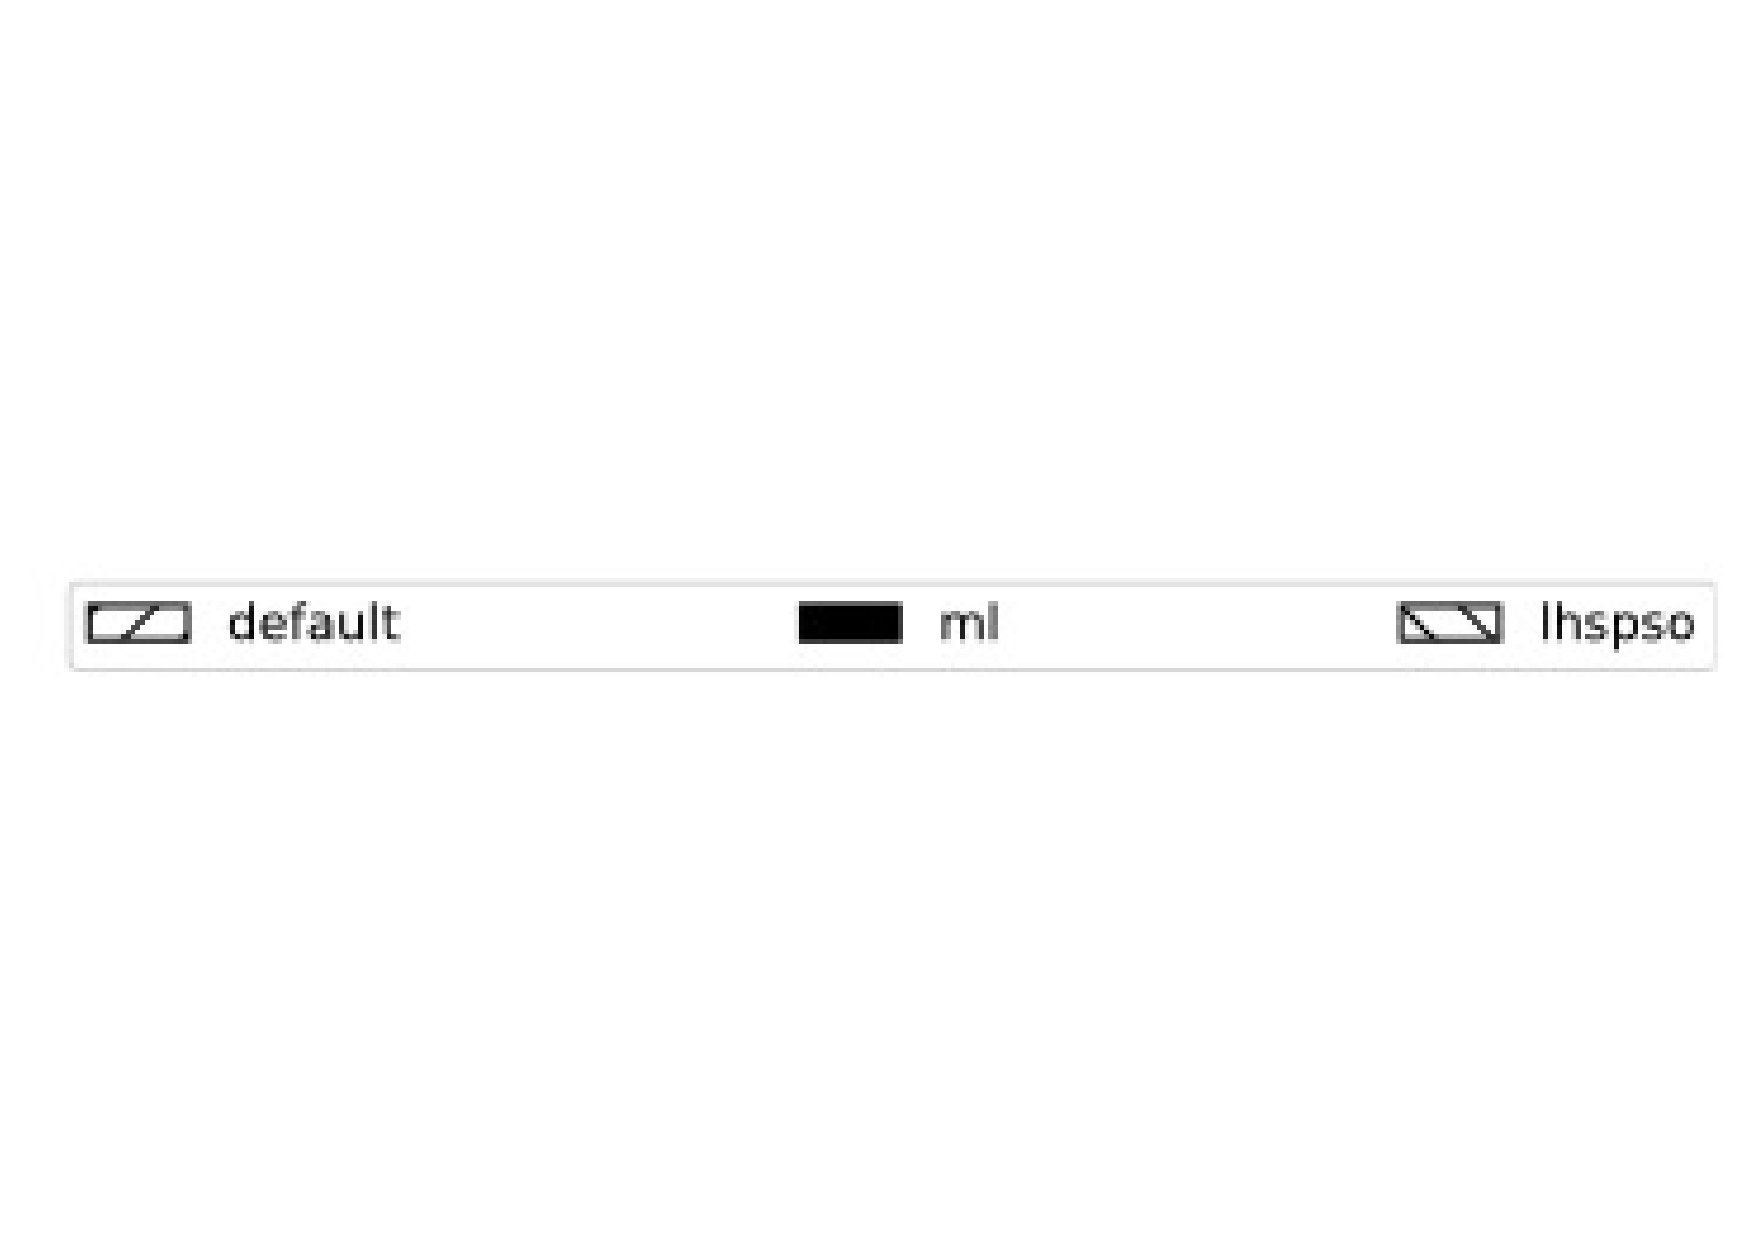
\includegraphics[width=0.45\textwidth]{figures/t_legend.pdf}
\end{subfigure}

\begin{subfigure}{0.5\textwidth}
	\centering
	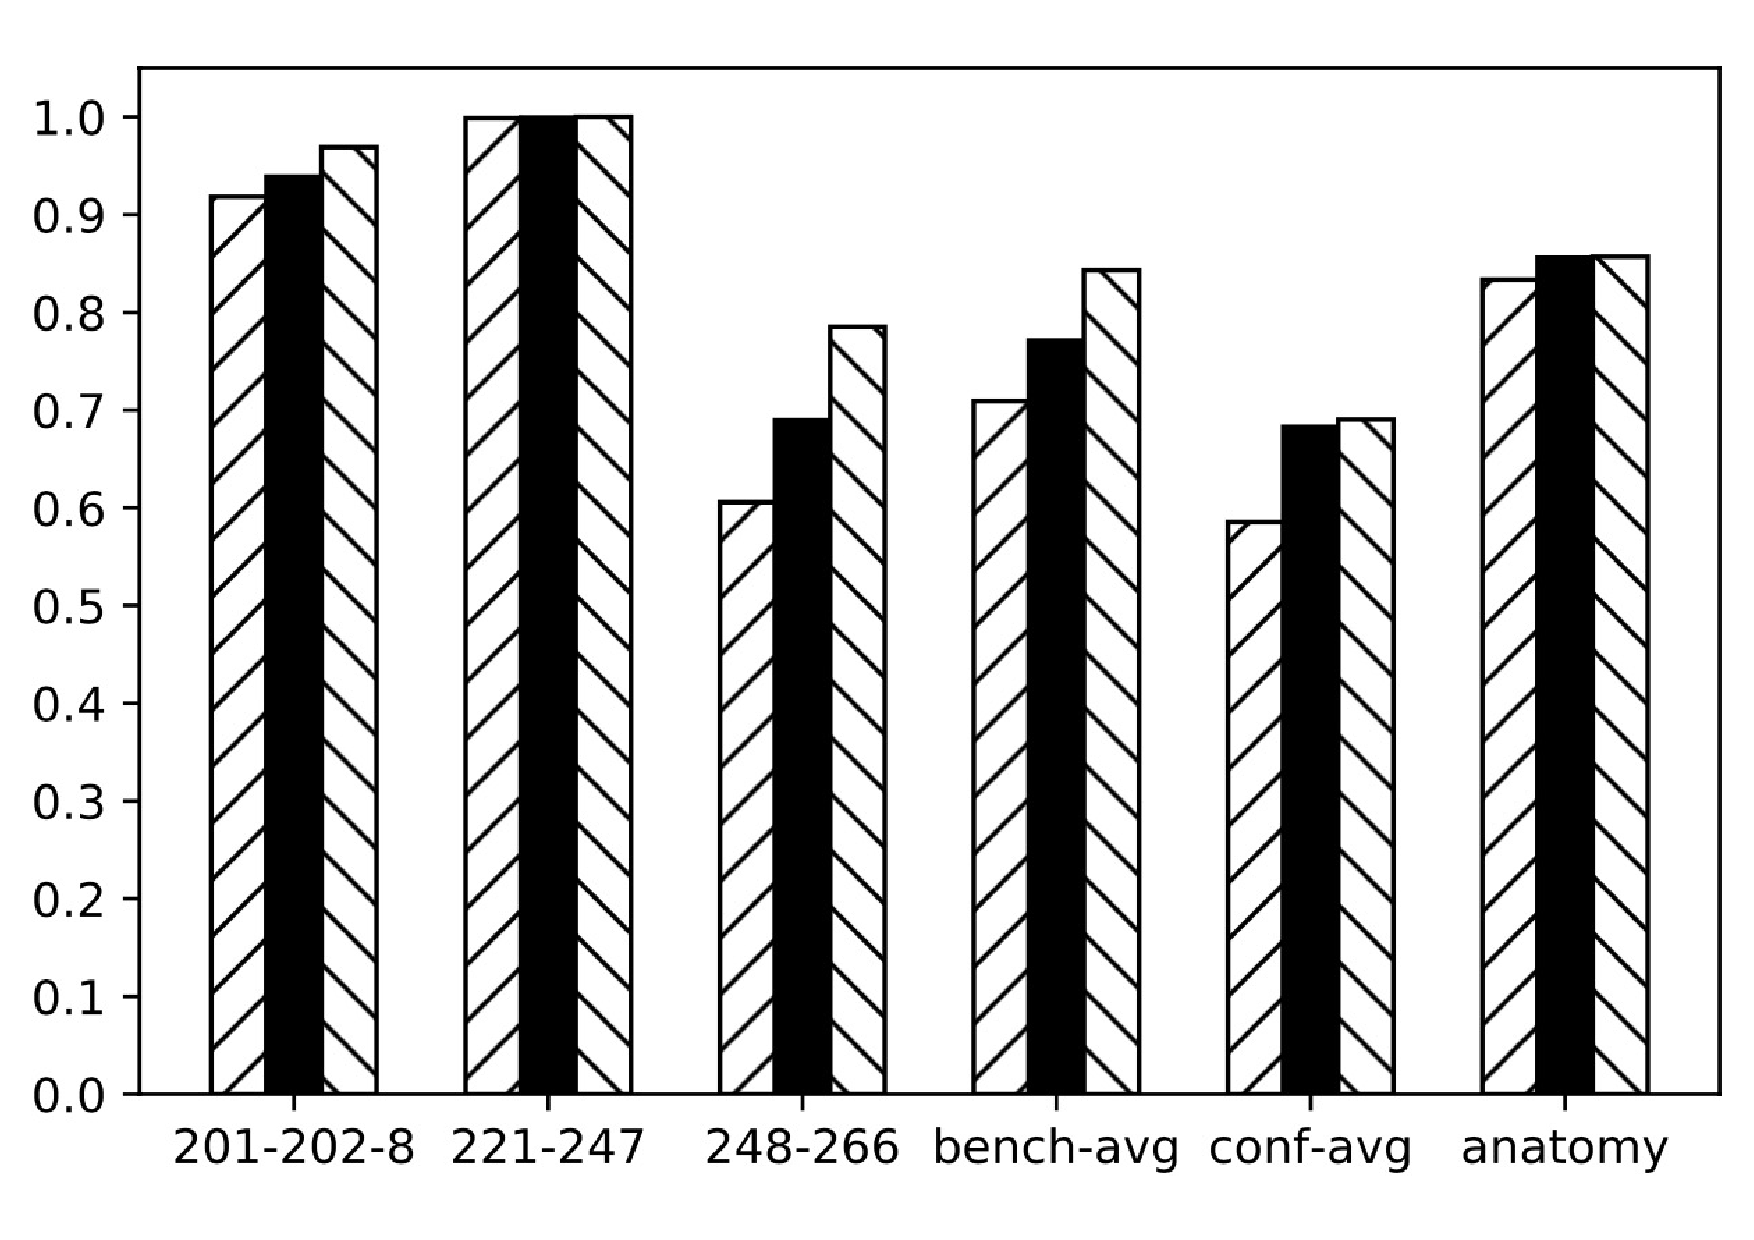
\includegraphics[width=\textwidth]{data_figs/MulRegress_Falcon_AO_F1.pdf}
\end{subfigure}
\caption{The F1-Measure of Falcon-AO}
\label{fig:MultiRegress_Falcon-AO_F1-Measure}
\end{figure}

First look at the F1 value experimental results of the Falcon-AO system.
As shown \ref{fig:MultiRegress_Falcon-AO_F1-Measure}, it can be clearly seen that basically on each data set, the system has significantly improved F1 value compared to the default parameter (default tuning method) after the ml tuning method, and this improvement does not exceed the ideal situation The upper limit, which is in line with experimental expectations.
Among them, the conference dataset has the most improvement, about 16.6\% improvement, and it is very close to the tuning result of the lhspso method. This may be because the ontology in this dataset is real and has practical significance, machine learning model can easily find the rules of parameter prediction in such datasets.
At the same time, the overall average F-value of the benchmark is also significantly improved by 6.24\%, which shows that the default parameter configuration does not fully exert the capabilities of the matching system. The lhspso tuning method reflects the room for improvement. Our proposed ml tuning method is constantly approaching this upper limit.
The main improvement of Falcon-AO on the benchmark dataset is still derived from the improvement of the task 248-266. This task has a large change in partial structure. It is not obvious that the ontology in this task is a partial-text layer change, which means that the parameters in the structure matcher of Falcon-AO are more sensitive than those in the text matcher. And changes in these parameters are more likely to affect the matching result.
the \ref{fig:MulRegress_Falcon_AO_P} reflects the change in P-value precision, and the \ref{fig:MulRegress_Falcon_AO_R} reflects the change in R-value recall. The two indicators of F1 value reflect the overall performance of the matching results.
The change of the R value is basically the same as the change of the F1 value. The P value in the 248-266 and anatomy tasks has decreased compared to the default parameter. This may be because of in the Falcon-AO system, the parameters predicted by the ml tuning method are more inclined to improve the recall rate to find more correct matches, and the change of these parameters sacrifices a certain P-value, but the F1-value is still improved in the final balance. From this we can know that the improvement of F1-value in Falcon-AO system mainly comes from the increase of R value.


\begin{figure}[htb!]\centering
\begin{subfigure}{\textwidth}
	\centering
	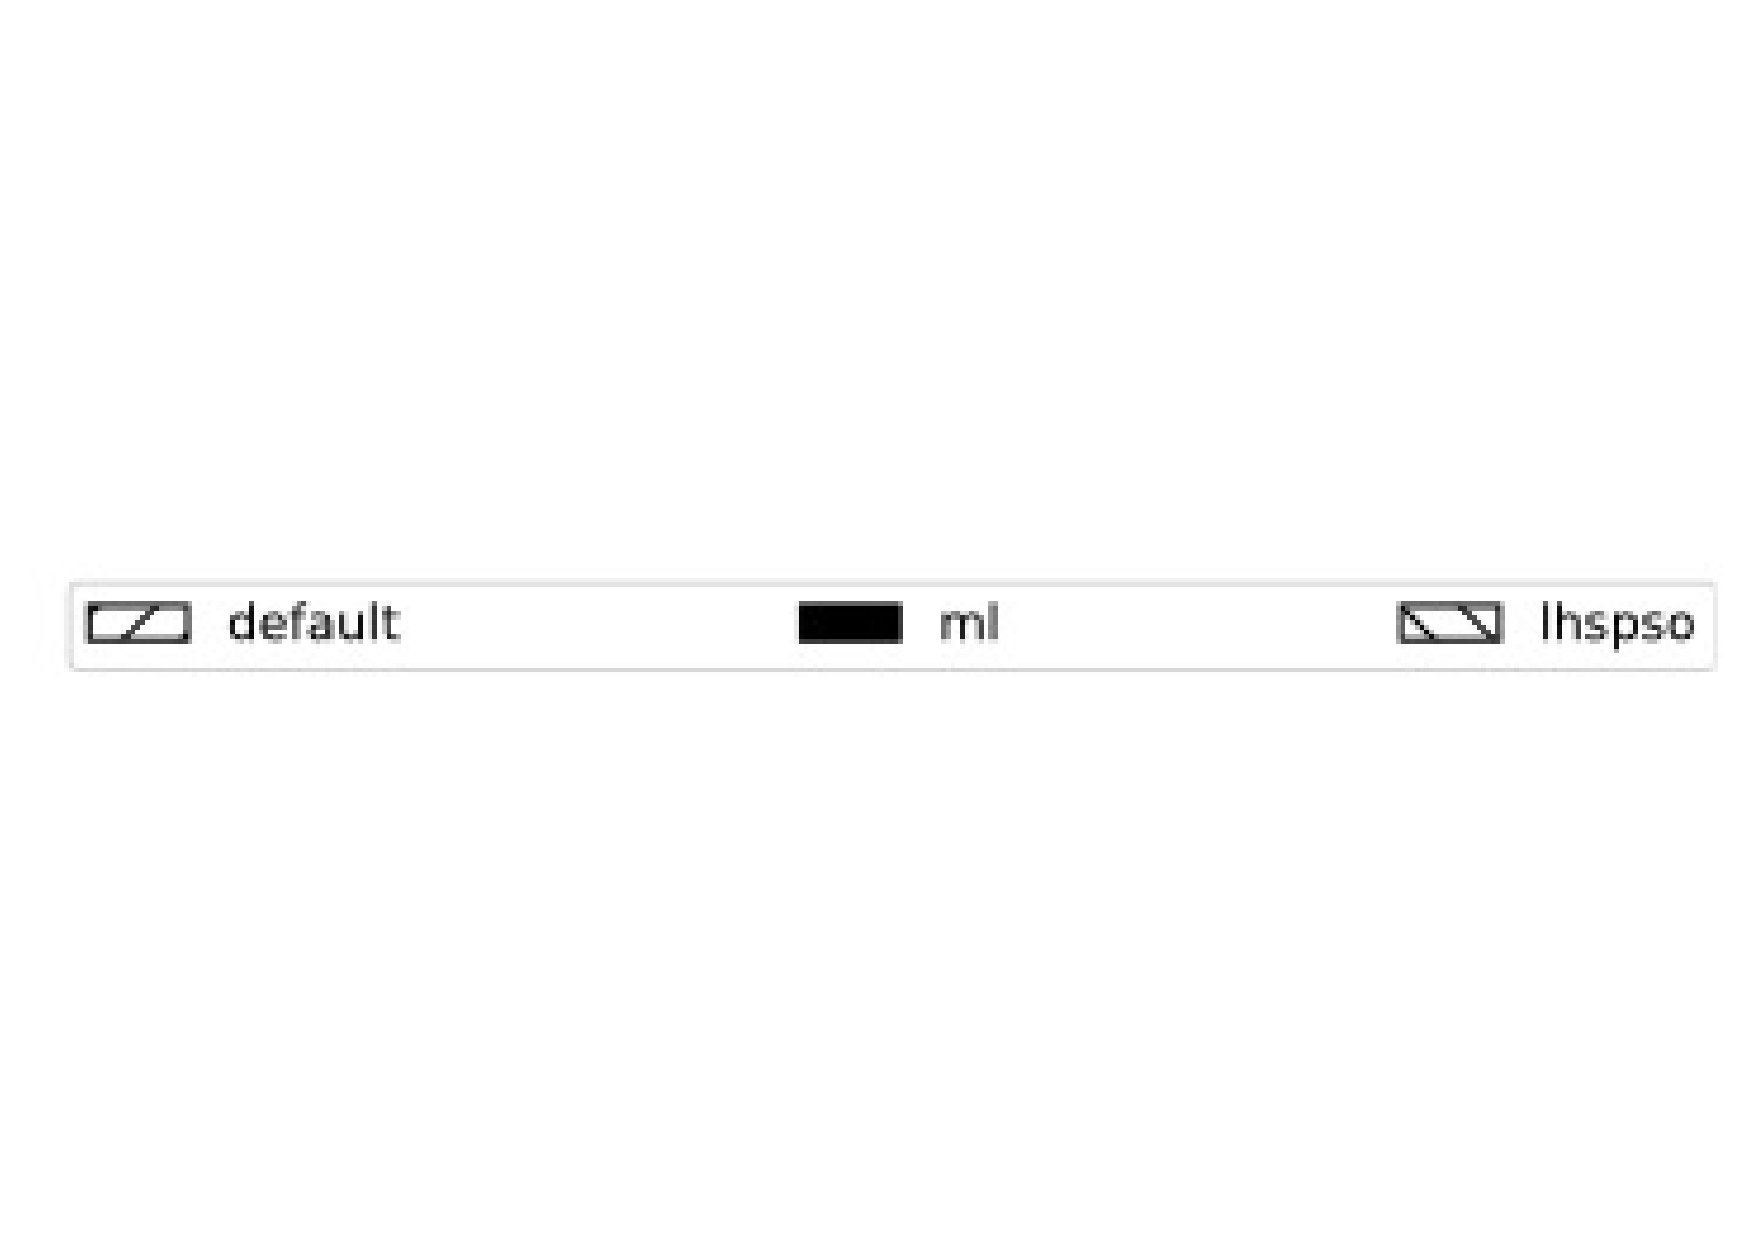
\includegraphics[width=0.45\textwidth]{figures/t_legend.pdf}
\end{subfigure}
\begin{minipage}{0.49\textwidth}
	\centering
	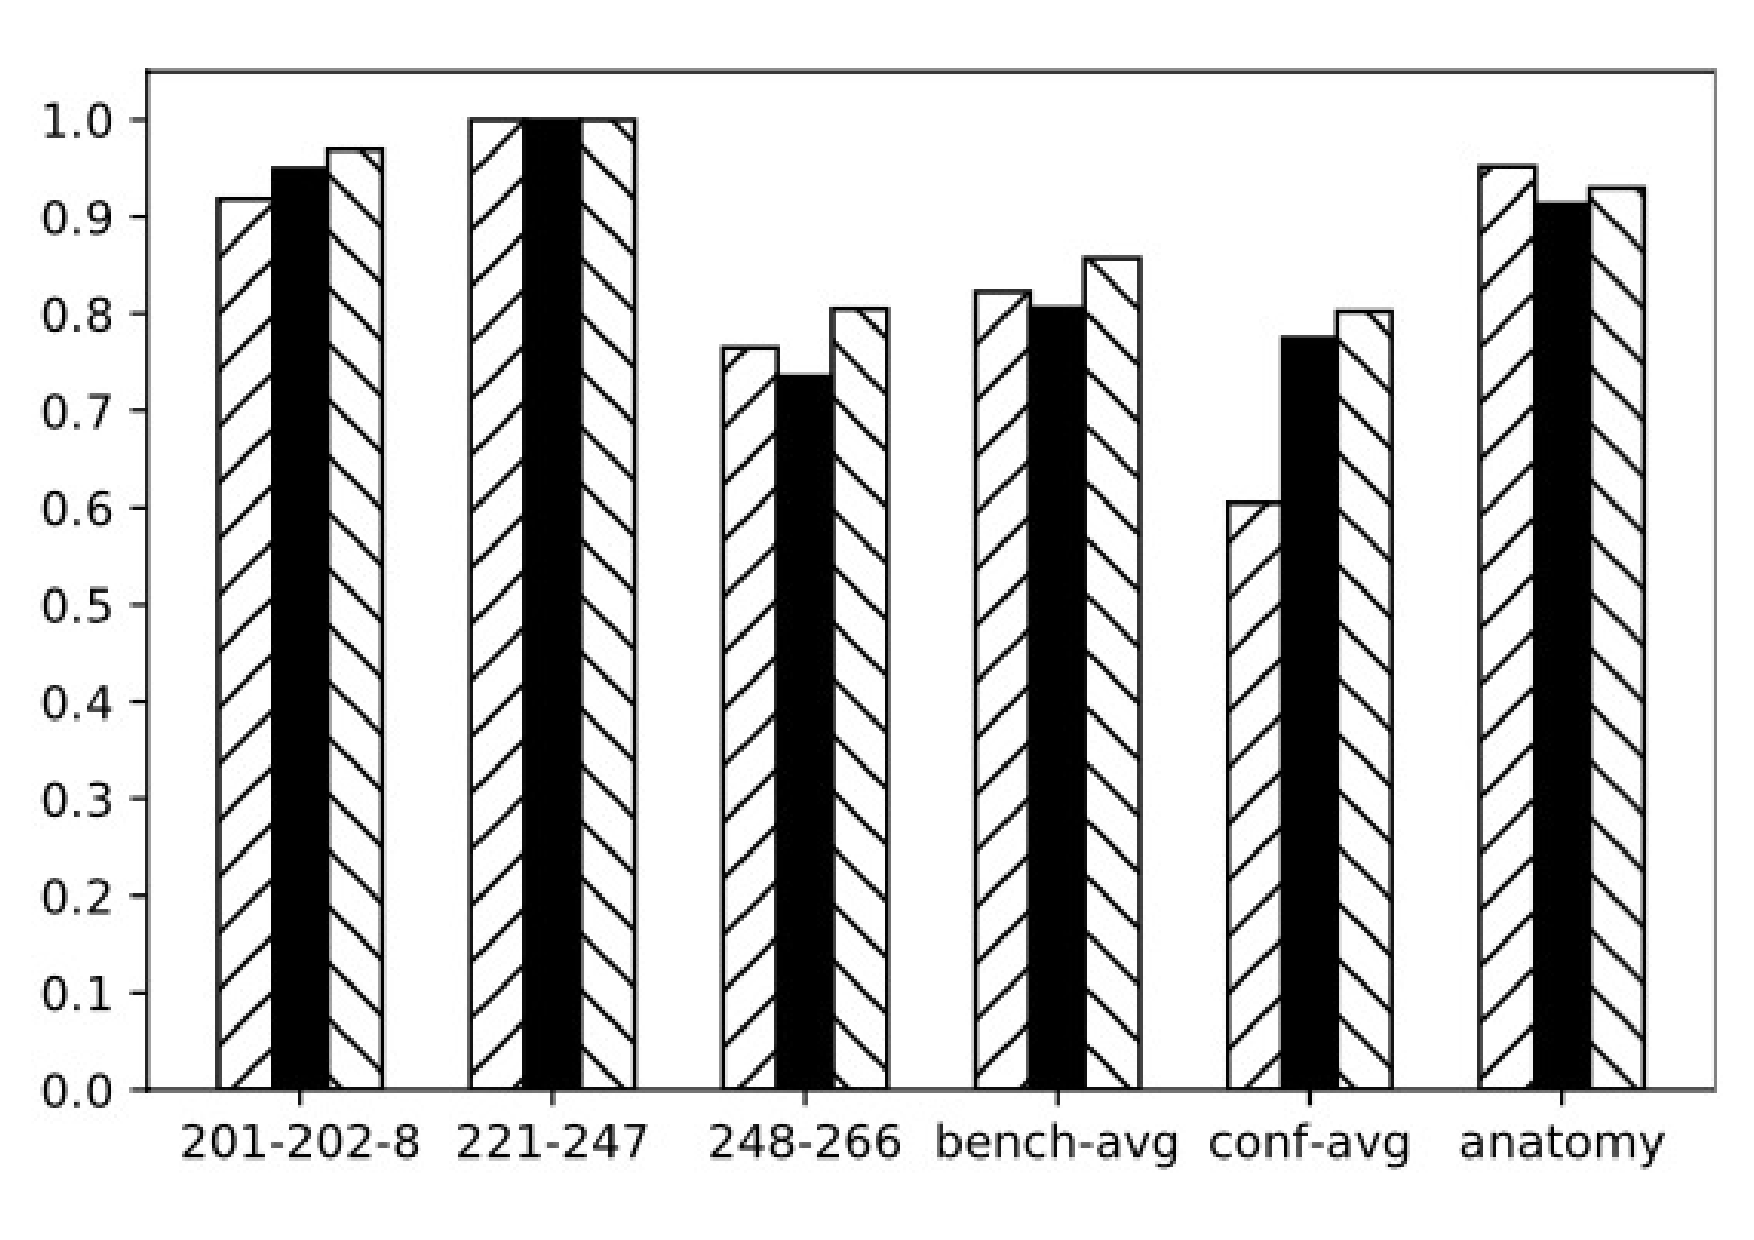
\includegraphics[width=\textwidth]{data_figs/MulRegress_Falcon_AO_P.pdf}
	\captionof{figure}{The P-Measure of Falcon}
	\label{fig:MulRegress_Falcon_AO_P}
\end{minipage}
\begin{minipage}{0.49\textwidth}
	\centering
	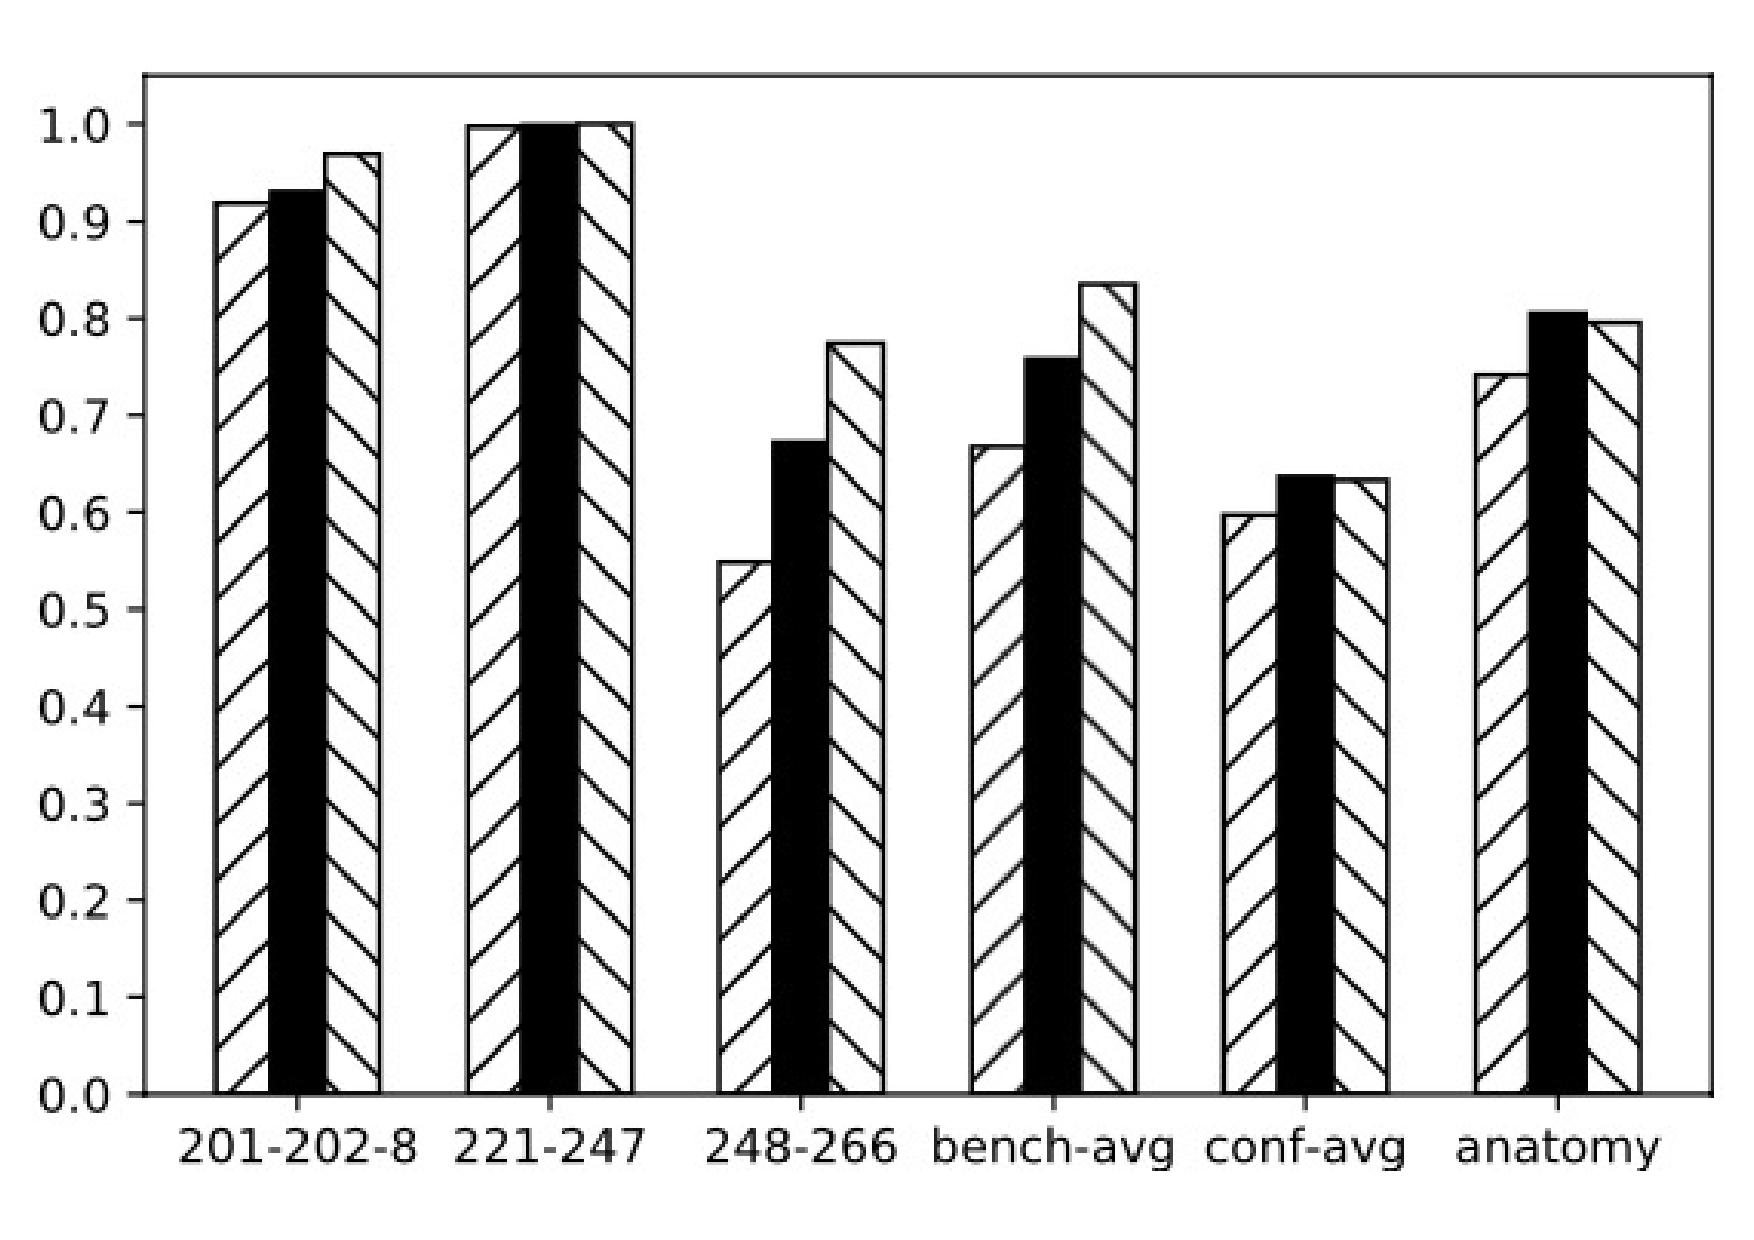
\includegraphics[width=\textwidth]{data_figs/MulRegress_Falcon_AO_R.pdf}
	\captionof{figure}{The R-Measure of Falcon}
	\label{fig:MulRegress_Falcon_AO_R}
\end{minipage}
\end{figure}

The result of the RiMOM is shown in \ref{fig:MultiRegress_RiMOM_F1-Measure}. in general, on each dataset, the system still has a very obvious improvement on F1-value after ml tuning, and the performance on benchmark data set has improved by an average of 13.74\%.
After the parameter tuning of the RiMOM system, the matching accuracy has increased a lot, which almost approaches the upper limit of the ideal situation.
This shows that the model learns very well during the training process, and almost all the laws of parameter changes in the RiMOM system have been learned. So it is very accurate when making predictions, and the result is close to ideal.
At the same time, this also shows that the matching performance of the RiMOM system has a lot of room for improvement, and the study of parameter tuning is of great significance.
In the experimental results of the P and R values shown in \ref{fig:MultiRegress_RiMOM_P} and \ref{fig:MultiRegress_RiMOM_R}, we can find that, unlike Falcon-AO, the accuracy and recall of RiMOM have been improved to different degrees after tuning (the R value increases more greatly) ), which shows that the final improvement of F1-value of the RiMOM mainly comes from the increase of the P and R values.

%\begin{figure}[htb!]\centering
%\begin{subfigure}{\textwidth}
%	\centering
%	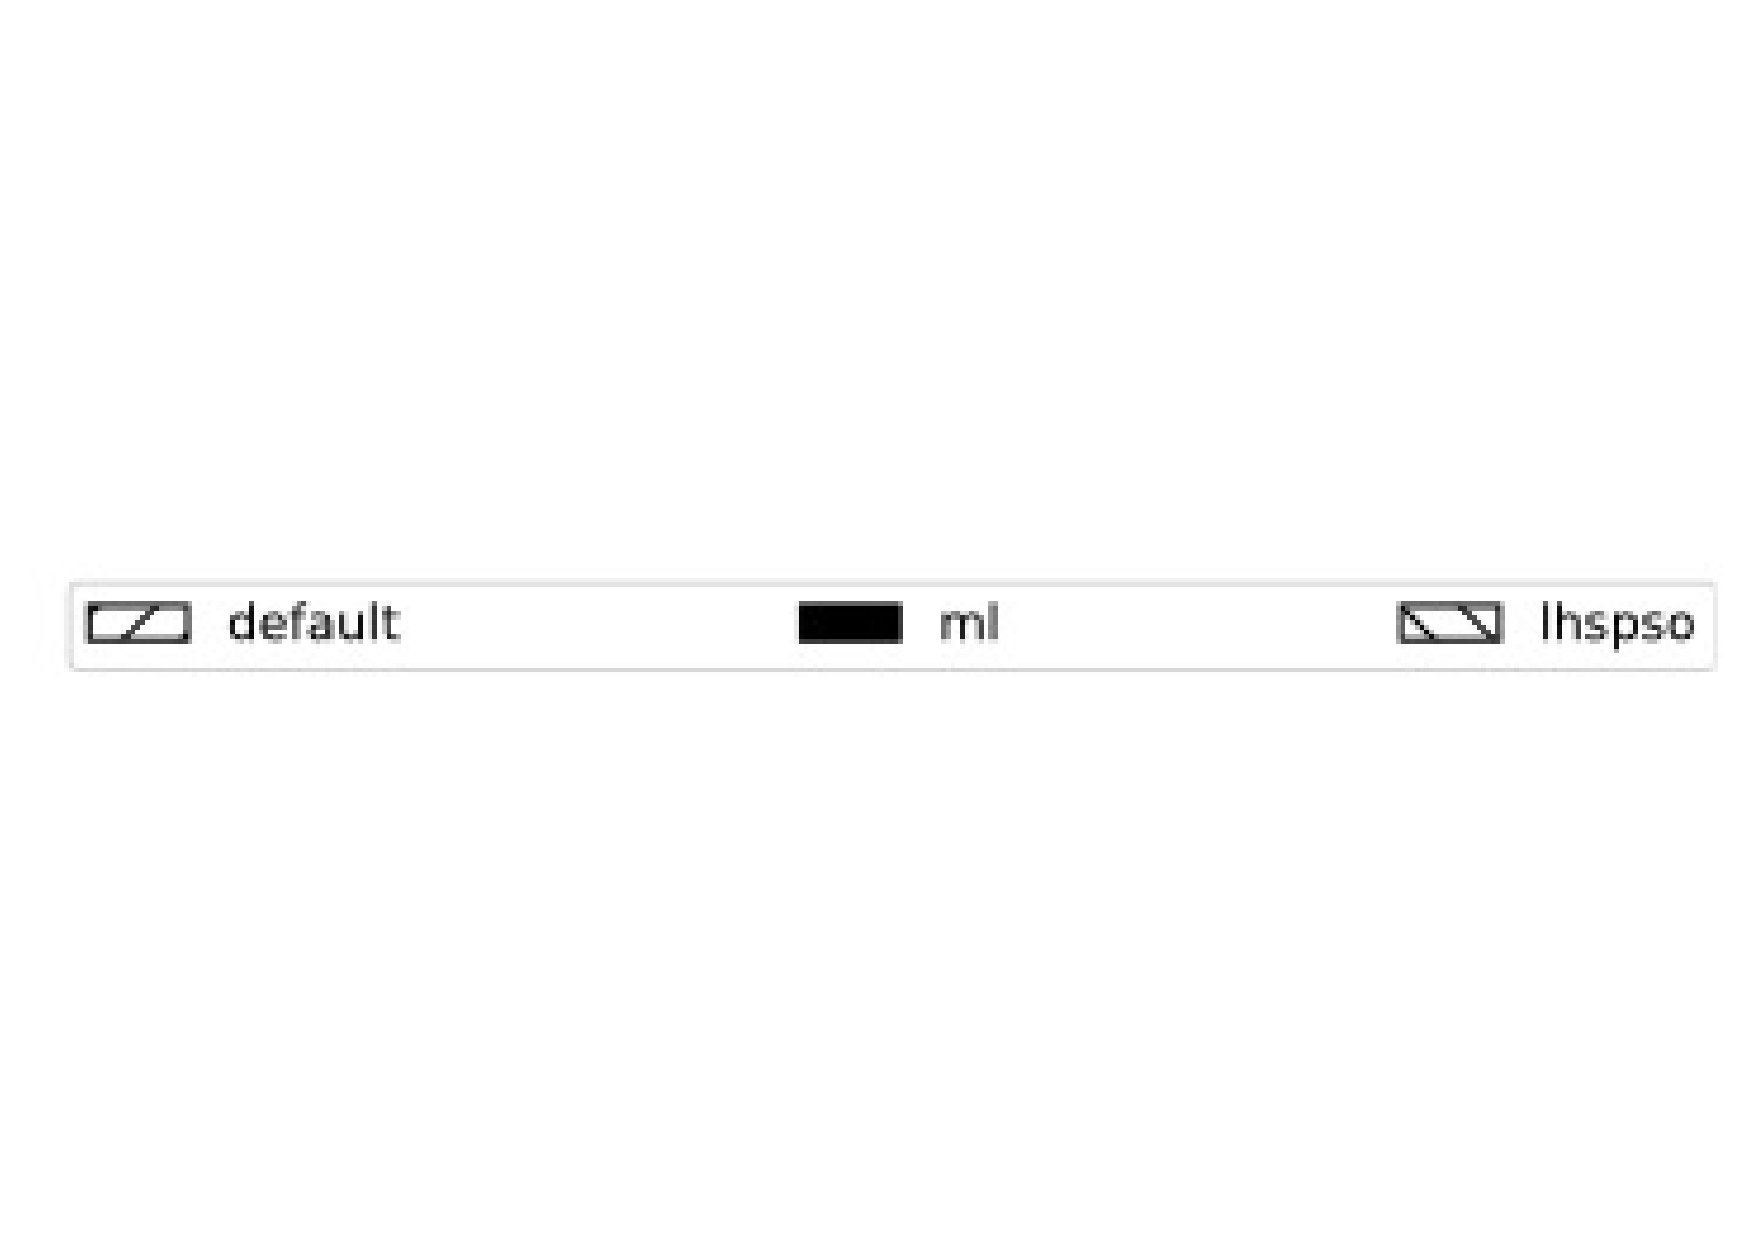
\includegraphics[width=0.45\textwidth]{figures/t_legend.pdf}
%\end{subfigure}
%\begin{minipage}{0.3\textwidth}
%	\centering
%	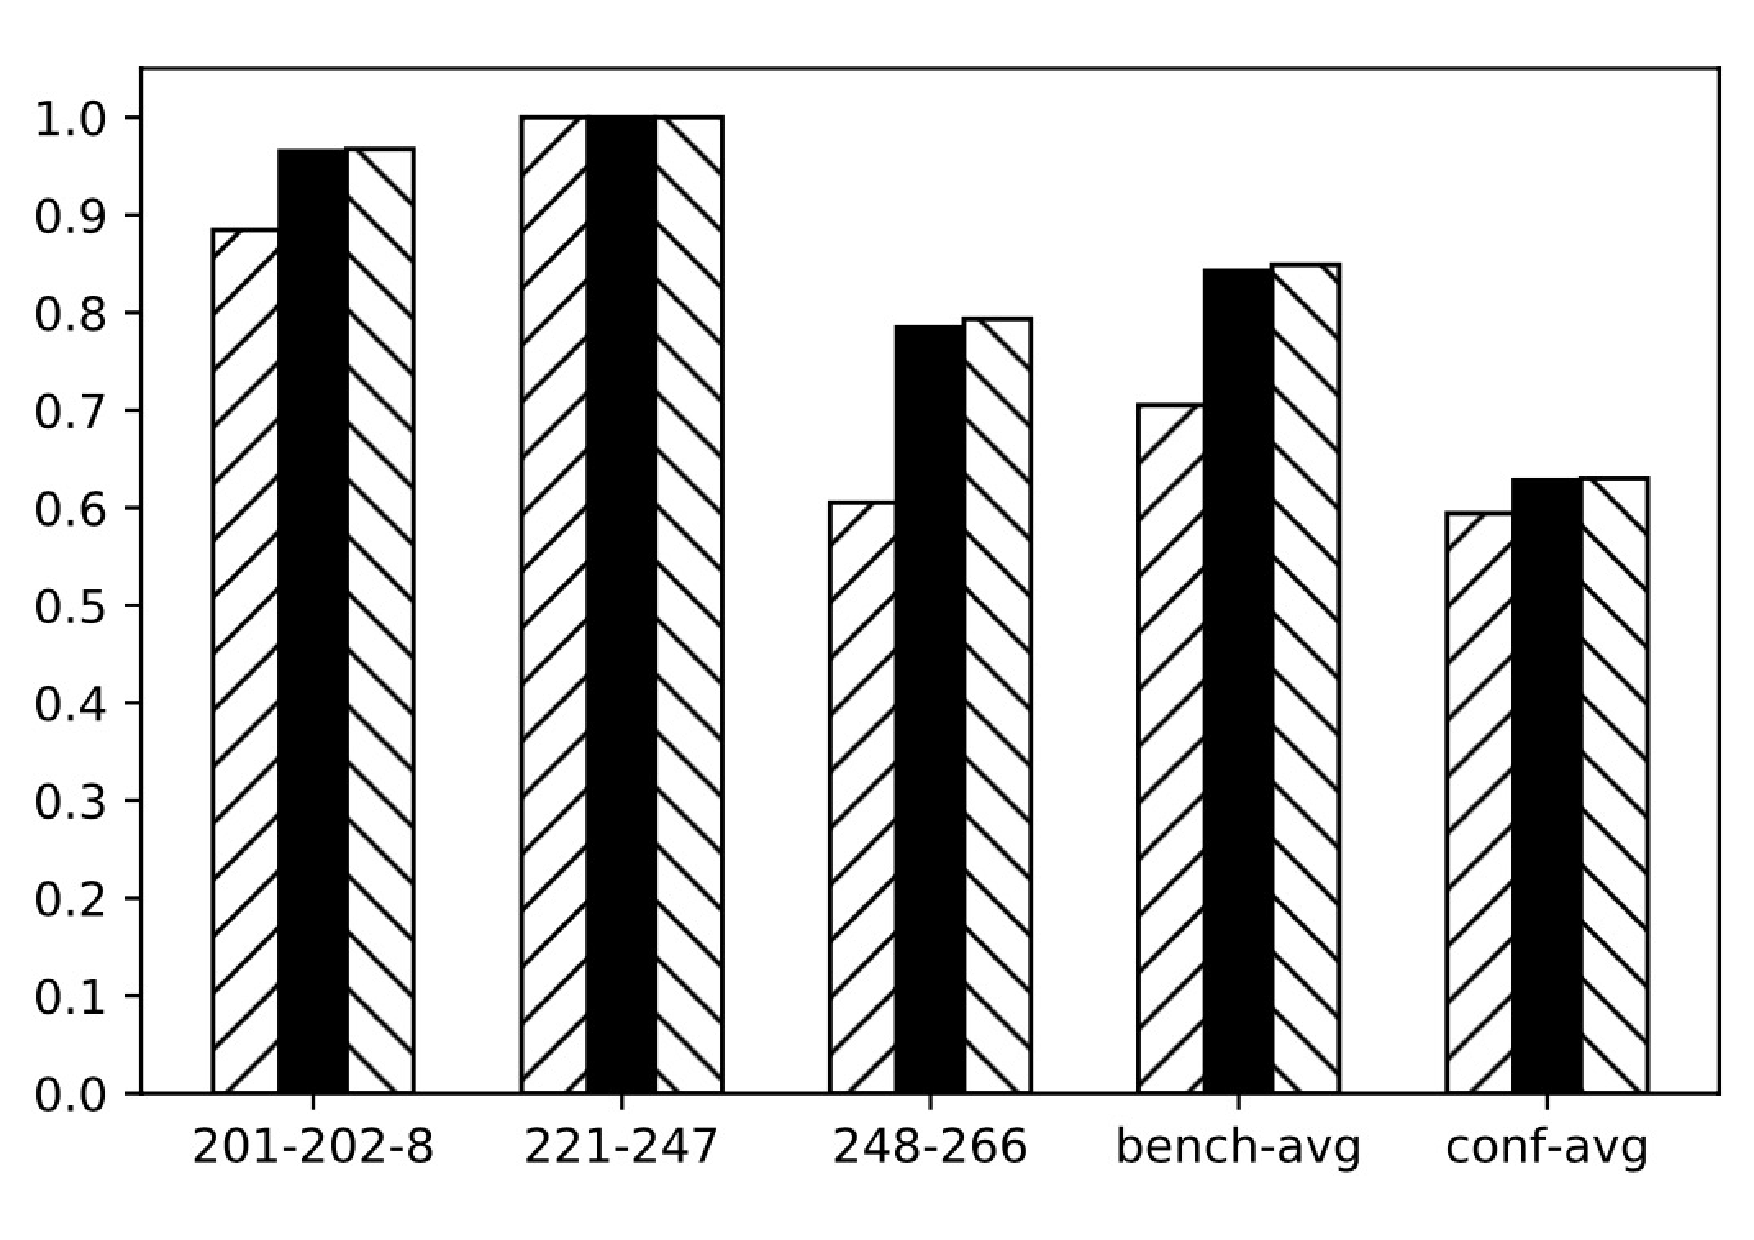
\includegraphics[width=\textwidth]{data_figs/MulRegress_RiMOM_F1.pdf}
%	\captionof{figure}{F1-Measure}
%	\label{fig:MulRegress_RiMOM_F1}
%\end{minipage}
%\begin{minipage}{0.3\textwidth}
%	\centering
%	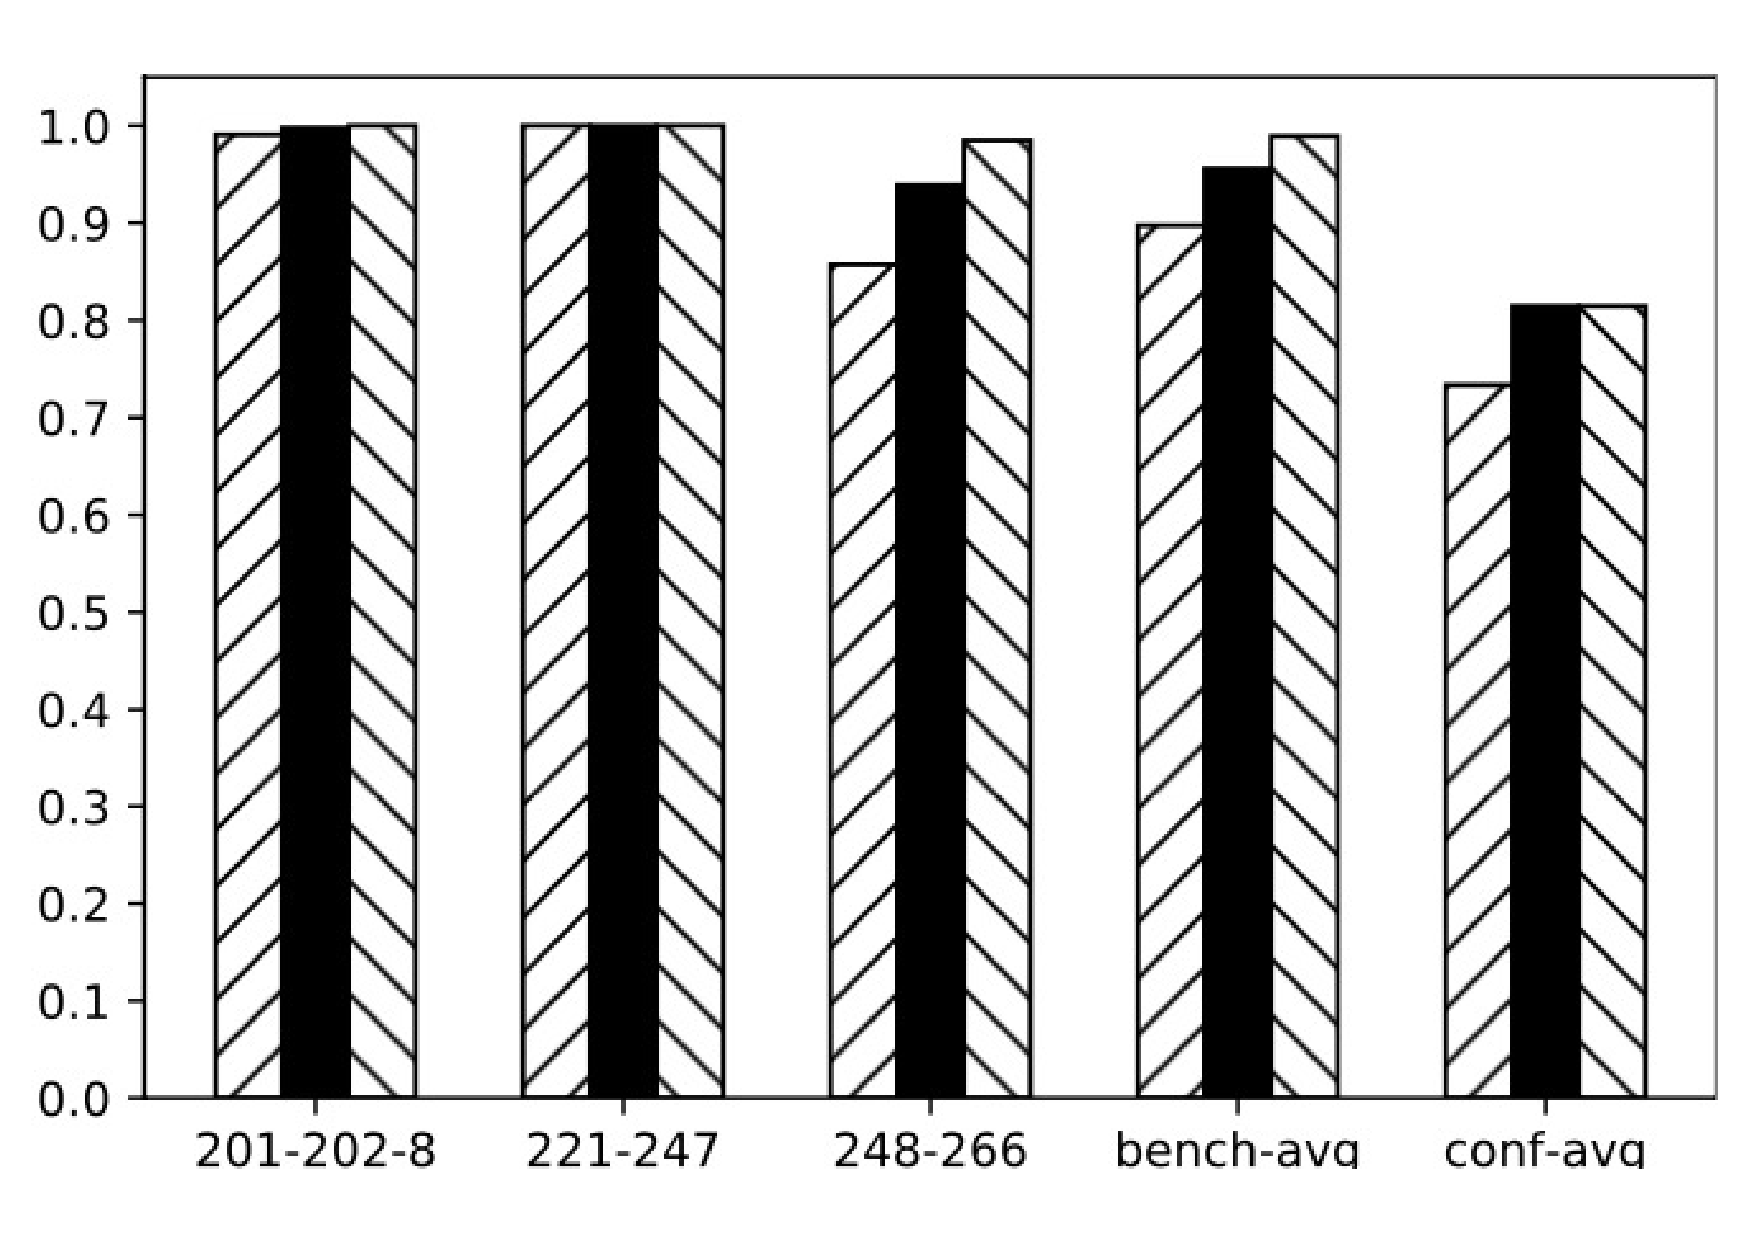
\includegraphics[width=\textwidth]{data_figs/MulRegress_RiMOM_P.pdf}
%	\captionof{figure}{The P-Measure of RiMOM}
%	\label{fig:MulRegress_RiMOM_P}
%\end{minipage}
%\begin{minipage}{0.3\textwidth}
%	\centering
%	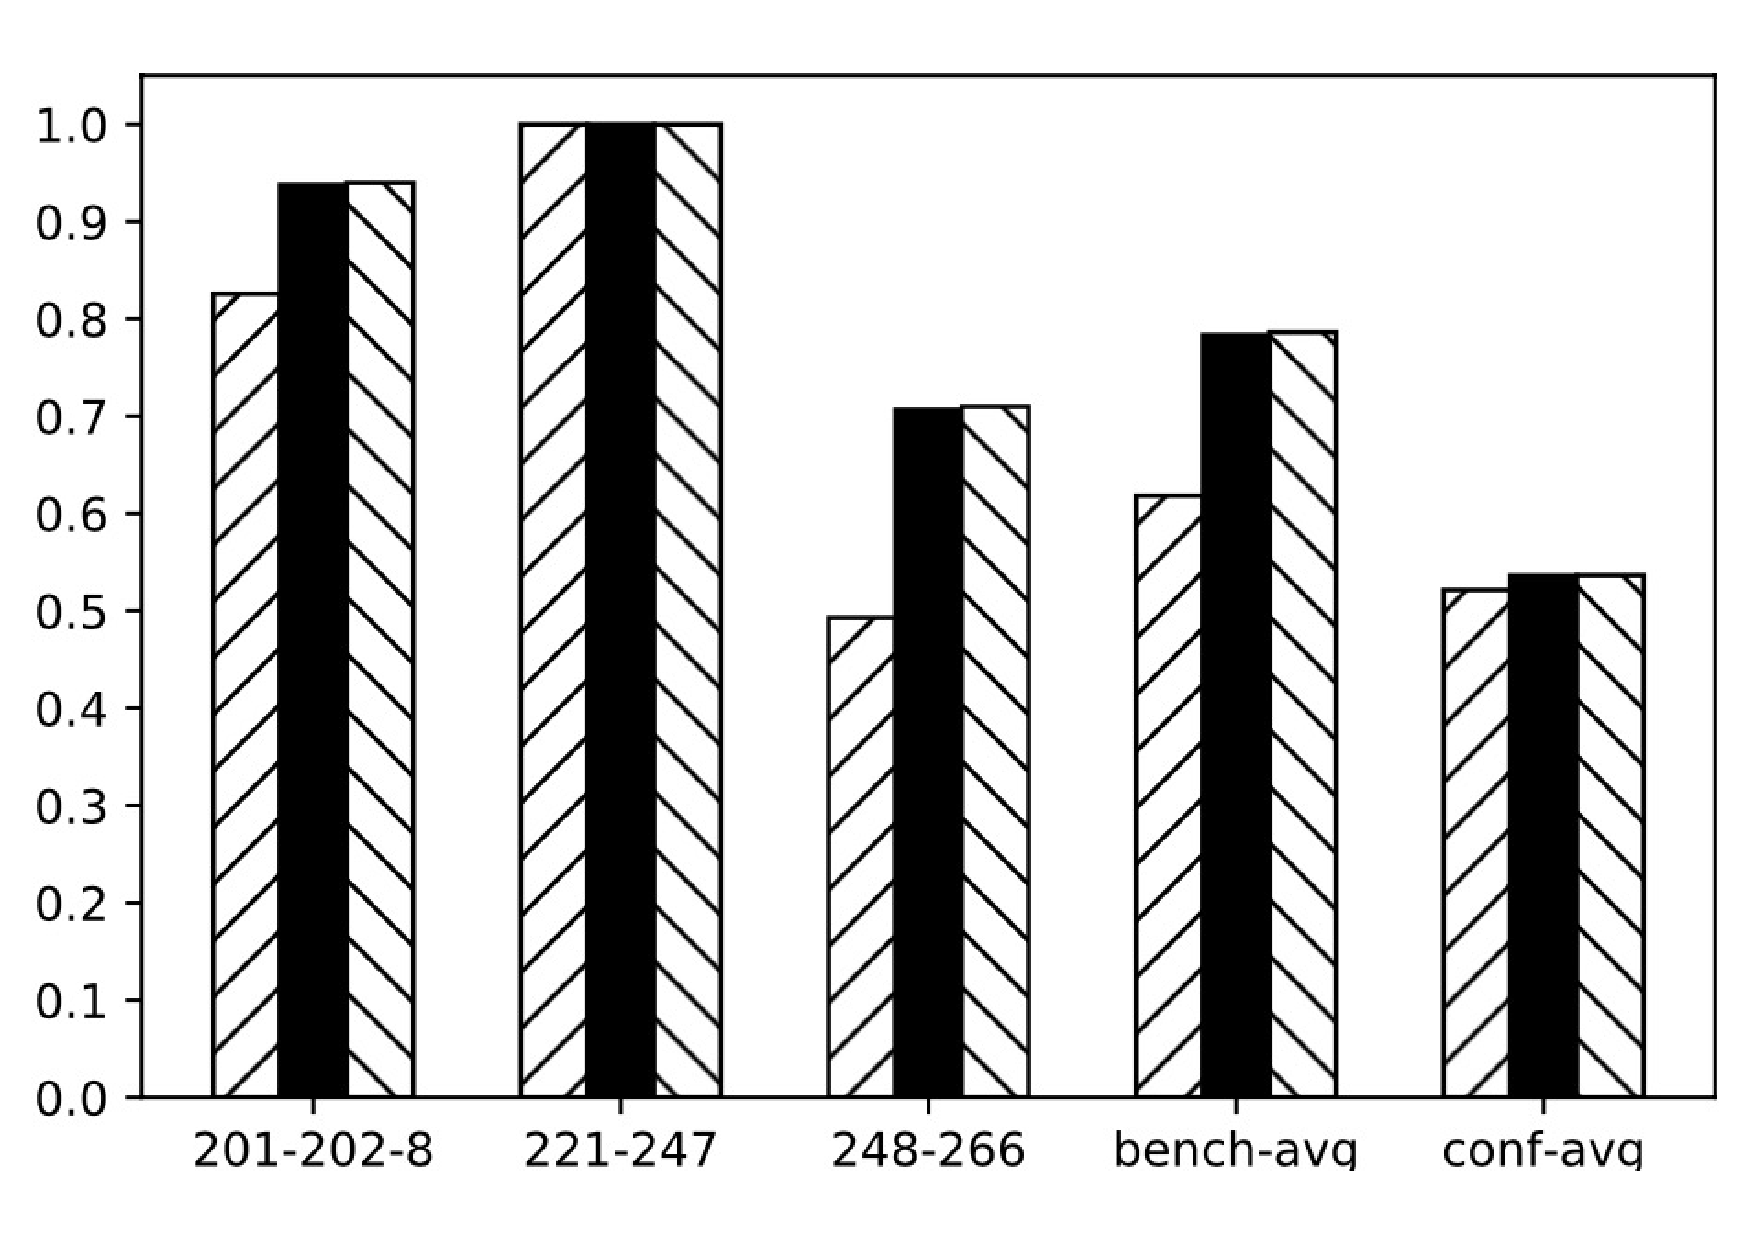
\includegraphics[width=\textwidth]{data_figs/MulRegress_RiMOM_R.pdf}
%	\captionof{figure}{The P-Measure of RiMOM}
%	\label{fig:MulRegress_RiMOM_R}
%\end{minipage}
%\end{figure}

\begin{figure}[htb!]\centering
\begin{subfigure}{\textwidth}
	\centering

\includegraphics[width=0.45\textwidth]{figures/t_legend.jpg}
\end{subfigure}
\begin{subfigure}{0.3\textwidth}
	\centering
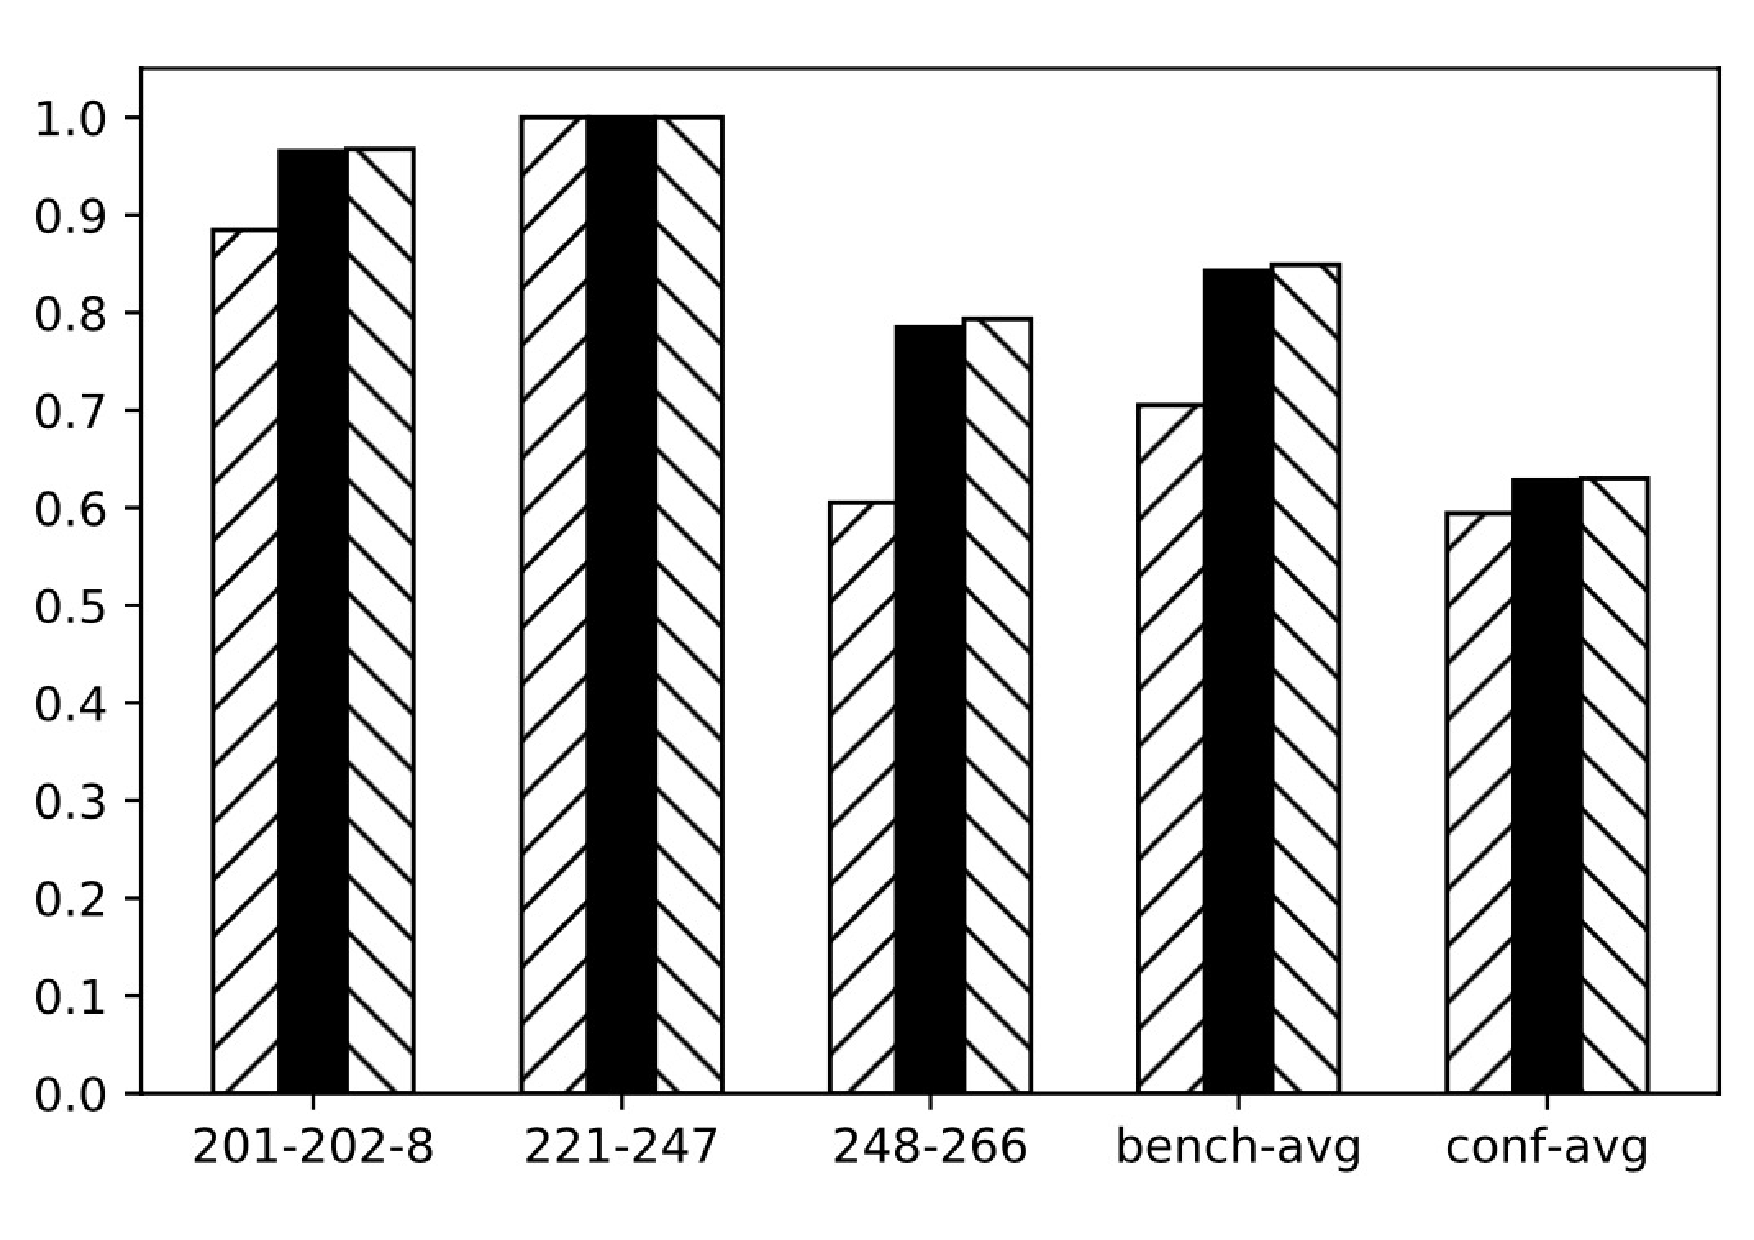
\includegraphics[width=\textwidth]{data_figs/MulRegress_RiMOM_F1.pdf}
\caption{F1-Measure}
\label{fig:MultiRegress_RiMOM_F1-Measure}
\end{subfigure}
%\vskip 1em
\begin{subfigure}{0.3\textwidth}
	\centering
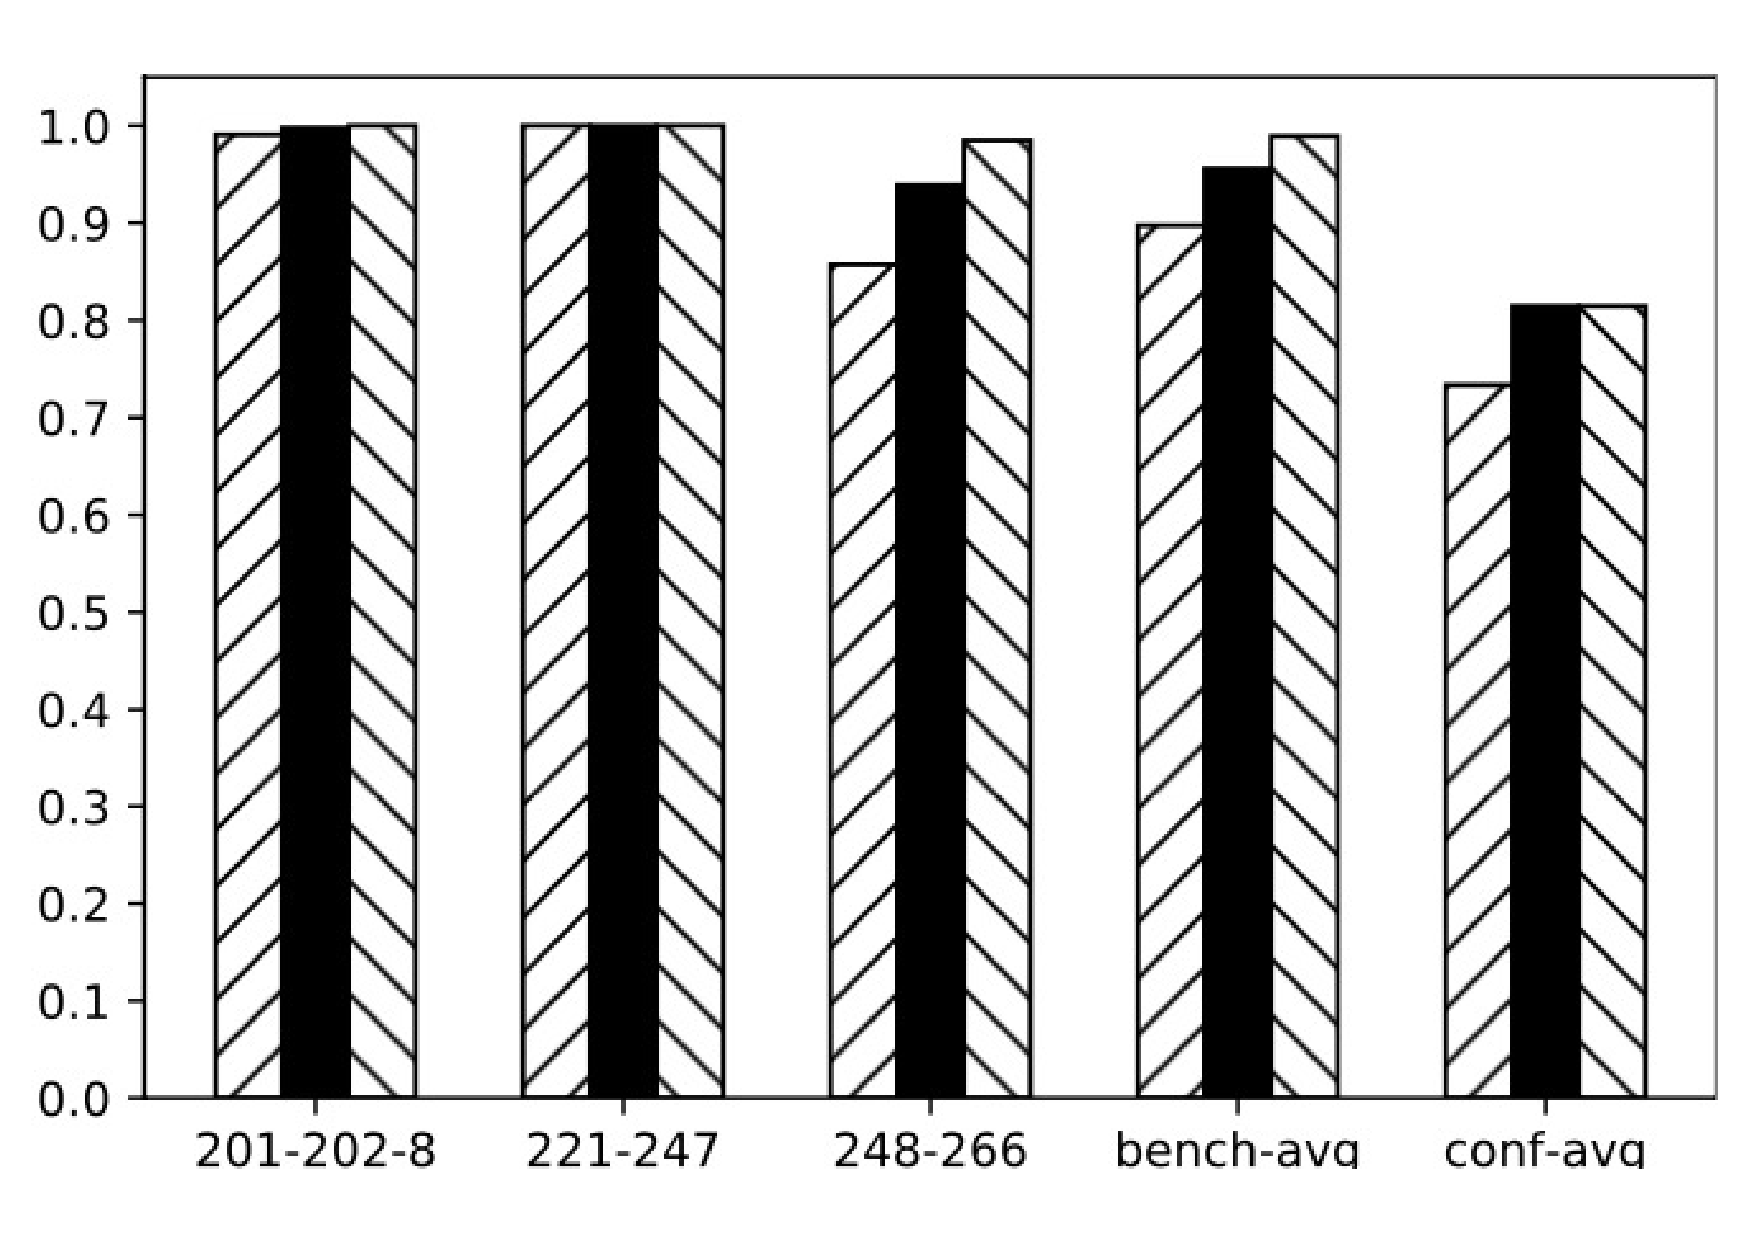
\includegraphics[width=\textwidth]{data_figs/MulRegress_RiMOM_P.pdf}
\caption{Precision}
\label{fig:MultiRegress_RiMOM_P}
\end{subfigure}
\begin{subfigure}{0.3\textwidth}
	\centering
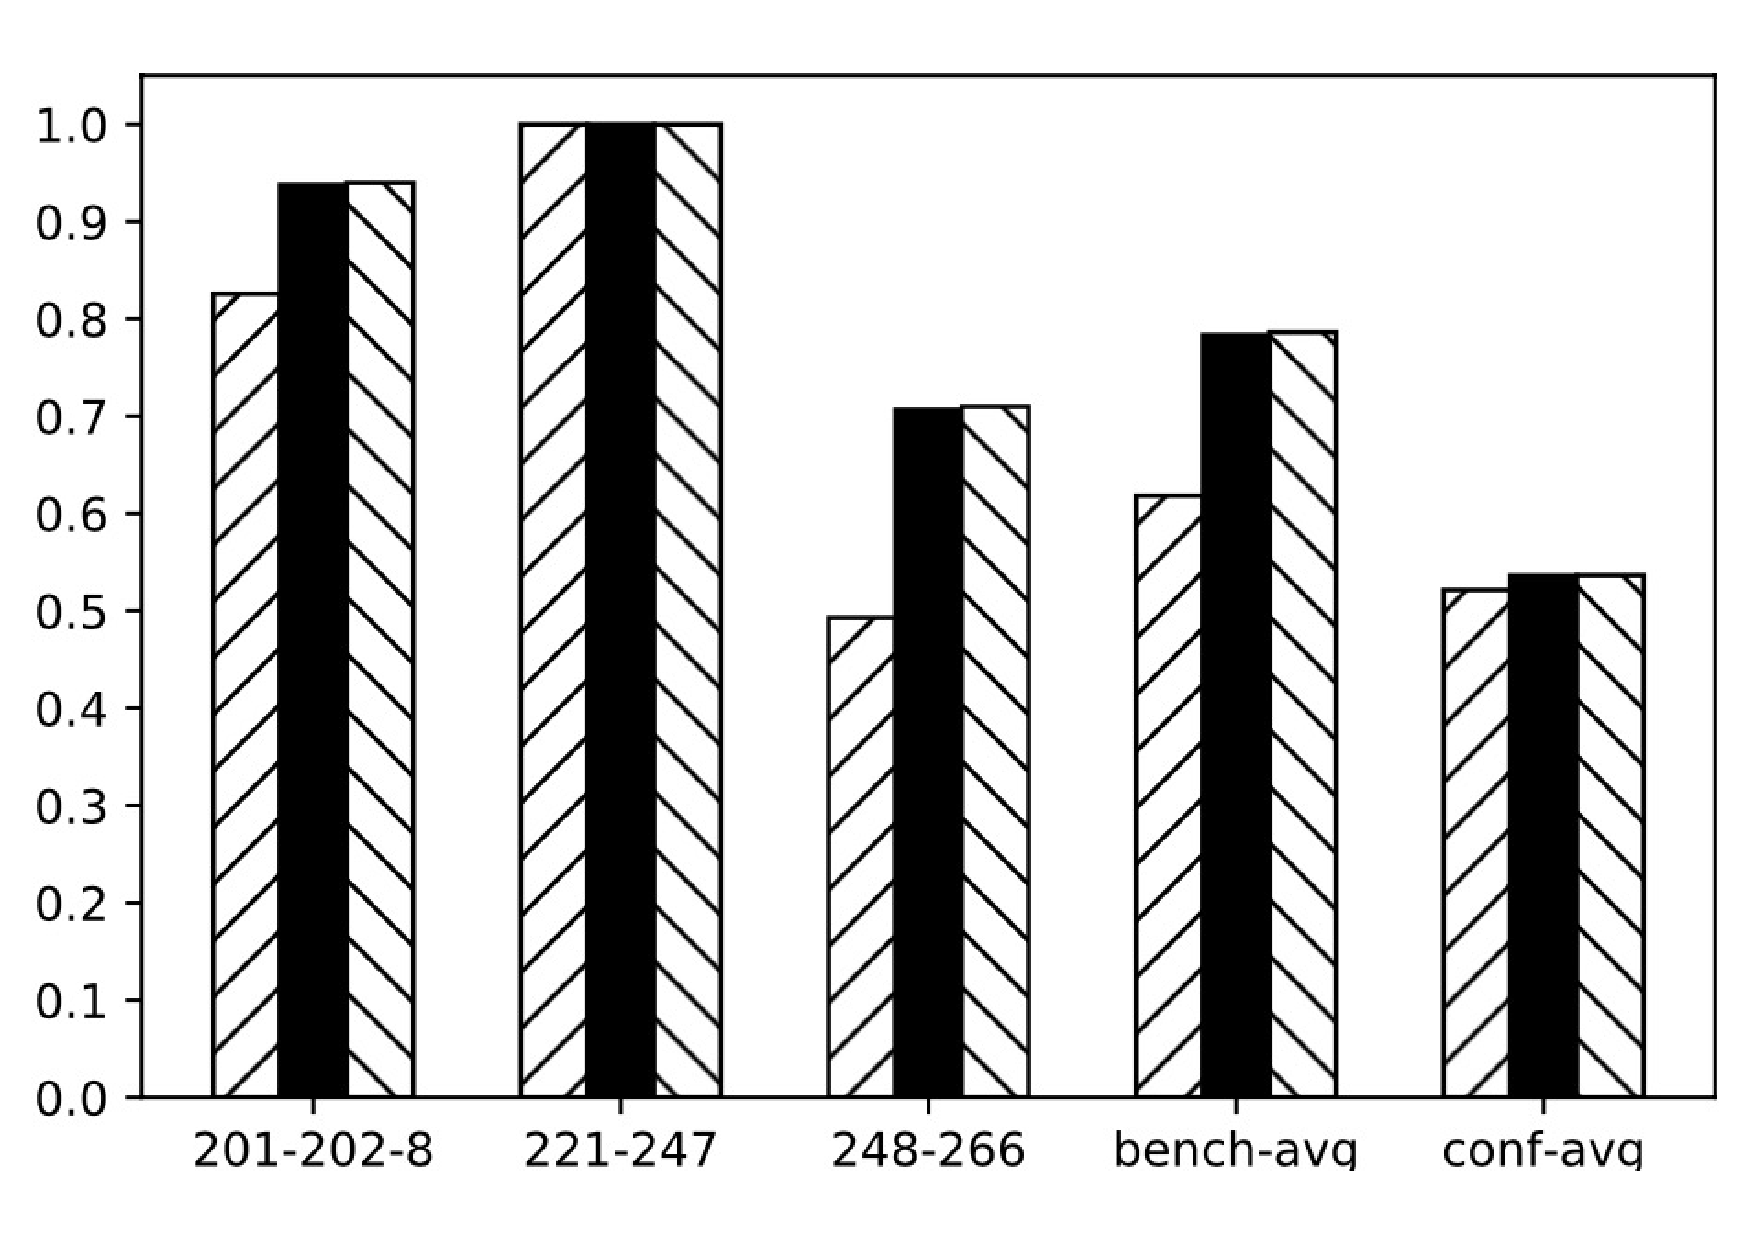
\includegraphics[width=\textwidth]{data_figs/MulRegress_RiMOM_R.pdf}
\caption{Recall}
\label{fig:MultiRegress_RiMOM_R}
\end{subfigure}
\caption{results of RiMOM}
\end{figure}

The \ref{fig:MultiRegress_Lily_F1} shows the experimental results of the F1 value of the Lily system.
Comparing the two systems analyzed before, we can see that Lily's matching performance is not significantly improved after the ml tuning method.
The possible reasons for the analysis are: on the one hand, the Lily system itself has performed very well on some data sets (for example, it maintains a world record of F1 value 0.9 on the benchmark dataset), and its matching algorithm itself is already too complicated to further improve the accuracy by the subsequent parameter tuning.
In other words, the room that Lily can improve through tuning is very small, which can be seen from the upper limit of the lhspso tuning method.
The {\it upper limit} is actually determined by the algorithm of the matching system itself. The tuning is only to approach this upper limit. On the other hand, we found an interesting phenomenon that there is a lot of randomness in the Lily system when running the task script for multiple times, that is, given a certain task, the same set of parameter configuration, running multiple times will have multiple different results.
This {\it randomness} can easily lead to the randomness of the sample labels when constructing the training set, which will cause certain bias to the model training.
Then from \ref{fig:MultiRegress_Lily_P} and \ref{fig:MultiRegress_Lily_R} ,the P-value has an insignificant improvement on some datasets, but the R value has decreased somewhat. These have led to a small increase in the overall F1 value.

\begin{figure}[htb!]\centering
\begin{subfigure}{\textwidth}
	\centering
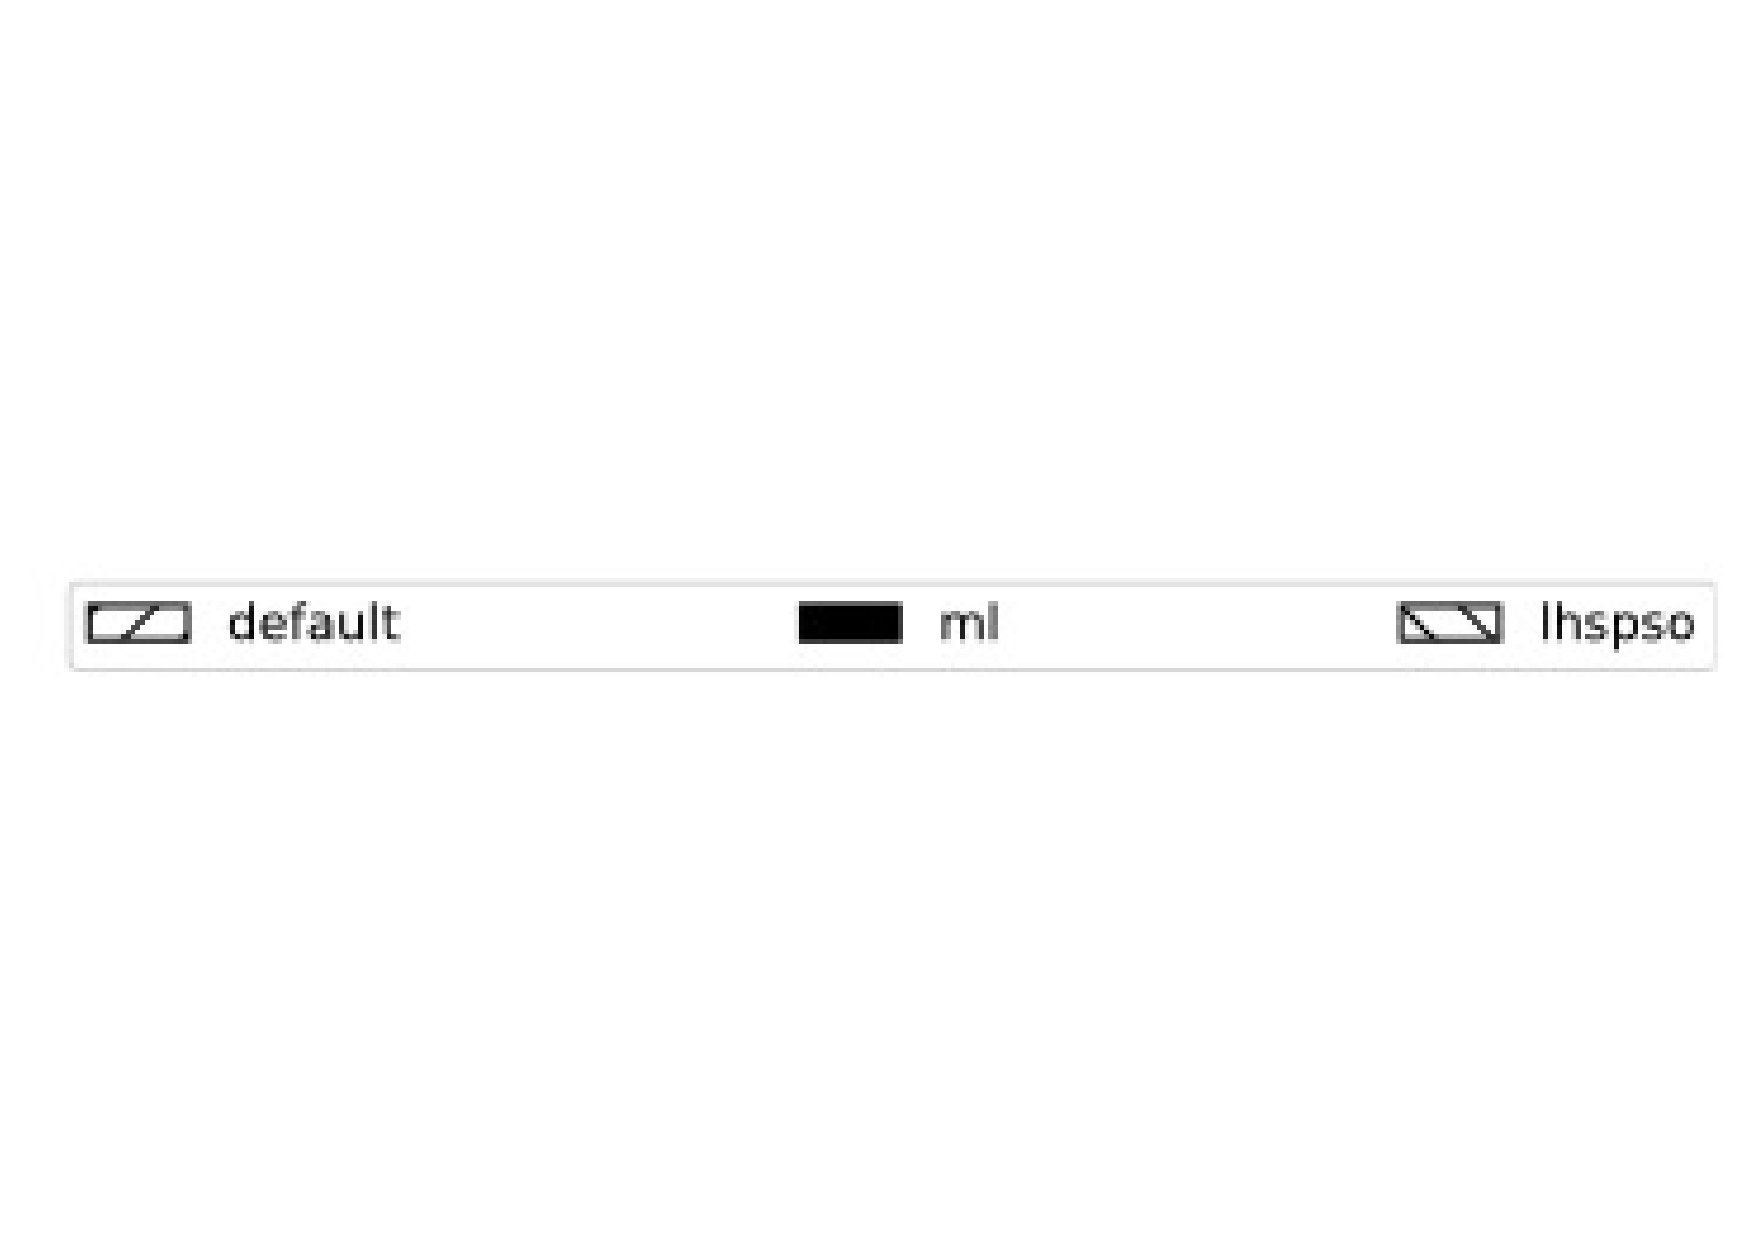
\includegraphics[width=0.45\textwidth]{figures/t_legend.pdf}
\end{subfigure}
\begin{subfigure}{0.3\textwidth}
	\centering
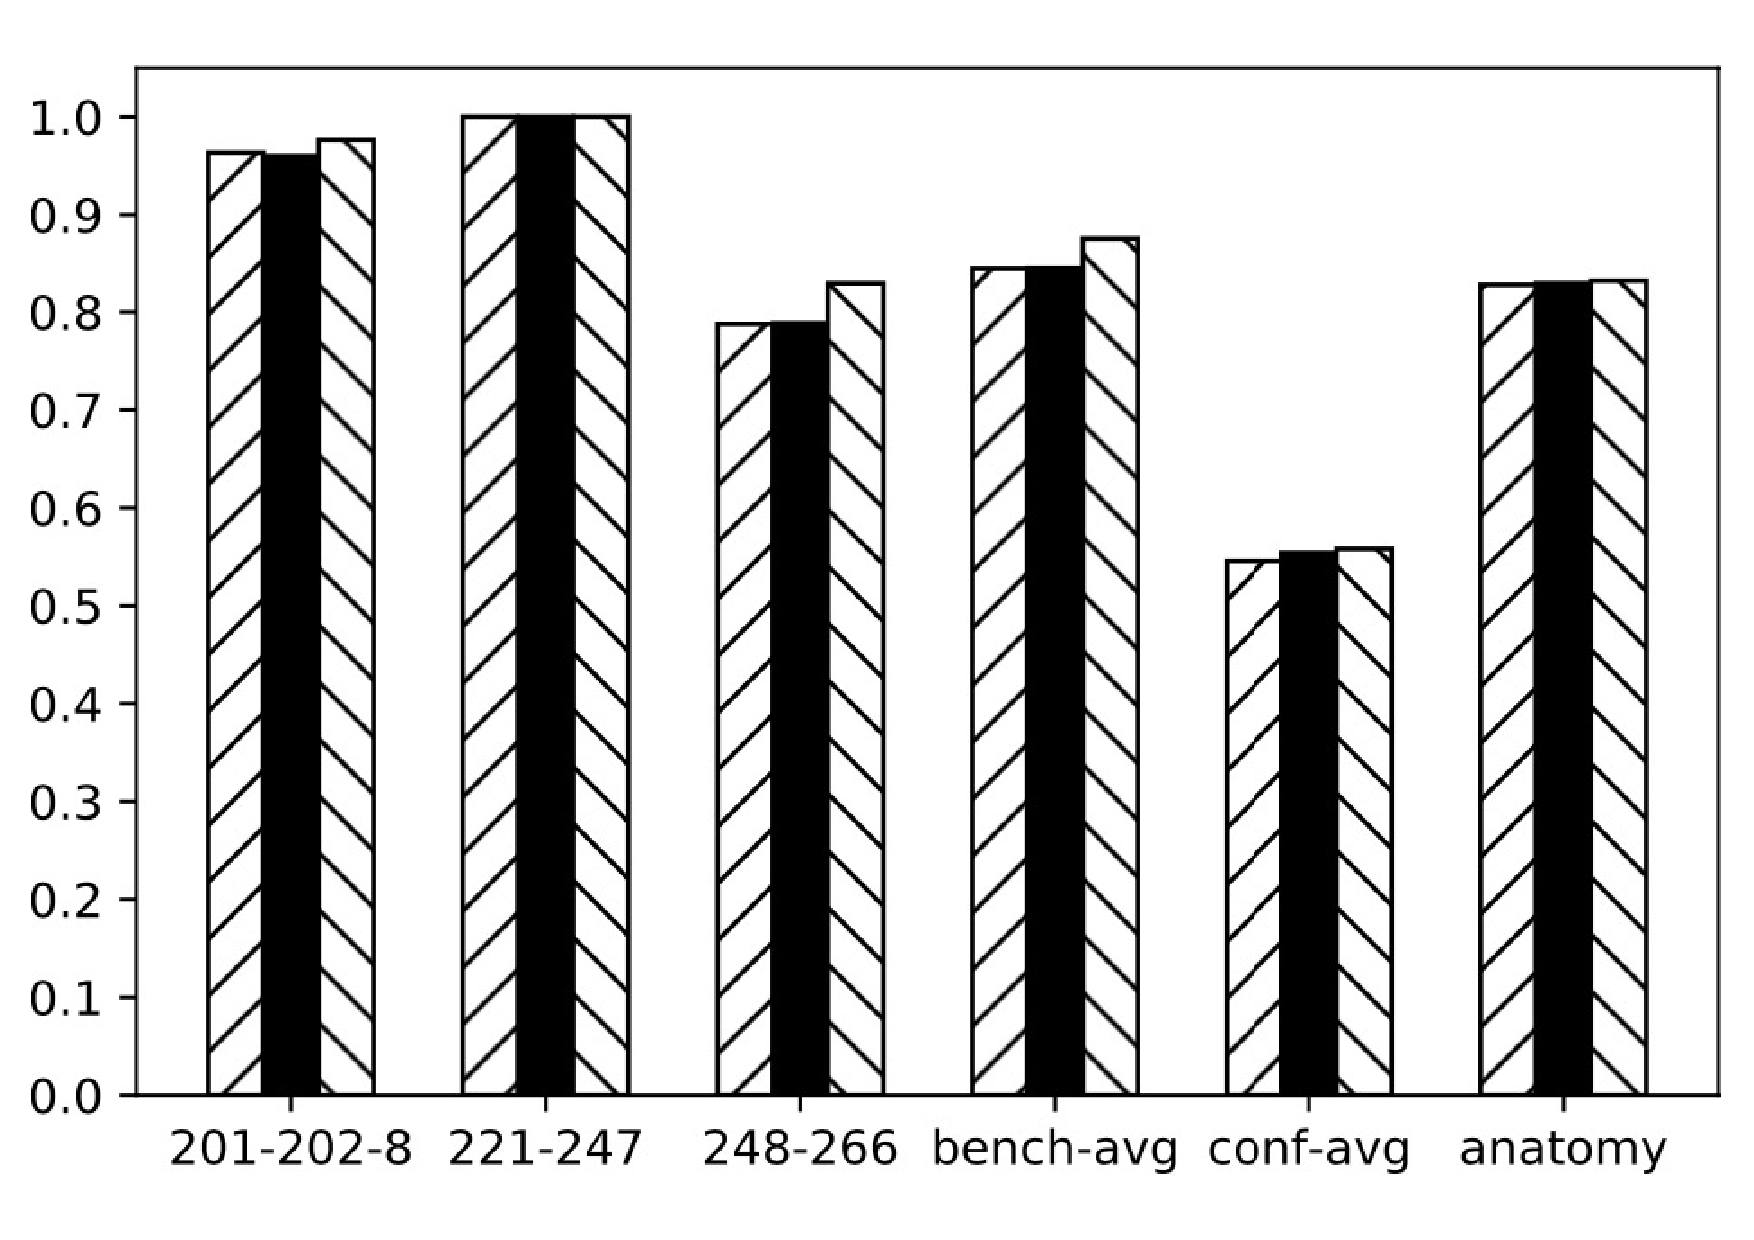
\includegraphics[width=\textwidth]{data_figs/MulRegress_Lily_F1.pdf}
\caption{F1-Measure}
\label{fig:MultiRegress_Lily_F1}
\end{subfigure}
%\vskip 1em
\begin{subfigure}{0.3\textwidth}
	\centering
\includegraphics[width=\textwidth]{data_figs/MulRegress_Lily_P.pdf}
\caption{Precision}
\label{fig:MultiRegress_Lily_P}
\end{subfigure}
\begin{subfigure}{0.3\textwidth}
	\centering
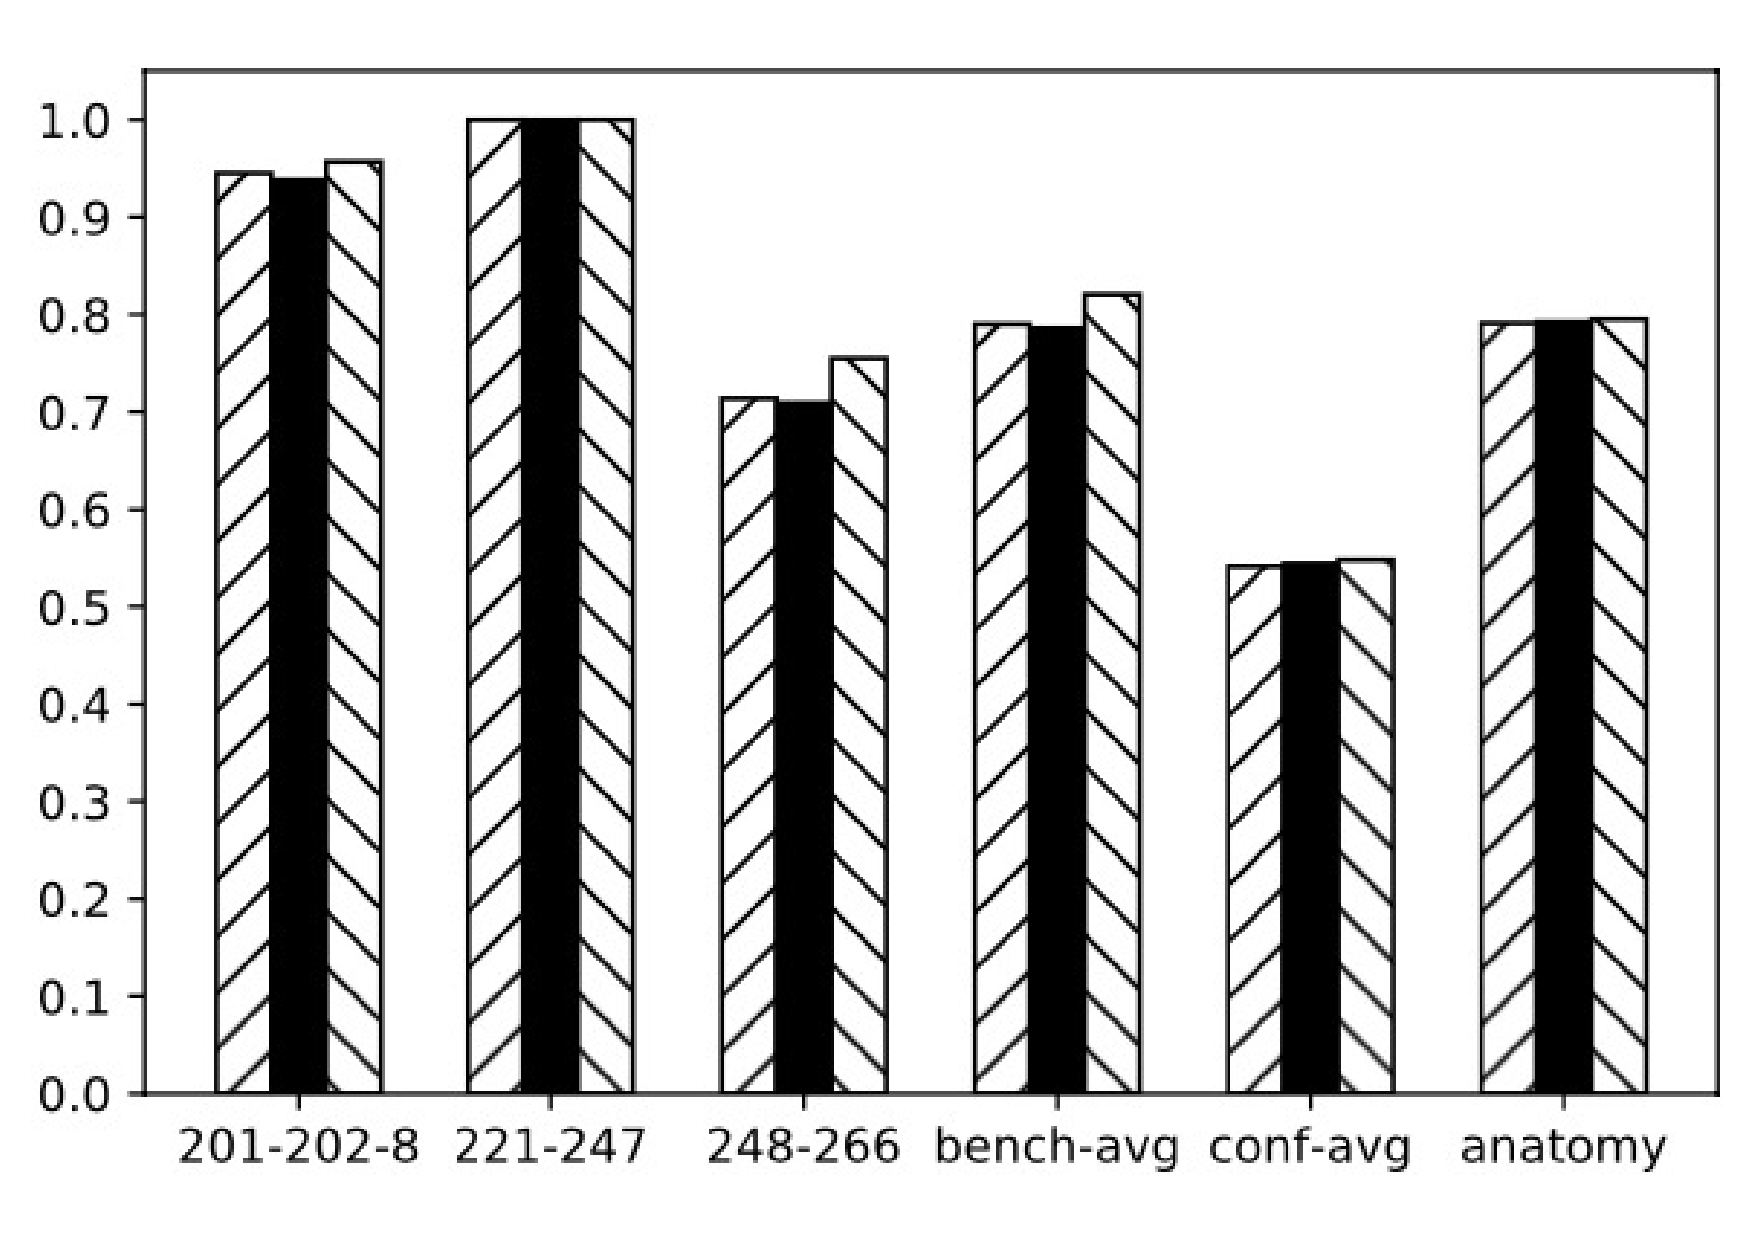
\includegraphics[width=\textwidth]{data_figs/MulRegress_Lily_R.pdf}
\caption{Recall}
\label{fig:MultiRegress_Lily_R}
\end{subfigure}
\caption{results of Lily}
\end{figure}

%\begin{figure}[htb!]\centering
%\begin{subfigure}{\textwidth}
%	\centering
%	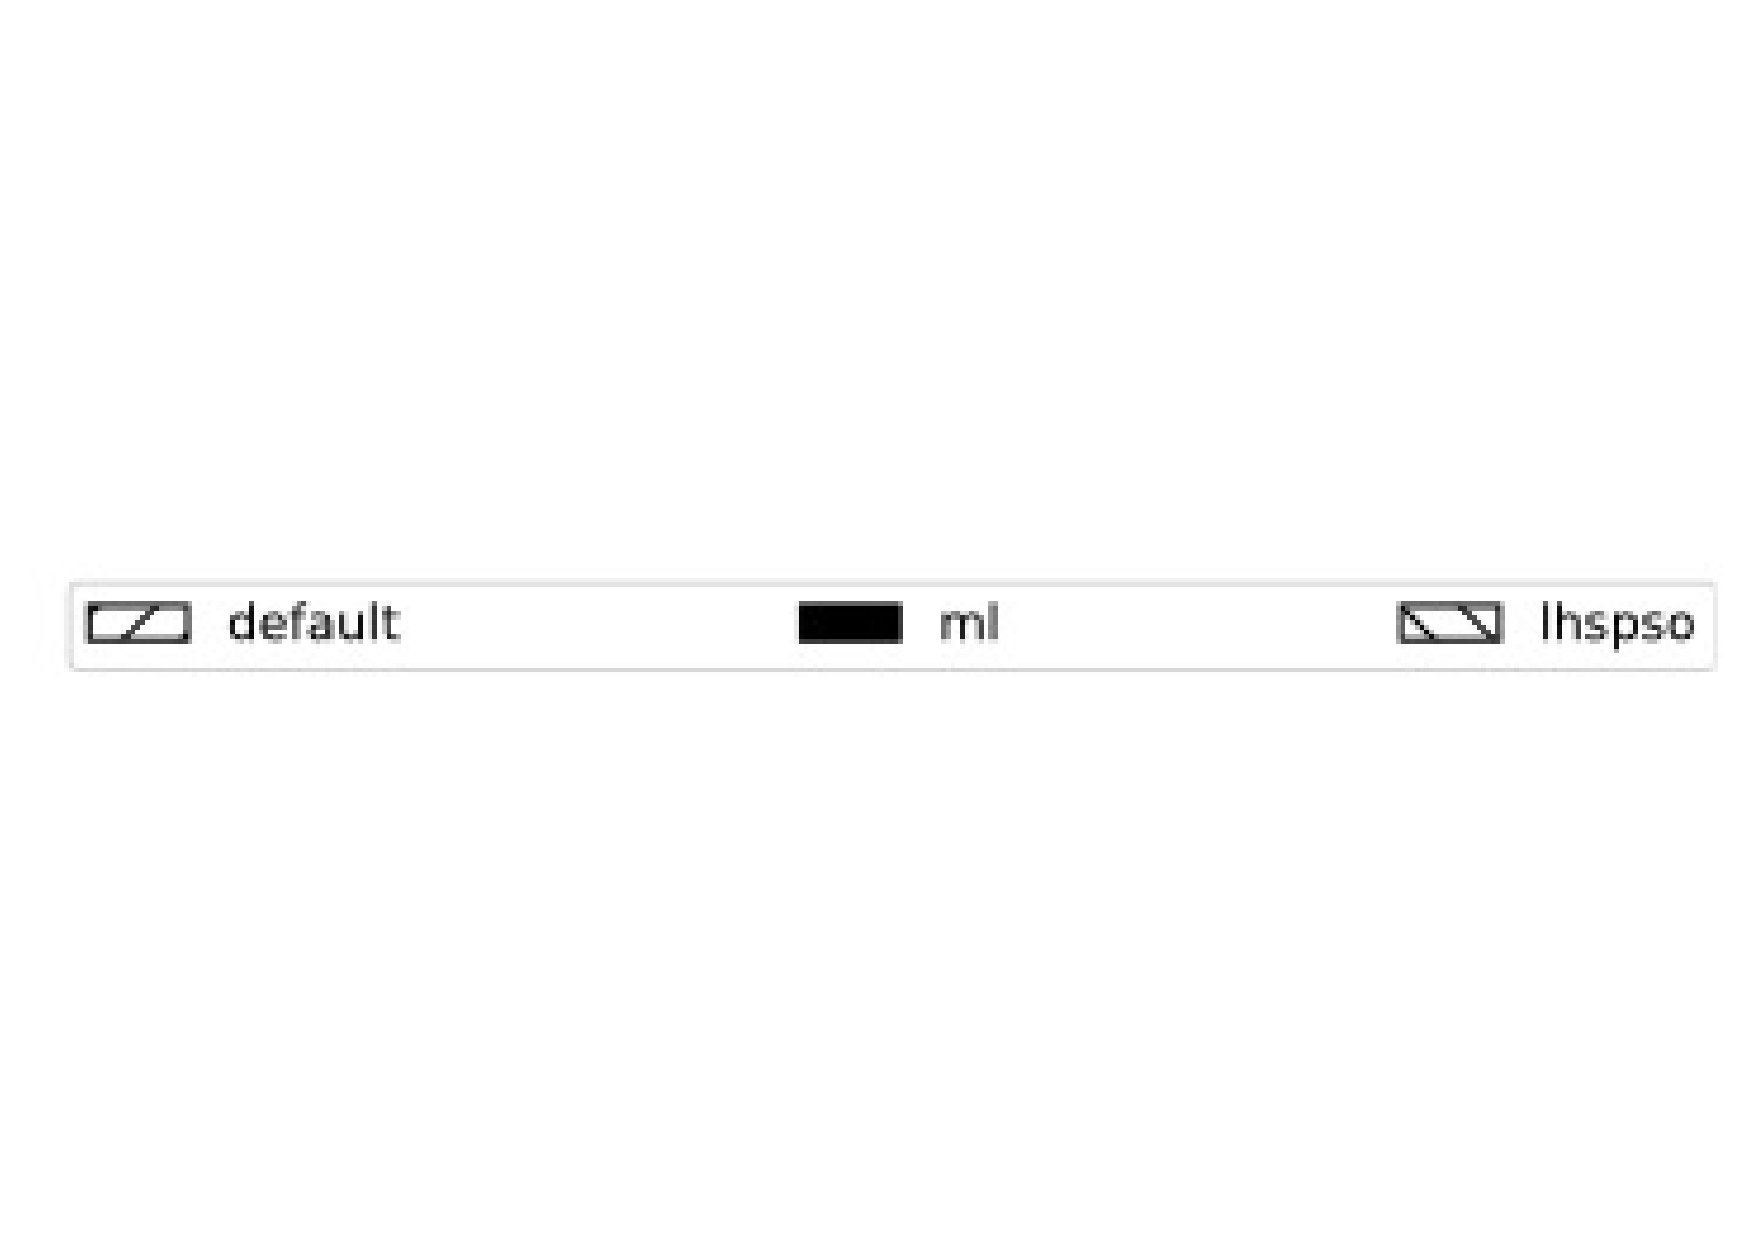
\includegraphics[width=0.45\textwidth]{figures/t_legend.pdf}
%\end{subfigure}
%\begin{minipage}{0.3\textwidth}
%	\centering
%	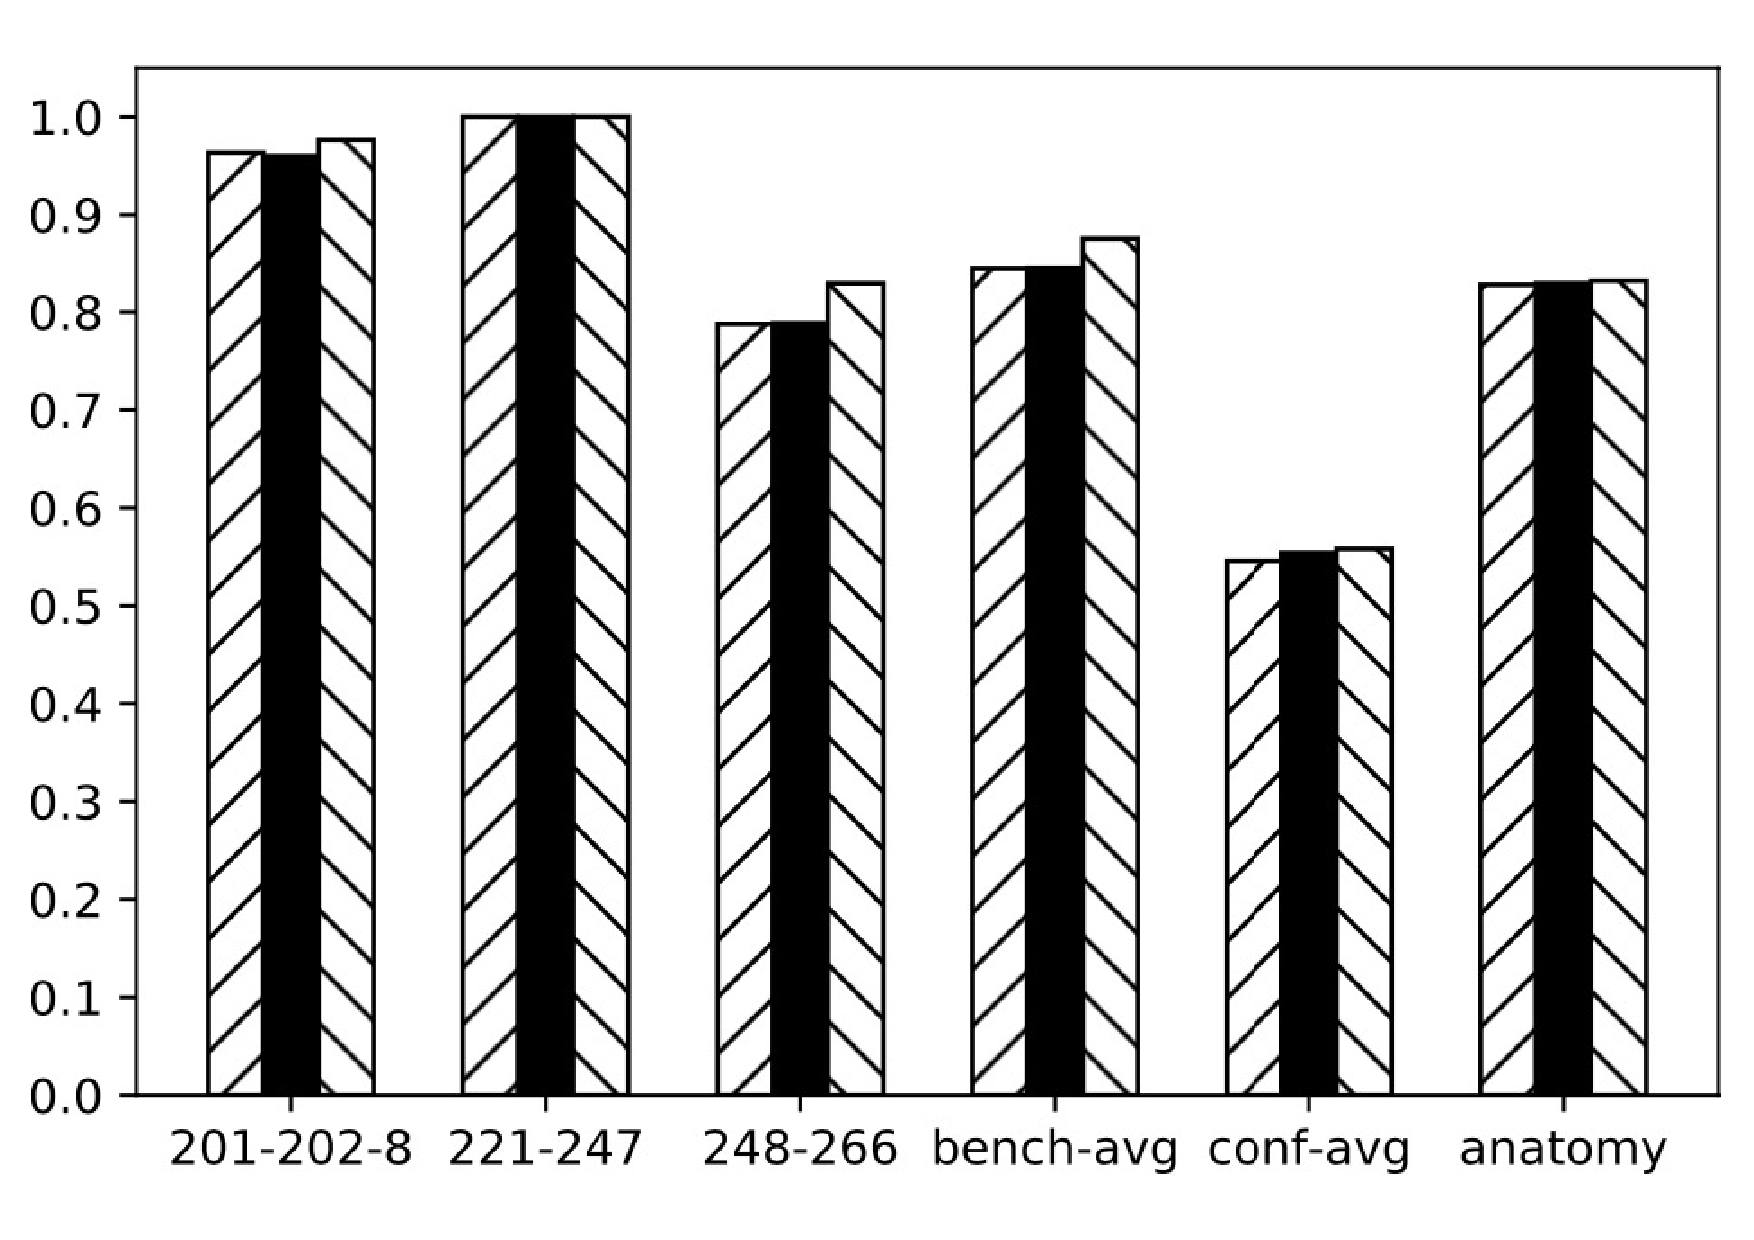
\includegraphics[width=\textwidth]{data_figs/MulRegress_Lily_F1.pdf}
%	\captionof{figure}{F1-Measure}
%	\label{fig:MulRegress_Lily_F1}
%\end{minipage}
%\begin{minipage}{0.3\textwidth}
%	\centering
%	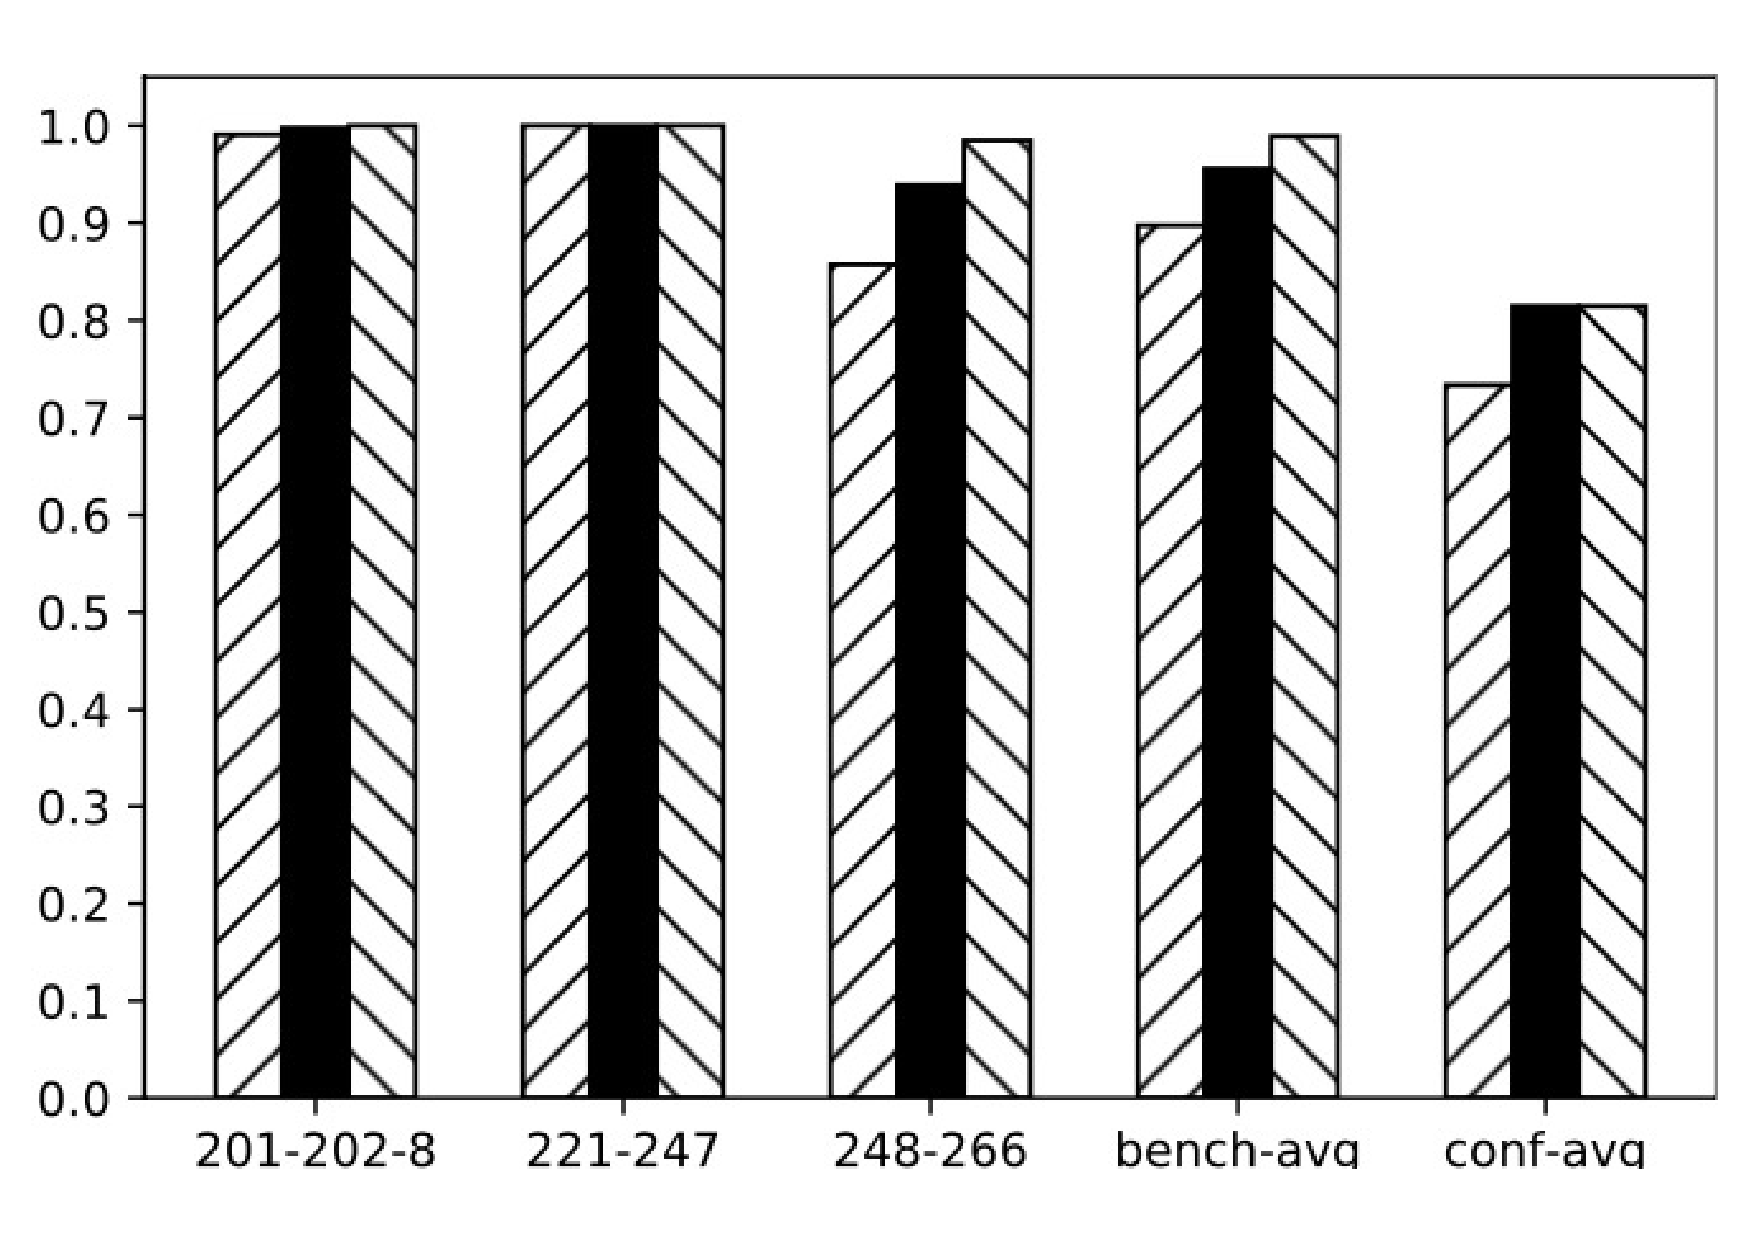
\includegraphics[width=\textwidth]{data_figs/MulRegress_RiMOM_P.pdf}
%	\captionof{figure}{Precision}
%	\label{fig:MulRegress_Lily_P}
%\end{minipage}
%\begin{minipage}{0.3\textwidth}
%	\centering
%	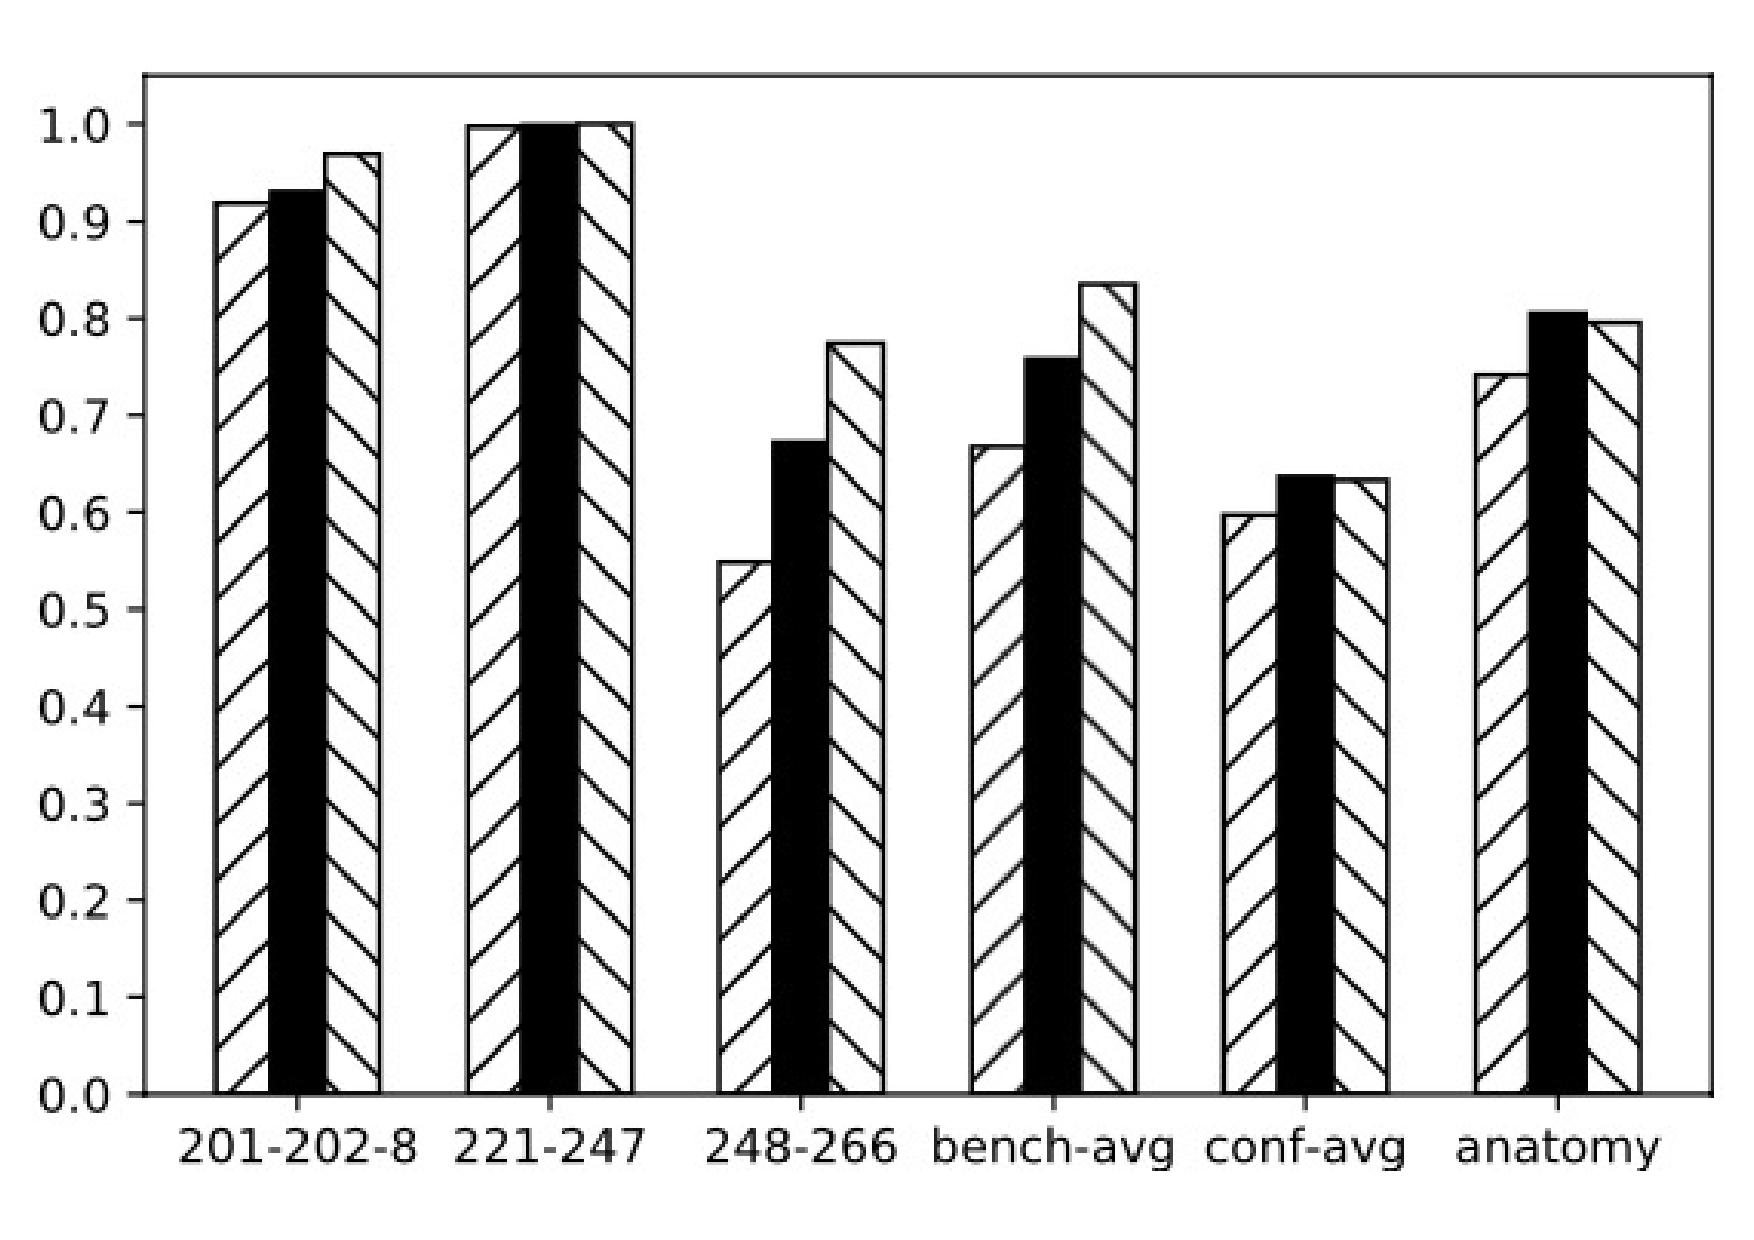
\includegraphics[width=\textwidth]{data_figs/MulRegress_Falcon_AO_R.pdf}
%	\captionof{figure}{Recall}
%	\label{fig:MulRegress_Lily_R}
%\end{minipage}
%\end{figure}

The \ref{fig:MultiRegress_LogMap_F1} shows the experimental results of the F1 value of the LogMap system.
It can be seen that on the benchmark221-247 and reference datasets, LogMap has significantly improved the matching accuracy after the ml tuning method compared to the default parameters: 3.9\% and 5.0\%, respectively.
This shows that LogMap is relatively sensitive to some matcher parameters on the real ontology data set and some parameters in the structure matcher, and changes in these parameters can easily affect the matching results.
The improvement on the anatomy dataset is not obvious, and the reason may be the same as Lily's performance on the benchmark: LogMap itself has the world's leading accuracy over the years of anatomy. The design of its built-in matching algorithm itself is already very good and it is difficult to pass Adjusting parameters to further improve the accuracy can be seen from the fact that lhspso is basically the same as the default tuning method. But in general, the experimental results of LogMap are in line with expectations, and the ml tuning method is effective on LogMap.
As for the P and R values, the improvement of the P value on the benchmark data set exceeds that of the R value, but it is the opposite on the reference data set. This shows that the overall F1 value of the LogMap system is improved on different data sets. Its dominance is also different.

\begin{figure}[htb!]\centering
\begin{subfigure}{\textwidth}
	\centering
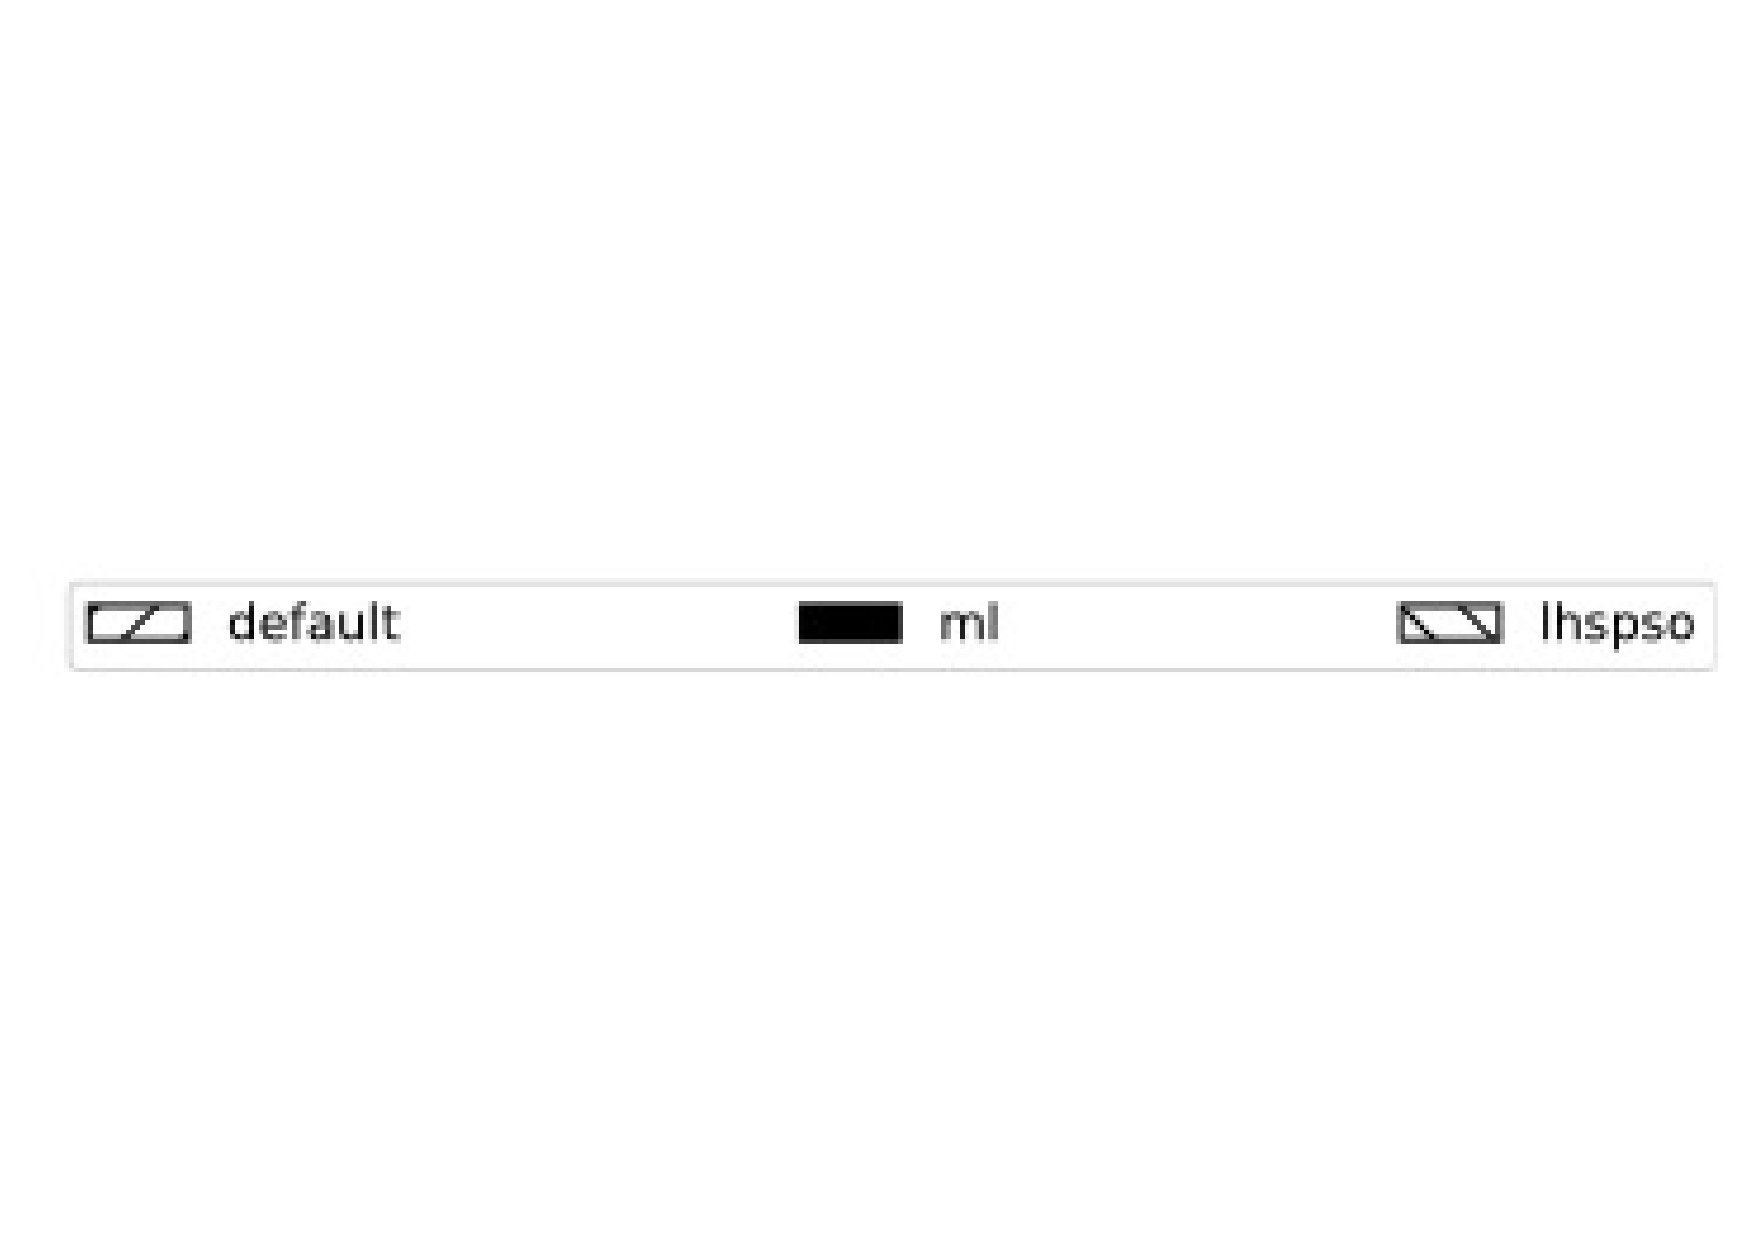
\includegraphics[width=0.45\textwidth]{figures/t_legend.pdf}
\end{subfigure}
\begin{subfigure}{0.3\textwidth}
	\centering
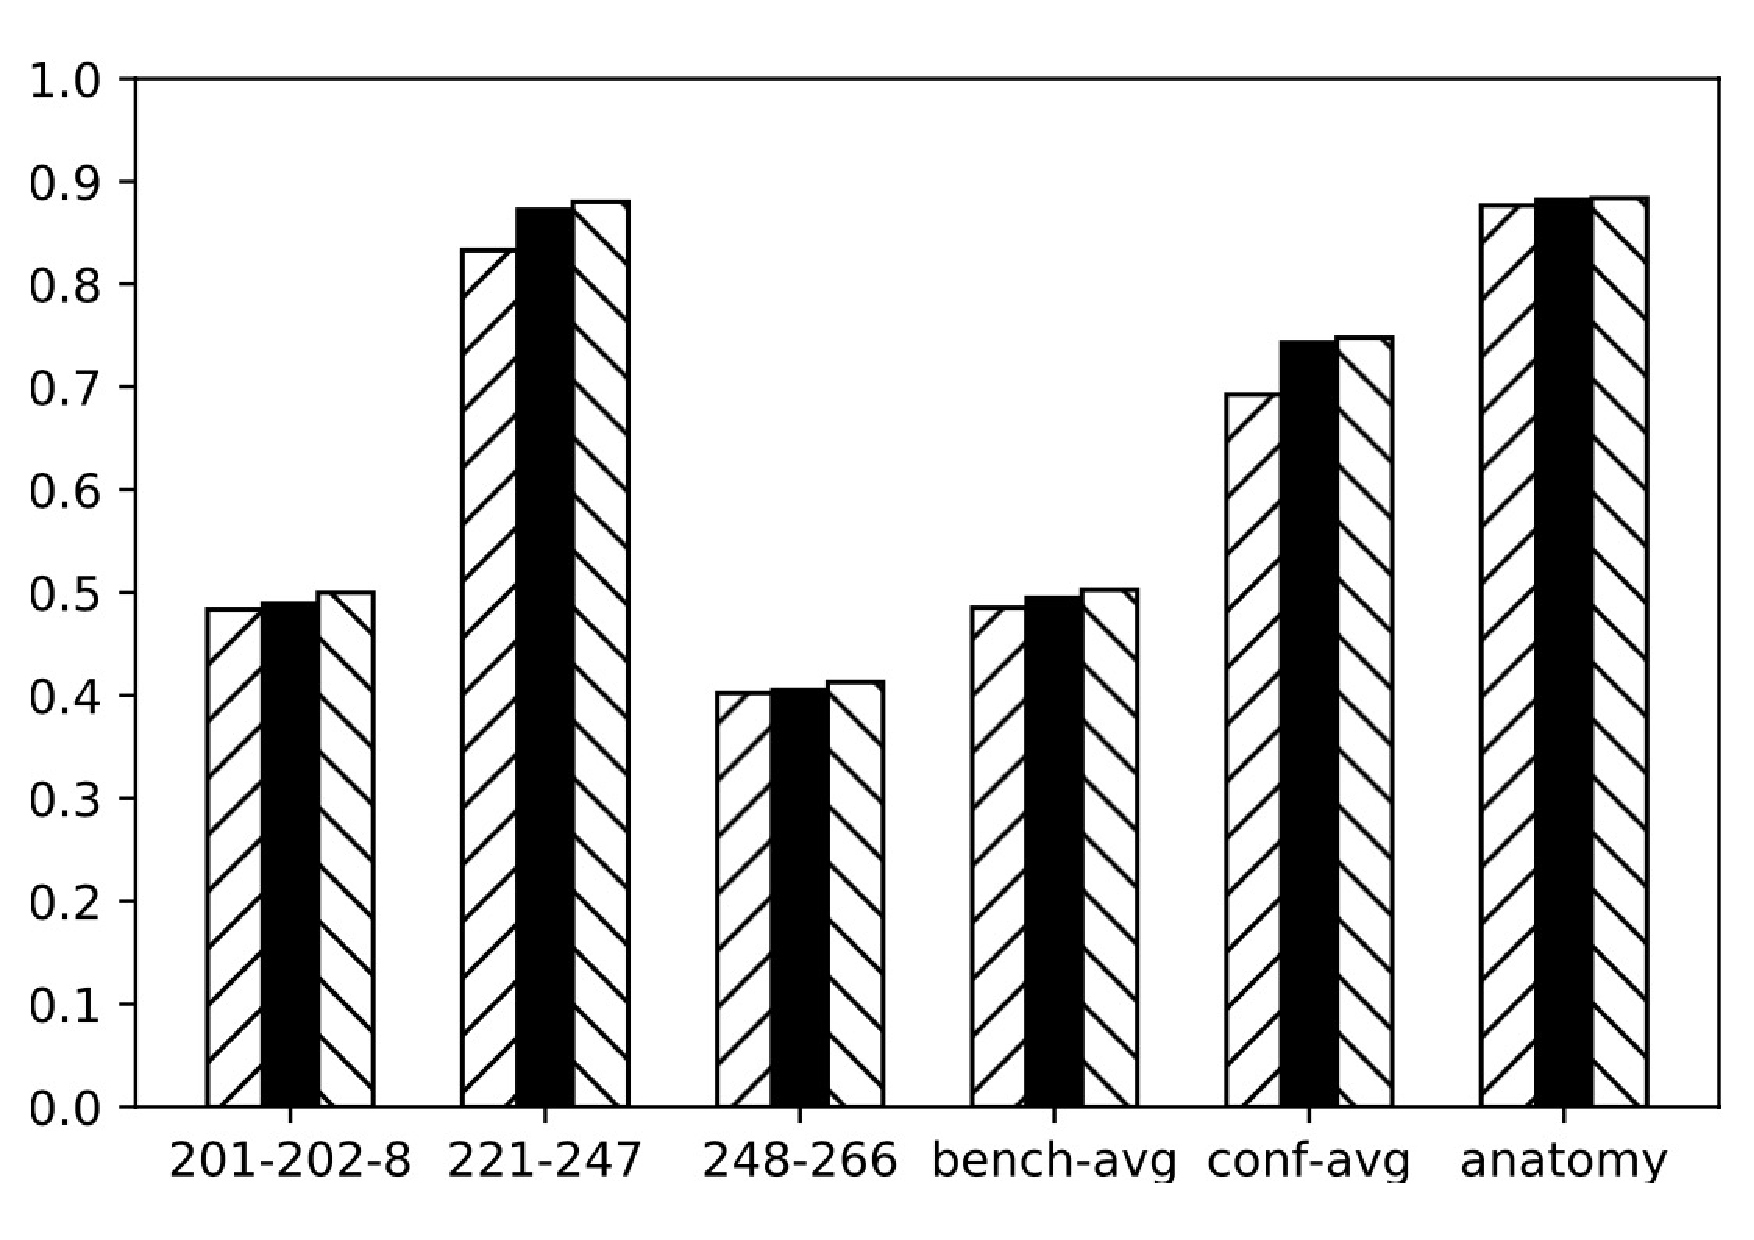
\includegraphics[width=\textwidth]{data_figs/MulRegress_LogMap_F1.pdf}
\caption{F1-Measure}
\label{fig:MultiRegress_LogMap_F1}
\end{subfigure}
%\vskip 1em
\begin{subfigure}{0.3\textwidth}
	\centering
\includegraphics[width=\textwidth]{data_figs/MulRegress_LogMap_P.pdf}
\caption{Precision}
\label{fig:MultiRegress_LogMap_P}
\end{subfigure}
\begin{subfigure}{0.3\textwidth}
	\centering
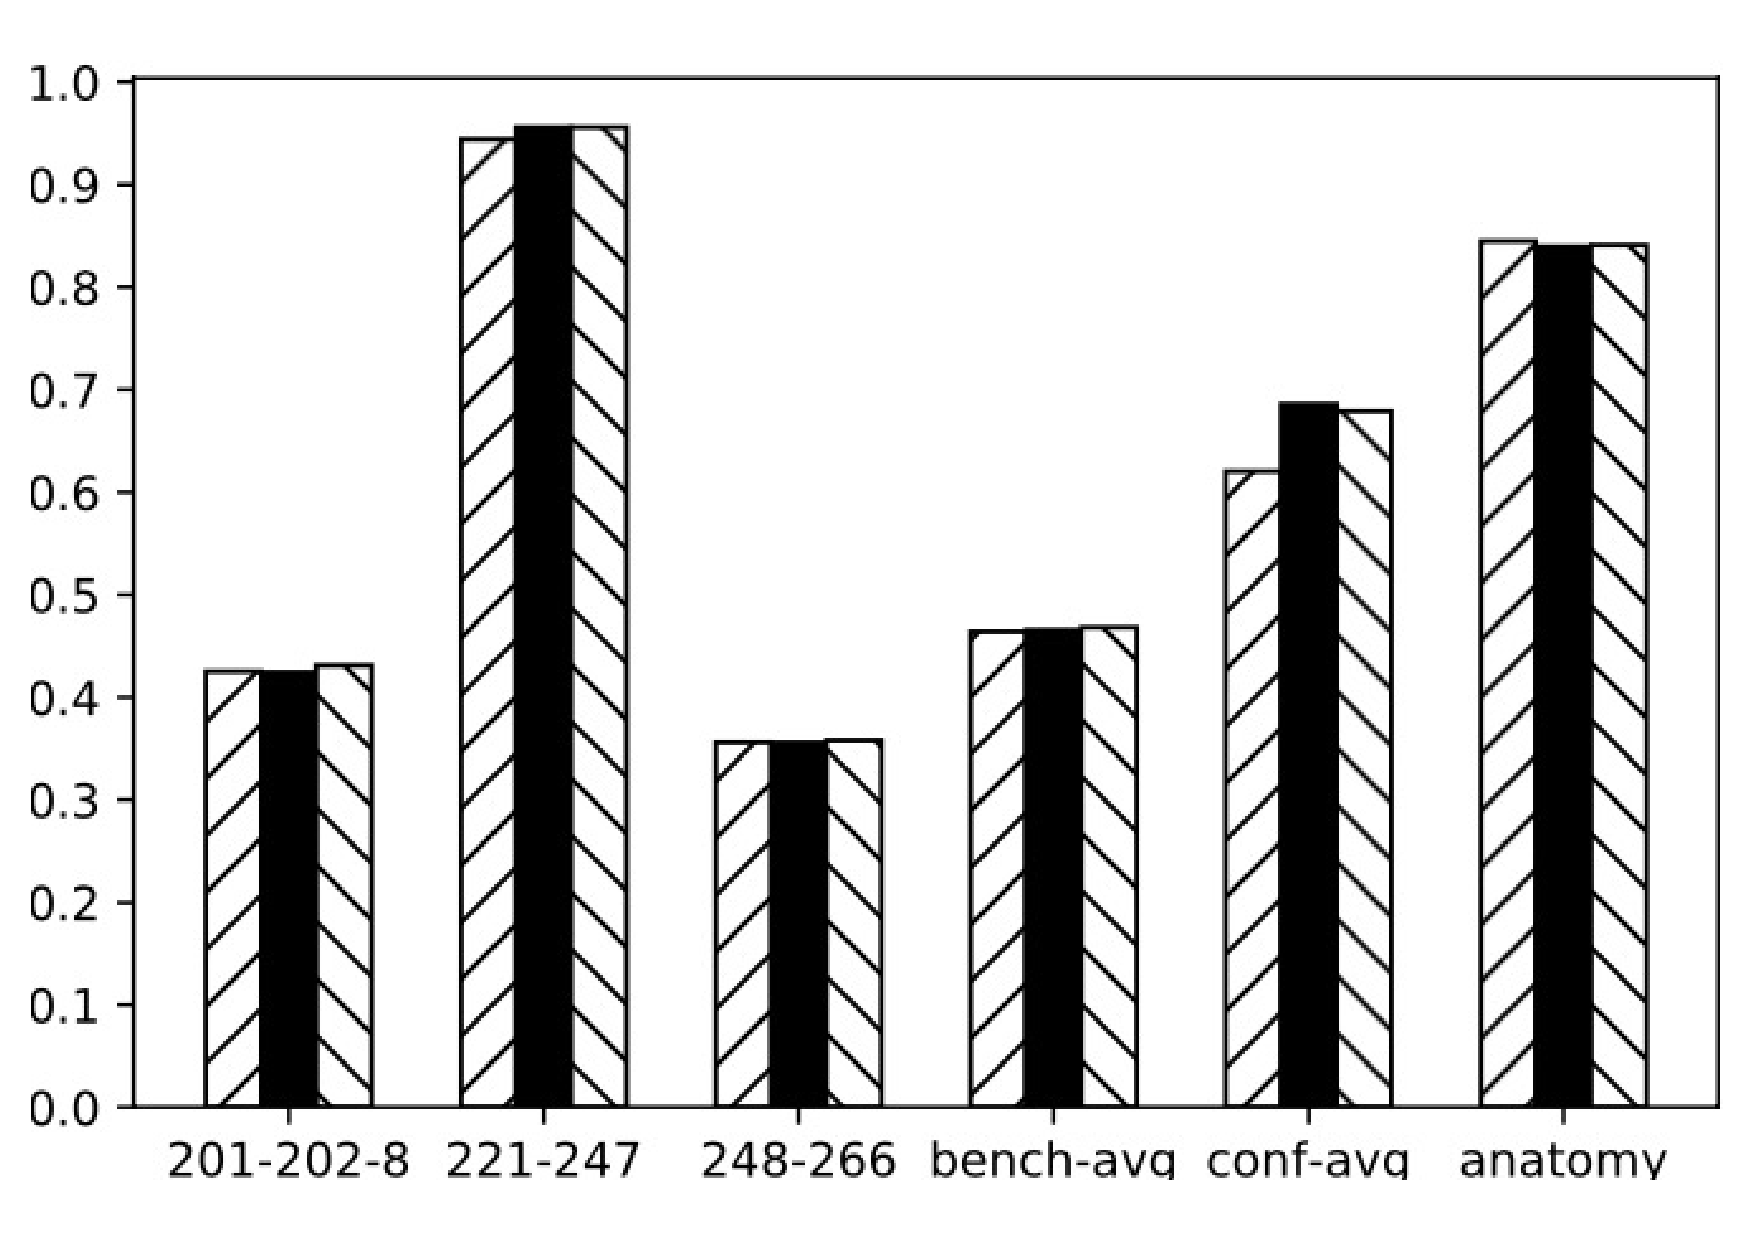
\includegraphics[width=\textwidth]{data_figs/MulRegress_LogMap_R.pdf}
\caption{Recall}
\label{fig:MultiRegress_LogMap_R}
\end{subfigure}
\caption{results of Lily}
\end{figure}

The experimental results of the F1 value of the GMap system are shown in Figure 3.14.
Similar to the RiMOM system, after GMap is tuned by ml, its matching accuracy has been significantly improved compared to the default parameters: the results on benchmark-avg and conference have approached their upper limits, increasing by 10.2\% and 3.9\%, respectively.
It is more interesting that the upper limit has been exceeded on 201-202-8, which may be due to the randomness in the GMap system.
The improvement of GMap on 221-247 is not very obvious, it may be caused by the few or less sensitive parameters in its structural matching part.
In general, the ml tuning method has achieved very good performance on the GMap system. It improves the matching accuracy obtained by the default parameters to a nearly ideal level, effectively improving the quality of the matching results and the ease of use of the GMap system.
Then, as can be seen from 3.15 and 3.16, GMap has improved the P value and R value of each data set, which shows that the great improvement of its overall F1 comes from the improvement of the two indicators.

Figure 3.17 shows the experimental results of the F1 value of the XMap system.
Overall, the ml tuning method is still effective. Although the benchmark dataset has only increased by 1.8\%, the conference dataset has increased by almost the upper limit, increasing by 4.74\%.
The benchmark improvement is not large because the improvement is small on 201-202-8. This group of tasks focuses on the text of the ontology, which indicates that the parameters of the text matcher part in XMap are not sensitive, so it is difficult to improve by adjusting the parameters.
From the graph of its P value and R value, the upper limit of the P value on 201-202-8 and 248-266 actually decreased, which shows that lhspso sacrificed a certain P value in the particle swarm search, mainly biased towards The R value is searched for the optimal solution of parameters.
Combining the two pictures of P and R at the same time, we can find that the improvement of the overall accuracy of the F1 value of the ml tuning method on the XMap system is mainly due to the improvement of the R value. This can also reflect that the internal design of the XMap system is more biased towards recall The rate, that is, hoping to find more matching pairs, can be reflected in the tuning experiment.

The last system is OLA, and its F1 value experimental results are shown in Figure 3.20.
Although the improvement of the OLA system after the ml tuning method is not obvious, it is still improved by 0.3\% and 2.46\% on the benchmark and conference respectively. Therefore, the ml tuning method is still effective on the OLA system.
The reason for the small improvement may be that the matching performance of the OLA system itself is too poor, and the built-in matching algorithm is too simple. These determine that the upper limit of tuning is not high, so it is difficult to improve the matching accuracy through parameter tuning.
Then, from the situation of the P and R values reflected in Figure 3.21 and Figure 3.22, the improvement is not obvious, for the same reasons as above.

The final Table 3.4 summarizes the results of parameter tuning of different systems on different data sets. Among them, $Ratio@P$, $Ratio@R$, $Ratio@F1$ represent the ratio of the result of the tuning to the accuracy of the ideal situation.


\subsubsection{Generality}

The generality analysis of the tuning method is mainly to analyze whether the matching effect (that is, the F1 value) of each ontology matching system on different matching tasks is improved after the tuning method is applied.

The previous analysis is based on the F1 value of the matching result. In the experiments of this paper, the F1 value is also a criterion for measuring the optimal parameters.
According to the definition, the F1 value is actually a summary of the two original experimental data indicators of accuracy (Precision value, hereinafter referred to as P value) and recall (Recall value, hereinafter referred to as R value), which can reflect to a certain extent Pros and cons of matching results.
In order not to lose the generality, the data set is used as the division, and the analysis of the two original experimental data indicators is given at the same time as the analysis of the F1 value, in an attempt to explain in which ways the method of this paper improves the matching effect.

\begin{figure}[htb!]\centering
\begin{subfigure}{\textwidth}
	\centering
\includegraphics[width=0.45\textwidth]{figures/legend.pdf}
\end{subfigure}
\begin{subfigure}{0.5\textwidth}
	\centering
\includegraphics[width=\textwidth]{data_figs/benchmark_101_F1-Measure.pdf}
\caption{F1-Measure}
\label{fig:benchmark_101_F1-Measure}
\end{subfigure}
\vskip 0.5em
\begin{subfigure}{0.49\textwidth}
	\centering
\includegraphics[width=\textwidth]{data_figs/benchmark_101_Precision.pdf}
\caption{Precision}
\label{fig:benchmark_101_Precision}
\end{subfigure}
\begin{subfigure}{0.49\textwidth}
	\centering
\includegraphics[width=\textwidth]{data_figs/benchmark_101_Recall.pdf}
\caption{Recall}
\label{fig:benchmark_101_Recall}
\end{subfigure}
\caption{The results of all systems on benchmark 101}
\end{figure}

From Figure 5.12b, it can be seen that on the 101 task of the benchmark dataset, the P value of each system matching result is similar to the F1 value, that is, the P value of most systems is not affected by the tuning method and is maintained.
At a high level; the P values of the LogMap system and the XMap system have improved to a certain extent (both are about 6.1\%). It can be seen that for these two systems, the increase in P value is a factor that drives the increase in F1 value.
It can be seen from Figure 5.12c that the R value of all systems is maintained at the highest level. The only exception is LogMap. It can be seen that each tuning method can improve its R value.
In general, the improvement of the tuning effect of the LogMap system comes from the improvement of the P and R values, while the improvement of the XMap system effect only comes from the improvement of the P value. The P and R values of other systems remain unchanged, so the tuning effect is not Variety.

\begin{figure}[htb!]\centering
\begin{subfigure}{\textwidth}
	\centering
\includegraphics[width=0.45\textwidth]{figures/legend.pdf}
\end{subfigure}
\begin{subfigure}{0.5\textwidth}
	\centering
\includegraphics[width=\textwidth]{data_figs/benchmark_201-202_F1-Measure.pdf}
\caption{F1-Measure}
\label{fig:benchmark_201-202_F1-Measure}
\end{subfigure}
\vskip 1em
\begin{subfigure}{0.49\textwidth}
	\centering
\includegraphics[width=\textwidth]{data_figs/benchmark_201-202_Precision.pdf}
\caption{Precision}
\label{fig:benchmark_201-202_Precision}
\end{subfigure}
\begin{subfigure}{0.49\textwidth}
	\centering
\includegraphics[width=\textwidth]{data_figs/benchmark_201-202_Recall.pdf}
\caption{Recall}
\label{fig:benchmark_201-202_Recall}
\end{subfigure}
\caption{The results of all systems on benchmark 201-202}
\end{figure}


In the benchmark data set, the ontology corresponding to the set of 201-202 matching tasks is obtained by replacing the entity name or comment in the original ontology with a random string. The large amount of text information in the obtained ontology will no longer have practical significance.
If the reference ratio of the text information in the ontology matching system can be reduced by adjusting the parameters, a better matching result may be obtained.
This shows the need for parameter tuning.
As can be seen from Figure 5.13a, on most ontology matching systems, the method proposed in this paper is effective, especially in the GMap and RiMOM systems.
It can also be seen that the effect of the ERT method is better than that of the History method on multiple systems. This may be because the ERT method can achieve more precise tuning of parameters.
Specifically, an ontology matching system often has multiple parameters, of which only a few may be set for the reference ratio of text information. In this group of tasks, if you focus on tuning these related parameters, you are more likely to get the desired results.

From Figure 5.13b and Figure 5.13c, it is not difficult to see that, for most systems, the improvement of the tuning effect comes from the joint improvement of the P and R values.
An interesting special case is the result of the XMap system tuning using the LHS-PSO method. It can be seen that the improvement of the final tuning effect comes from a significant increase in the R value (about 94.4\%), but many of them are reduced by the P value (about 34.6\%) Offset.
This actually reflects a problem: in the experiment, the only indicator to determine the tuning effect is the F1 value, and whether the increase in F1 value will cause other impacts (such as making the P value significantly lower) is not considered. The result of this tuning may not be exactly what the user wants.
You can consider improving the indicator, such as adding a bias measurement part to the F1 value to avoid being too biased toward the P or R value, and so on.

\begin{figure}[htb!]\centering
\begin{subfigure}{\textwidth}
	\centering
\includegraphics[width=0.45\textwidth]{figures/legend.pdf}
\end{subfigure}
\begin{subfigure}{0.5\textwidth}
	\centering
\includegraphics[width=\textwidth]{data_figs/benchmark_221-247_F1-Measure.pdf}
\caption{F1-Measure}
\label{fig:benchmark_221-247_F1-Measure}
\end{subfigure}
\vskip 1em
\begin{subfigure}{0.49\textwidth}
	\centering
\includegraphics[width=\textwidth]{data_figs/benchmark_221-247_Precision.pdf}
\caption{Precision}
\label{fig:benchmark_221-247_Precision}
\end{subfigure}
\begin{subfigure}{0.49\textwidth}
	\centering
\includegraphics[width=\textwidth]{data_figs/benchmark_221-247_Recall.pdf}
\caption{Recall}
\label{fig:benchmark_221-247_Recall}
\end{subfigure}
\caption{The results of all systems on benchmark 221-247}
\end{figure}

Different from tasks 201-202, the transformation of ontology in this group of tasks 221-2247 mainly focuses on the conceptual structure. The methods of transformation include changing or removing structural information, removing instances, removing attributes, etc.
Similarly, if the reference ratio of the structural hierarchy information in the ontology matching system can be reduced by adjusting the parameters, a better matching result may be obtained.
It can be seen from Figure 5.14a that the matching results of this group of tasks are similar to task 101. The method proposed in this paper can improve the matching results on the LogMap and XMap systems.
And compared to the 201-202 tasks, in this set of matching tasks, each system can achieve better results. This may be because each system has less dependence on the structural information in the ontology, or it can be composed of text Easily determine most matching relationships.

Similar to the situation on the 101 task, it can be seen from Figure 5.14b that the P value change trend of the matching results of each system is similar to the F1 value, that is, the P value of most systems is not affected by the tuning method and is improved. Keep at a high level; the P values of the LogMap system and the XMap system have improved to a certain extent. It can be seen that for these two systems, the rise in the P value is a factor driving the rise in the F1 value.
It can be seen from Figure 5.14c that the R values of all systems are maintained at the highest level, with the exception of LogMap and XMap. It can be seen that each tuning method can improve its R value.
In summary, the improvement of the tuning effect of the LogMap system comes from the improvement of the P and R values, while the improvement of the XMap system effect only comes from the improvement of the P value. The P and R values of other systems remain unchanged, so the tuning effect is not Variety.

\begin{figure}[htb!]\centering
\begin{subfigure}{\textwidth}
	\centering
\includegraphics[width=0.45\textwidth]{figures/legend.pdf}
\end{subfigure}
\begin{subfigure}{0.5\textwidth}
	\centering
\includegraphics[width=\textwidth]{data_figs/benchmark_248-266_F1-Measure.pdf}
\caption{F1-Measure}
\label{fig:benchmark_248-266_F1-Measure}
\end{subfigure}
\vskip 1em
\begin{subfigure}{0.49\textwidth}
	\centering
\includegraphics[width=\textwidth]{data_figs/benchmark_248-266_Precision.pdf}
\caption{Precision}
\label{fig:benchmark_248-266_Precision}
\end{subfigure}
\begin{subfigure}{0.49\textwidth}
	\centering
\includegraphics[width=\textwidth]{data_figs/benchmark_248-266_Recall.pdf}
\caption{Recall}
\label{fig:benchmark_248-266_Recall}
\end{subfigure}
\caption{The results of all systems on benchmark 248-266}
\end{figure}

248-266 The transformation of this group of tasks relative to the original ontology can be regarded as a combination of the above two sets of task transformation methods, that is, transformations that contain both text information and structural hierarchy information.
It can be seen from Figure 5.15a that the method proposed in this paper has certain effects on each ontology matching system (except that the History method will slightly reduce the effect on the two systems of Lily and LogMap, for the reason, see the results of the Lily system in section 5.2.1 Analysis).
This may be because the characteristics of the ontology in this group of tasks are relatively disturbed. Therefore, when performing the matching task, each system cannot be as sure as before to determine the matching relationship. Therefore, the internal tuning mechanism of parameter tuning is needed Make more detailed planning and adjustments.

It can be seen from Figure 5.15b and Figure 5.15c that on the 248-266 tasks, the P and R values of each system start to show some new changes with the tuning method, even though their F1 values are basically under the action of each tuning method All have risen.
The mainstream trend is still that the final effect is improved with the common increase of P and R values. The final effect of some systems is the result of the combined effect of the P value and the R value rise and fall (such as the XMap system). The effect is reduced (for example, the Lily and LogMap systems use the History method), and the reason is that the P and R values decrease together.

\begin{figure}[htb!]\centering
\begin{subfigure}{\textwidth}
	\centering
\includegraphics[width=0.45\textwidth]{figures/legend.pdf}
\end{subfigure}
\begin{subfigure}{0.5\textwidth}
	\centering
\includegraphics[width=\textwidth]{data_figs/benchmark_average_F1-Measure.pdf}
\caption{F1-Measure}
\label{fig:benchmark_average_F1-Measure}
\end{subfigure}
\vskip 1em
\begin{subfigure}{0.49\textwidth}
	\centering
\includegraphics[width=\textwidth]{data_figs/benchmark_average_Precision.pdf}
\caption{Precision}
\label{fig:benchmark_average_Precision}
\end{subfigure}
\begin{subfigure}{0.49\textwidth}
	\centering
\includegraphics[width=\textwidth]{data_figs/benchmark_average_Recall.pdf}
\caption{Recall}
\label{fig:benchmark_average_Recall}
\end{subfigure}
\caption{Average results of each system on the benchmark}
\end{figure}

Figure 5.16a shows the comparison of the average results of each ontology matching system on each task of the benchmark data set. It can be seen that after synthesizing the results of the previous groups of tasks, the method proposed in this paper has certain effects on each ontology matching system. The most obvious one is the RiMOM system. Using the ERT method can bring about 20\% improvement of F1 value.
In comparison, the improvement effect of OLA and LogMap is not very obvious, which indicates that the effect of parameter tuning will be largely restricted by the design of the ontology matching system itself.
Moreover, on all systems, the method in this paper has not yet fully achieved the effect of the LHS-PSO method, which shows that our method still has some room for improvement on the benchmark dataset.

It can be seen from Figure 5.16b and Figure 5.16c that the improvement of the effect of each system may come from the joint improvement of the P and R values, or it may be the result of the combined effect of the two.
It can also be seen that the change trend of the F1 value on each system is more similar to the change trend of the R value, which may explain that on the benchmark dataset, the main reason for the improvement in the final matching effect is the increase in the R value, or in other words, the recall Rate is the key factor to improve the matching result, and it is the difficulty of ontology matching.

\begin{figure}[htb!]\centering
\begin{subfigure}{\textwidth}
	\centering
\includegraphics[width=0.45\textwidth]{figures/legend.pdf}
\end{subfigure}
\begin{subfigure}{0.5\textwidth}
	\centering
\includegraphics[width=\textwidth]{data_figs/conference_average_F1-Measure.pdf}
\caption{F1-Measure}
\label{fig:conference_average_F1-Measure}
\end{subfigure}
\vskip 1em
\begin{subfigure}{0.49\textwidth}
	\centering
\includegraphics[width=\textwidth]{data_figs/conference_average_Precision.pdf}
\caption{Precision}
\label{fig:conference_average_Precision}
\end{subfigure}
\begin{subfigure}{0.49\textwidth}
	\centering
\includegraphics[width=\textwidth]{data_figs/conference_average_Recall.pdf}
\caption{Recall}
\label{fig:conference_average_Recall}
\end{subfigure}
\caption{Average results of each system on the conference}
\end{figure}

Figure 5.17a shows the comparison of the average results of each ontology matching system on each task of the conference dataset.
All the ontology contained in this dataset are real ontologies used to describe the organization of the conference.
It can be seen that the method proposed in this paper has certain effects on each ontology matching system.
Compared with the tuning results on the benchmark dataset, the effect of this method on the conference dataset is not so obvious, but it can also be seen that on multiple systems, our method has reached the LHS-PSO method. effect.
This illustrates the difficult nature of each system to tune on the conference dataset, and also shows that the method in this paper may be more suitable for actual ontology matching tasks, rather than the artificial ontology matching tasks related to artificially generated ontology as in the benchmark dataset.

\begin{figure}[htb!]\centering
\begin{subfigure}{\textwidth}
	\centering
\includegraphics[width=0.45\textwidth]{figures/legend.pdf}
\end{subfigure}
\begin{subfigure}{0.5\textwidth}
	\centering
\includegraphics[width=\textwidth]{data_figs/anatomy_anatomy_F1-Measure.pdf}
\caption{F1-Measure}
\label{fig:anatomy_anatomy_F1-Measure}
\end{subfigure}
\vskip 1em
\begin{subfigure}{0.49\textwidth}
	\centering
\includegraphics[width=\textwidth]{data_figs/anatomy_anatomy_Precision.pdf}
\caption{Precision}
\label{fig:anatomy_anatomy_Precision}
\end{subfigure}
\begin{subfigure}{0.49\textwidth}
	\centering
\includegraphics[width=\textwidth]{data_figs/anatomy_anatomy_Recall.pdf}
\caption{Recall}
\label{fig:anatomy_anatomy_Recall}
\end{subfigure}
\caption{Average results of each system on the anatomy}
\end{figure}

Figure \ref{fig:anatomy_anatomy_F1-Measure} shows a comparison of the results of each ontology matching system on the anatomy dataset task.
According to the information in Table 5.1, only three ontology matching systems (Falcon-AO, Lily, and LogMap) can successfully complete the test of the anatomy dataset, so the results of only three systems in the figure are compared.
Similar to the tuning results on the conference dataset, on the anatomy dataset, the method proposed in this paper has certain effects on each ontology matching system, and it is not obvious compared with the tuning results on the benchmark dataset.
But we can also see that our method has achieved the effect of the LHS-PSO method on multiple systems.
This illustrates the difficult nature of each system to tune on the anatomy dataset.
In fact, due to the large scale of the ontology in the anatomy data set, in order to be able to complete the matching task within a relatively limited time and within the constraints of hardware resources, each matching system often needs to use a relatively simpler and faster method for matching, and these The effect of the method may be less sensitive to parameter changes, which is not conducive to parameter tuning.

In the analysis of this part, it can be seen that the method in this paper has a certain effect on different ontology matching systems on multiple data sets, so it can be shown that the method proposed in this paper has certain generality.

%\subsection{Experiments of Multiple Output Regression}

\subsubsection{Effectiveness}


\subsubsection{Generality}

Figure 3.23 shows the overall F1 value performance of each matching system on the benchmark data set.
In general, after the ml tuning method, each system has a certain improvement in the matching accuracy of its default parameters and does not exceed the upper limit. This shows that on the benchmark dataset, the proposed tuning method is not only in each system The above is effective and also universal: in many different grades of matching systems, the tuning method has been improved without exception, especially in RiMOM, Falcon-AO, and GMap.

Figure 3.24 shows the overall F1 value performance of each matching system on the conference dataset.
It can be seen that in the conference data set, each system has relatively obvious default improvements without exception. Therefore, on the conference data set, our proposed tuning method also has good generality.

Figure 3.25 shows the overall F1 value performance of each matching system on the anatomy dataset.
Because there are three systems supporting the anatomy dataset, not all systems are on the map.
The anatomy task itself belongs to the category of large ontology matching, which has higher requirements on the matching algorithm itself, and the space for improvement through tuning is actually not large.
However, despite this, each system has been improved after ml tuning: from left to right, it has improved by 2.24\%, 0.57\%, and 0.14\%, respectively. This shows that the ml tuning method is still universal on anatomy.

In fact, during the experiment of tuning each system parameter, we also found some interesting phenomena and laws:

1.The fewer parameters to be tuned in the system, the more clearly the matching accuracy is improved after the ml tuning method, or the easier it is to be improved during the experiment.
The adjustable parameters of GMap and RiMOM are 3 and 5, respectively, which are relatively few. At the same time, it can be found that the accuracy improvement of these two systems after tuning is very obvious.
This phenomenon may be because the number of training samples is limited (only a few hundred). When there are fewer parameters in the system, the multi-output regression model is easier to learn the relationship between parameters and parameters. It will inevitably increase the learning cost of the model, and its prediction effect will also decrease, leading to a less significant improvement in accuracy. There are relatively many parameters to be adjusted in LogMap, Lily, and OLA, so it is difficult to improve the subsequent accuracy.

2.When a system is improved by the lhspso tuning method compared to the default, that is, if the upper limit is high, the system can easily obtain a significant accuracy improvement through the ml tuning method.
Although the Falcon-AO system has as many as 26 adjustable parameters, if from the perspective of the model, so few training samples are not conducive to model learning, but as shown in Figure 3.2, Falcon-AO The upper limit of the F1 value that can be improved is very high, so it still has a significant accuracy improvement after the ml tuning method. It can be understood that the high limit indicates that the system has great potential for improvement after tuning.
Conversely, if the upper limit itself is not high, the increase will not be too obvious after the ml tuning, because it will not exceed this upper limit.

3.The randomness of the built-in algorithm of the system will affect the prediction effect of the regression model.
Because each match has different F1 values if it is run multiple times under the same parameter configuration, this will inevitably affect the approximate optimal solution searched by the particle swarm algorithm and cause the training set to have randomness, which will affect the model prediction effect influences.

In the analysis of the above experimental results, we demonstrated the ml tuning method from the perspectives of effectiveness and versatility.
The experimental results show that the ml tuning method is not only effective on each matching system, that is, it can improve the ease of use of the ontology matching system and the tuning accuracy of each system after tuning has been improved to some extent compared to the default; and The tuning method is also very versatile. It can play a role in many different grades of ontology matching systems, and it can be a universal module in the ontology matching system.

\subsubsection{Experiment of Machine Learning-Based Policy Tuning}

For the strategy tuning method based on supervised learning, the training set of the experimental part is consistent with the test set and parameter tuning. It still uses the three classic task benchmarks, conferences, and anatoms for OAEI experiments, and the three years of OAEI 2012, 2013, and 2015. Data for training, OAEI2016 year for data testing.
The indicators of the result evaluation are still the P value, R value and F1 value.
The experimental matching system here is a newly developed Lily-TM (Tuning Mapper) with a strategy tuning function.
Lily-TM's matching algorithm for large ontology anatomy tasks is a direct reuse Lily system. Before the experiment, all the adjustable strategies in Lily's built-in large ontology matching algorithm were found in advance, and a strategy tuning module was implanted in it.
The rest of the standard benchmark and conference datasets are still tested with Lily-TM.
The specific experimental steps are to first use the data from the previous three years to build the training set. Specifically, for each set of offline matching tasks, perform a DFS depth-first search in advance to obtain the optimal strategy as the category label of the task sample. Second, use the training set to train the classification. The model and the trained model are built into the Lily-TM system; finally, for unknown matching tasks in the test set, automatic prediction of the strategy path is performed according to its different task characteristics, thereby realizing fully automatic strategy tuning.

%\subsubsection{Results and Analysis}

Similar to parameter tuning, the experimental comparison object in strategy tuning still has a set of default strategies. In this section, Avg+Threshold, Harmony+NaiveAscending, Max+Hungarian, Sigmoid+Threshold are used as the default strategies.
Take the {\it Avg+Threshold} strategy as an example, which means that after the similarity matrix is calculated, the simple similarity method is used to obtain the final similarity matrix, and then the final matching result is extracted from the final similarity matrix by the threshold method. similar.
{\it ADAPT\_SL} (Supervised Learning) in the figure below shows the matching result of the system after the automatic strategy tuning method based on supervised learning

In the course of the experiment, the necessity of strategy tuning was indeed discovered.
It is observed in the experiment that the optimal strategy is different in different matching tasks.
For example, simple tasks such as simple average fusion and threshold extraction can achieve good matching accuracy; but some tasks require a slightly more complicated harmony algorithm to perform better in the fusion process; some tasks use the matching extraction module. The threshold method has a poor effect but it works well with greedy descending extraction; there are other tasks that use simple average fusion and greedy extraction etc., which are better than harmony fusion and greedy extraction.
In short, for each type It is necessary and meaningful to automatically predict the optimal matching strategy path for different tasks.
The following are detailed experimental results on different data sets. All results use F1 value as the evaluation index.

Figure 4.6 depicts the experimental results of strategy tuning on the benchmark dataset.
In general, the ADAPT strategy after automatic strategy tuning has a higher matching accuracy than the other default fixed strategies, which shows that the strategy tuning methods based on supervised learning proposed in this chapter are very effective.
On this data set, the ADAPT\_SL strategy has an average accuracy improvement of 25.94\% compared to several other default fixed strategies.
Among the 248-266 tasks, the ADAPT\_SL strategy is almost 45\% higher than the worst performing strategy SIGMOID+THRESHOLD.
Under the 221-2247 task, the ADAPT\_SL strategy is not significantly higher than the average value of the remaining individual strategies. Large, it may be that this group of tasks is biased to the structure, and the structure matcher of Lily-TM itself is weak, so its upper limit of tuning is low, and it is difficult to exert the effect of strategy tuning.

As shown in Figure 4.7, on the conference dataset, the ADAPT strategy has improved by an average of 15\% compared to several other default fixed strategies. This shows that the automatic strategy tuning method is still effective on the real dataset, but the overall strategy The lower F1 value may be due to the weak performance of the matching algorithm for the real ontology dataset in the Lily-TM system.

Finally, the anatomy data set is shown in Figure 4.8. The ADAPT\_SL after strategy tuning is 5.54\% higher than Lily's default strategy path, which indicates that Lily's original built-in single strategy is not optimal. The strategy is used in different scenarios. After the automatic switching, there is still some room for improvement.

In summary, the detailed experimental results on various data sets prove that the method of automatic tuning based on machine learning strategies proposed in this chapter is effective and feasible.
The strategy tuning method based on supervised learning can automatically find a relatively optimal matching strategy according to the characteristics of different matching tasks and according to the rules learned previously by the model.
This method effectively improves the ease of use of the matching system and further improves The quality of the matching results.
\section{Conclusions}

In this paper, we propose a series of novel approaches to solve the ontology matching tuning problem.
For parameter tuning, a approaches for tuning ontology matching parameters based on similarity analysis and a approaches based on extreme random forest are proposed.
The former searches for historical ontology matching tasks to find and apply parameters that are most suitable for the current ontology matching task.
The latter learns the correspondence between the characteristics of the historical matching task and the optimal parameters and applies it to the current ontology matching task to optimize its tuning.
In addition, matching strategy tuning is considered as a multi-classification problem and is solved using a learning-based approach.

The experimental results show that the approaches proposed in this paper can be effective on many different ontology matching systems and different kinds of ontology matching data sets, and has high tuning efficiency, which can greatly reduce the workload of artificial ontology matching.

\vspace{2mm}

\begin{thebibliography}{99}
\footnotesize
\itemsep=-3pt plus.2pt minus.2pt
\baselineskip=13pt plus.2pt minus.2pt
\bibitem{wwy1}Studer R, Benjamins V R, Fensel D. Knowledge engineering: principles and methods. {\it Data and knowledge engineering}, 1998, 25(122):161-197.

\bibitem{wwy2}Gruber T R. A translation approach to portable ontology specifications. {\it Knowledge acquisition}, 1993, 5(2):199-220.

\bibitem{wwy3}Kitchenham B A, Pfleeger S L, Pickard L M, {\it et al.} Preliminary guidelines for empirical research in software engineering. {\it IEEE Trans. Software Engineering}, 2002, 28(8):721-734.

\bibitem{wwy4}Shum S B, Motta E, Domingue J. ScholOnto: an ontology-based digital library server for research documents and discourse. {\it International Journal on Digital Libraries}, 2000, 3(3):237-248.

\bibitem{wwy5}Roman D, Keller U, Lausen H, {\it et al.} Web service modeling ontology {\it Applied ontology}, 2005, 1(1):77-106.

\bibitem{wwy6}Berners-Lee T, Hendler J, Lassila O, {\it et al.} The semantic web. {\it Scientific american}, 2001, 284(5):28-37.

\bibitem{wwy7}Studer R, Benjamins V R, Fensel D. Knowledge engineering: principles and methods. {\it Data and knowledge engineering}, 1998, 25(122):161-197.

\bibitem{wwy8}Ding L, Finin T, Joshi A, {\it et al.} Swoogle: a search and metadata engine for the semantic web. {\it Proc. the 13th ACM Int. Information and knowledge management}, 2004. 652-659.

%\bibitem{wwy9} 9 邓志鸿, 唐世渭, et al. Ontology 研究综述 [J]. 北京大学学报: 自然科学版, 2002, 38(5):730-738.
\bibitem{wwy10} Falconer S M, Noy N F, Storey M A D. Ontology Mapping-a User Survey.In {\it Proc. the 2nd Int. Ontology Matching}, November, 2007. Volume 304, pp. 49-60.
%Falconer, S. M., Noy, N. F., & Storey, M. A. (2007, November). Ontology mapping: a user survey. In Proceedings of the 2nd International Conference on Ontology Matching-Volume 304 (pp. 49-60). CEUR-WS. org.
\bibitem{wwy11} Van Harmelen F. Ontology mapping: a way out of the medical tower of Babel? In {\it Proceedings of the 10th Conference on Artificial Intelligence in Medicine}, pp.3-6.
%Van Harmelen, F. (2005, July). Ontology mapping: A way out of the medical tower of babel?. In Conference on Artificial Intelligence in Medicine in Europe (pp. 3-6). Springer, Berlin, Heidelberg.
\bibitem{wwy12} Hovy, E. Combining and standardizing large-scale, practical ontologies for machine translation and other uses. In {\it Proceedings of the 1st International Conference on Language Resources and Evaluation}, pp. 535-542.
%Hovy, E. (1998, May). Combining and standardizing large-scale, practical ontologies for machine translation and other uses. In Proceedings of the 1st International Conference on Language Resources and Evaluation (LREC) (pp. 535-542).
\bibitem{wwy13} Lopez, V., Motta, E., \& Uren, V. Poweraqua: Fishing the semantic web. In {\it European Semantic Web Conference}, pp.393-410.
%Lopez, V., Motta, E., & Uren, V. (2006, June). Poweraqua: Fishing the semantic web. In European Semantic Web Conference (pp. 393-410). Springer, Berlin, Heidelberg.
\bibitem{wwy14} Kalfoglou Y, Schorlemmer M. Ontology mapping: the state of the art. {\it The knowledge engineering review}, 2003, 18(01):1-31.
\bibitem{wwy15} Rahm E, Bernstein P A. A survey of approaches to automatic schema matching. {\it the VLDB Journal}, 2001, 10(4):334-350.


\bibitem{wwy16} Shvaiko P, Euzenat J. A survey of schema-based matching approaches. In {\it Journal on Data Semantics IV}, 2005. pp.146-171.
\bibitem{wwy17} Wache H, Voegele T, Visser U, {\it et al.} Ontology-based integration of information-a survey of existing approaches. In: {\it IJCAI-01 workshop: ontologies and information sharing}, 2001. pp.108-117.
\bibitem{wwy18} Shvaiko P, Euzenat J. Ontology matching: state of the art and future challenges. {\it IEEE Transactions on knowledge and data engineering}, 2013, 25(1):158-176.
\bibitem{wwy19} Noy N F. Semantic integration: a survey of ontology-based approaches. {\it ACM Sigmod Record}, 2004, 33(4):65-70.
\bibitem{wwy20} Uschold M, Gruninger M. Ontologies and semantics for seamless connectivity. {\it ACM SIGMod Record}, 2004, 33(4): 58-64.
\bibitem{wwy21} Euzenat J, Le Bach T, Barrasa J, et al. State of the art on ontology alignment. {\it Knowledge Web Deliverable D}, 2004, 2:2-3.
\bibitem{wwy22} Predoiu L, Feier C, Scharffe F, et al. State-of-the-art survey on Ontology Merging and Aligning. {\it SEKT: Semantically Enabled Knowledge Technologies, University of Innsbruck}, 2004.
\bibitem{wwy23} Stoilos G, Stamou G, Kollias S. A string metric for ontology alignment. In {\it International Semantic Web Conference}, 2005. 624-637.
\bibitem{wwy24} Van Hage W R, Katrenko S, Schreiber G. A method to combine linguistic ontology-mapping techniques. In {\it International Semantic Web Conference}, 2005. 732-744.
\bibitem{wwy25} Hu W, Jian N, Qu Y, et al. Gmo: A graph matching for ontologies. In {\it Proceedings of K-CAP Workshop on Integrating Ontologies}, 2005. 41-48.
\bibitem{wwy26} Noy, N. F., Musen, M. A. The PROMPT suite: interactive tools for ontology merging and mapping. {\it International journal of human-computer studies}, 59(6), 983-1024.
\bibitem{wwy27} Doan A, Madhavan J, Domingos P, et al. Learning to map between ontologies on the semantic web. In {\it Proceedings of the 11th international conference on World Wide Web}, 2002. 662-673.
\bibitem{wwy28} Isaac A, Van Der Meij L, Schlobach S, et al. An empirical study of instance-based ontology matching. In {\it The Semantic Web} The Semantic Web. 2007. 253-266.
\bibitem{wwy29} Kotis K, Vouros G A. The HCONE approach to ontology merging. In {\it The Semantic Web: Research and Applications}, 2004. 137-151.
\bibitem{wwy30} Giunchiglia F, Yatskevich M, Shvaiko P. Semantic matching: Algorithms and implementation. In {\it Journal on Data Semantics IX},  2007. 1-38.
\bibitem{wwy31} Tang, J., Li, J., Liang, B., Huang, X., Li, Y., \& Wang, K. Using Bayesian decision for ontology mapping. {\it Web Semantics: Science, Services and Agents on the World Wide Web}, 4(4), 243-262.
%\bibitem{wwy32} 32 唐杰, 梁邦勇, 李涓子, et al. 语义 Web 中的本体自动映射 [J]. 计算机学报, 2007, 29(11):1956-1976.
\bibitem{wwy33} Ehrig M, Sure Y. Foam-framework for ontology alignment and mapping results of the ontology alignment evaluation initiative. In {\it Integrating Ontologies Workshop Proceedings}, 2005. 72.
\bibitem{wwy34} Hu W, Qu Y. Falcon-AO: A practical ontology matching system. {\it Web Semantics: Science, Services and Agents on the World Wide Web}, 2008, 6(3):237-239.
\bibitem{wwy35}Shvaiko P., Euzenat J. Ten Challenges for Ontology Matching. In {\it On the Move to Meaningful Internet Systems: OTM 2008.}, 2008, pp.237-239

\bibitem{wwy36}Mochol M., Jentzsch A. Towards a rule-based matcher selection. {\it Knowledge Engineering: Practice and Patterns.}, 2008, 109-119.

\bibitem{wwy37}Eckert K., Meilicke C., Stuckenschmidt H. Improving ontology matching using meta-level learning. {\it The Semantic Web: Research and Applications.}, 2009, pp.158-172

\bibitem{wwy38}Lee Y, Sayyadian M, Doan A, et al. eTuner: tuning schema matching software using synthetic scenarios. {\it The International Journal on Very Large Data Bases}, 2007, 16(1):97-122.

\bibitem{wwy39}Thummala V, Babu S. iTuned: a tool for configuring and visualizing database parameters. In {\it Proceedings of the 2010 ACM SIGMOD International Conference on Management of data}, June,2010, pp.1231-1234.

\bibitem{wwy40}Duan S, Thummala V, Babu S. Tuning database configuration parameters with iTuned. {\it Proceedings of the VLDB Endowment}, 2009, 2(1):1246-1257.

\bibitem{wwy41}Xi B, Liu Z, Raghavachari M, et al. A smart hill-climbing algorithm for application server configuration. In {\it Proceedings of the 13th international conference on World Wide Web.}, 2004, pp.287-296

% \bibitem{wwy42}Zhou Y. Extensions of an Empirical Automated Tuning Framework.2013. https://drum.lib.umd.edu/bitstream/handle/1903/14298/Zhou_umd_0117N_14258.pdf

\bibitem{wwy43}Mao M, Peng Y, Spring M. A Harmony based Adaptive Ontology Mapping Approach. In {\it SWWS.}, 2008, pp.336-342.

\bibitem{wwy44}Niu X, Wang H, Wu G, et al. Evaluating the stability and credibility of ontology matching methods. In{\it The Semantic Web: Research and Applications.}, 2011, pp.275-289

\bibitem{wwy45}Meilicke C, Stuckenschmidt H. Analyzing Mapping Extraction Approaches. In {\it Proceedings of the 2nd International Conference on Ontology Matching - Volume 304.}, 2007.

\bibitem{wwy46}Bock J, Hettenhausen J. Discrete particle swarm optimisation for ontology alignment. {\it Information Sciences, 2012, 192:152-173}, 2012, 192:152-173.

\bibitem{wwy47}Abd-El-Wahed W, Mousa A, El-Shorbagy M. Integrating particle swarm optimization with genetic algorithms for solving nonlinear optimization problems. {\it Journal of Computational and Applied Mathematics}, 2011, 235(5):1446-1453.

\bibitem{wwy48}Yang P, Wang P, Ji L, et al. Ontology Matching Tuning Based on Particle Swarm Optimization: Preliminary Results. In {\it Chinese Semantic Web and Web Science Conference.}, 2014, pp.146-155.

\bibitem{wwy49}Ritze D, Paulheim H. Towards an automatic parameterization of ontology matching tools based on example mappings. {\it CEUR Workshop Proceedings.}, 2011. 814:37.

\bibitem{wwy50}CruzIF,FabianiA,CaimiF,etal. Automatic configuration selection using ontology matching task profiling. In {\it The Semantic Web: Research and Applications.}, 2012, pp.179-194.

\bibitem{wwy51}Maedche A, Staab S. Measuring similarity between ontologies. In {\it International Conference on Knowledge Engineering and Knowledge Management.}, 2002, pp.251-263.

\bibitem{wwy52}Kuhn H W. The Hungarian method for the assignment problem. {\it Naval research logistics quarterly}, 1955, 2(1-2):83-97.

\bibitem{wwy53}Levenshtein V I. Binary codes capable of correcting deletions, insertions, and reversals. {\it Soviet physics doklady.}, 1966. 10:707-710.

\bibitem{wwy54}Geurts P, Ernst D, Wehenkel L. Extremely randomized trees. {\it Machine learning},  2006, 63(1):3-42.

\bibitem{wwy58}Euzenat J., Ehrig M., Castro R. Towards a Methodology for Evaluating Alignment and Matching Algorithms. {\it Technical Report, Ontology Alignment Evaluation Initiative.}, 2005.

\bibitem{wwy59}C. J. van RIJSBERGEN B.Sc. Information Retrieval. USA: Butterworth-Heinemann, 1979.

\end{thebibliography}



\label{last-page}
%\end{multicols}
\label{last-page}
\end{document}

